\documentclass[12pt,a4paper,titlepage]{article}
\usepackage[utf8]{inputenc}
\usepackage[russian,english]{babel}
\usepackage[usenames]{color} %!!
\usepackage{colortbl} %!
\usepackage{amsmath}
\numberwithin{equation}{section}
\usepackage{bm}
\usepackage{amsfonts}
\usepackage{amssymb}
\usepackage{mathrsfs}
\usepackage{indentfirst}
\usepackage{slashed}
\usepackage[hidelinks]{hyperref}
\usepackage[ddmmyyyy]{datetime}
\usepackage{epigraph}
\usepackage{graphicx}
\usepackage{cancel}
\graphicspath{{fig/}}
\usepackage[subnum]{cases}
\usepackage{accents}
\usepackage[left=3cm,right=2cm,top=2cm,bottom=2cm]{geometry}
\DeclareMathOperator{\Div}{div}
\DeclareMathOperator{\Rot}{rot}
\DeclareMathOperator{\Grad}{grad}
\DeclareMathOperator{\Arsh}{Arsh}
\DeclareMathOperator{\const}{const}
\DeclareMathOperator{\inv}{inv}
\newcommand{\parder}[2]{\dfrac{\partial {#1}}{\partial {#2}}}
\newcommand{\vecmult}[2]{\left[ \vec{{#1}} \times \vec{{#2}}   \right]}
\newcommand{\abs}[1]{\left| #1  \right|}
\newcommand{\half}{\frac{1}{2}}
\newcommand{\kv}{\vec{k}}
\renewcommand{\vec}[1]{\mathbf{#1}}
\renewcommand{\Re}{\operatorname{Re}}
\renewcommand{\Im}{\operatorname{Im}}
\newcommand{\Tr}{\operatorname{Tr}}
\usepackage{comment}
\usepackage{ulem}
\newcommand\myeq{\mathrel{\overset{\makebox[0pt]{\mbox{\normalfont\tiny\sffamily def}}}{=}}}

%% for examples env
%\begin{comment}
\usepackage[most]{tcolorbox}
\newcounter{testexample}
\usepackage{xparse}
\usepackage{lipsum}
%for examples
\def\exampletext{Example}
\NewDocumentEnvironment{testexample}{ O{} }
{
	\colorlet{colexam}{red!55!black} % Global example color
	\newtcolorbox[use counter=testexample]{testexamplebox}{%
		% Example Frame Start
		empty,% Empty previously set parameters
		title={\exampletext: #1},% use \thetcbcounter to access the testexample counter text
		% Attaching a box requires an overlay
		attach boxed title to top left,
		% Ensures proper line breaking in longer titles
		minipage boxed title,
		% (boxed title style requires an overlay)
		boxed title style={empty,size=minimal,toprule=0pt,top=4pt,left=3mm,overlay={}},
		coltitle=colexam,fonttitle=\bfseries,
		before=\par\medskip\noindent,parbox=false,boxsep=0pt,left=3mm,right=0mm,top=2pt,breakable,pad at break=0mm,
		before upper=\csname @totalleftmargin\endcsname0pt, % Use instead of parbox=true. This ensures parskip is inherited by box.
		% Handles box when it exists on one page only
		overlay unbroken={\draw[colexam,line width=.5pt] ([xshift=-0pt]title.north west) -- ([xshift=-0pt]frame.south west); },
		% Handles multipage box: first page
		overlay first={\draw[colexam,line width=.5pt] ([xshift=-0pt]title.north west) -- ([xshift=-0pt]frame.south west); },
		% Handles multipage box: middle page
		overlay middle={\draw[colexam,line width=.5pt] ([xshift=-0pt]frame.north west) -- ([xshift=-0pt]frame.south west); },
		% Handles multipage box: last page
		overlay last={\draw[colexam,line width=.5pt] ([xshift=-0pt]frame.north west) -- ([xshift=-0pt]frame.south west); },%
	}
	\begin{testexamplebox}}
{\end{testexamplebox}\endlist}

\def\homeworktext{Homework}
\NewDocumentEnvironment{hw}{ O{} }
{
	\colorlet{colexam}{green!55!black} % Global example color
	\newtcolorbox[use counter=testexample]{testexamplebox}{%
		% Example Frame Start
		empty,% Empty previously set parameters
		title={\homeworktext: #1},% use \thetcbcounter to access the testexample counter text
		% Attaching a box requires an overlay
		attach boxed title to top left,
		% Ensures proper line breaking in longer titles
		minipage boxed title,
		% (boxed title style requires an overlay)
		boxed title style={empty,size=minimal,toprule=0pt,top=4pt,left=3mm,overlay={}},
		coltitle=colexam,fonttitle=\bfseries,
		before=\par\medskip\noindent,parbox=false,boxsep=0pt,left=3mm,right=0mm,top=2pt,breakable,pad at break=0mm,
		before upper=\csname @totalleftmargin\endcsname0pt, % Use instead of parbox=true. This ensures parskip is inherited by box.
		% Handles box when it exists on one page only
		overlay unbroken={\draw[colexam,line width=.5pt] ([xshift=-0pt]title.north west) -- ([xshift=-0pt]frame.south west); },
		% Handles multipage box: first page
		overlay first={\draw[colexam,line width=.5pt] ([xshift=-0pt]title.north west) -- ([xshift=-0pt]frame.south west); },
		% Handles multipage box: middle page
		overlay middle={\draw[colexam,line width=.5pt] ([xshift=-0pt]frame.north west) -- ([xshift=-0pt]frame.south west); },
		% Handles multipage box: last page
		overlay last={\draw[colexam,line width=.5pt] ([xshift=-0pt]frame.north west) -- ([xshift=-0pt]frame.south west); },%
	}
\begin{testexamplebox}}
{\end{testexamplebox}\endlist}
%\end{comment}

\usepackage{bbold}
\usepackage{mathtools}
\DeclarePairedDelimiter\bra{\langle}{\rvert}
\DeclarePairedDelimiter\ket{\lvert}{\rangle}
\DeclarePairedDelimiterX\braket[2]{\langle}{\rangle}{#1 \delimsize\vert #2}

\date{ }
\author{Petrov M. I.}
\title{\textbf{Quantum Optics} \\ lecture course}

\begin{document}

	\maketitle
	\newpage
	\renewcommand\contentsname{Contents} 
	\tableofcontents

	\section{Secondary quantization}
	
	\subsection{Introduction}
	
	Second quantization starts with an expansion of a scalar or vector field (or wave functions) in a basis consisting of a complete set of functions. These expansion functions depend on the coordinates of a single particle. The expansion coefficients have been promoted from ordinary numbers to operators, creation and annihilation operators. A creation operator creates a particle in the corresponding basis function and an annihilation operator annihilates a particle in this function.
	
	
	\subsection{System for $\vec{A}$}
	
	Let us write Maxwell equations in vacuum without any charge in the system (in CGS units):
	\begin{numcases}{}
		\Rot \vec{E} = - \frac{1}{c} \parder{\vec{H}}{t},
		\label{eq:M1} \\
		\Rot \vec{H} = \frac{1}{c} \parder{\vec{E}}{t},
		\label{eq:M2} \\
		\Div \vec{E} = 0,
		\label{eq:M3} \\
		\Div \vec{H} = 0.
		\label{eq:M4}
	\end{numcases}
	It's more convenient to work with potentials but not the fields itself. If we know $\vec{A}$ и $\varphi$, we know the field
	\begin{eqnarray}
		\vec{E} &=& - \frac{1}{c} \parder{\vec{A}}{t} - \nabla \varphi, \label{eq:E_field}\\
		\vec{H} &=& \Rot \vec{A}.
	\end{eqnarray}
	It's easy to construct two (generally speaking infinitely many) different potential which can lead to the same EM fields. So we can put one arbitrary condition for $\vec{A}$ and $\varphi$. Let us use Lorentz gauge:
	\begin{equation}
		\Div \vec{A} = 0.
		\label{eq:Lorentz}
	\end{equation}
	
	Let us obtain an equation for $\vec{A}$. Substitution of field to the \eqref{eq:M2} gives us
	\begin{equation}
		\Rot \Rot \vec{A} = - \frac{1}{c^2} \parder{^2 \vec{A}}{t^2} - \frac{1}{c} \nabla \parder{\varphi}{t}
	\end{equation}
	and since
	\begin{equation}
		\Rot \Rot \vec{A} = \underbrace{\Grad \Div \vec{A}}_{\hookrightarrow = 0} - \Div \Grad \vec{A} = - \Delta \vec{A}
	\end{equation}
	then
	\begin{equation}
		\Delta \vec{A} - \frac{1}{c^2} \parder{^2 \vec{A}}{t^2} = \frac{1}{c} \nabla \parder{\varphi}{t}.
		\label{eq:temp1}
	\end{equation}
	If we do $\nabla\cdot$\eqref{eq:E_field} then we get
	\begin{equation}
		\underbrace{\Div \vec{E}}_{\hookrightarrow=0} = - \underbrace{\frac{1}{c} \parder{}{t} \Div \vec{A}}_{\hookrightarrow=0} - \Delta \varphi \quad \to \quad \Delta \varphi = 0 \quad \to \quad \nabla \varphi = 0.
	\end{equation}
	So we have system for $\vec{A}$:
	\begin{equation}
		\begin{cases}
			\Delta \vec{A} - \dfrac{1}{c^2} \parder{^2 \vec{A}}{t^2} = 0, \\ \\
			\Div \vec{A} = 0.
		\end{cases}
		\label{eq:forA}
	\end{equation}
	\textit{Remark:} in deriving this system we put $\rho = 0$ and $\vec{j} = 0$.
	
	\subsection{Formulation of the problem}
	
	Let us consider a cube with length of the edge $L$ (fig \ref{fig:cube}). Boundary conditions \textcolor{red}{should be zero or periodic} with the period $L$. System is considered to be conservative. The main idea is to solve system \eqref{eq:forA} and then just find the limit $L \to \infty$.
	
	\begin{figure}
		\centering
		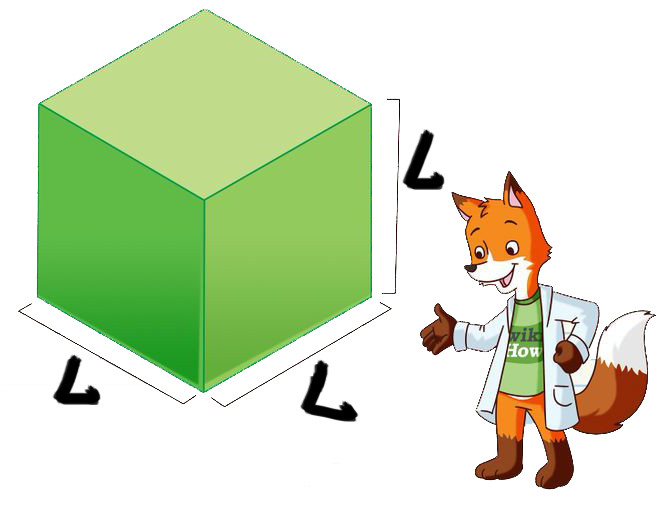
\includegraphics[width=0.5\linewidth]{fig/L1/cube}
		\caption{Formulation of the problem}
		\label{fig:cube}
	\end{figure}

	Solution of \eqref{eq:forA} may be written as the sum of all eigen solutions (each of it is a plane wave) in respect that boundary conditions are periodic:
	\begin{equation}
		\vec{A}(\vec{r},t) = \sum_{\vec{k}} \vec{A}_{\vec{k}}(t) e^{i \vec{k} \vec{r}}, \qquad k_{\alpha} = \frac{2 \pi n_{\alpha}}{L}, \quad \alpha = x,y,z.
	\end{equation}
	%Where $\vec{n}$ --- a unit vector. 
\textcolor{red}{Where $n_{\alpha}$ --- is an integer number.}
As waves are plane then we should write
	\begin{equation}
		\vec{A}_{\vec{k}}(t) = \vec{c}_{\vec{k}} e^{-i \omega_{\vec{k}}t} + \vec{c}_{-\vec{k}}^* e^{i \omega_{\vec{k}}t},
	\end{equation}
	where $\omega_{\vec{k}} = c k = c\sqrt{k_x^2 + k_y^2 + k_z^2}$. 
Let us make a remark: $\vec{A}_{\vec{k}} \in \mathbb{R}$, \textcolor{red}{so
\begin{equation}\label{kminsk}
		\vec{A}_{\vec{k}}(t)=\vec{A}_{\vec{k}}^*(t) = \vec{c}_{-\vec{k}} e^{-i \omega_{\vec{k}}t}+ \vec{c}_{\vec{k}}^* e^{i \omega_{\vec{k}}t}=\vec{A}_{\vec{-k}}(t),
	\end{equation} }.
	The Lorentz gauge leads to the fact that \textit{waves are transverse}:
	\begin{equation}
		\Div \vec{A} = 0 \quad \to \quad \sum \vec{k} \vec{A}_{\vec{k}} e^{i \vec{k} \vec{r}} = 0 \quad \Longleftrightarrow \quad \boxed{\vec{A}_{\vec{k}}(t) \cdot \vec{k} = 0.}
	\end{equation} 
	
	Consider a wave with wave vector $\vec{k}$. According to Maxwell equations, there are two independent polarizations, so we introduce two transverse polarization vectors $\vec{e}_{\vec{k}1}; \vec{e}_{\vec{k}2}$. Three vectors $(\vec{e}_{\vec{k}1}; \vec{e}_{\vec{k}2}; \vec{k}/k)$ form a right-handed orthonormal basis which implies:
	\begin{equation}
		\begin{matrix}
			\vec{k} \cdot \vec{e}_{\vec{k}s} = 0, && \vecmult{\vec{e}_{\vec{k}1}}{\vec{e}_{\vec{k}2}} = \vec{k}/k, \\ \\
			\vec{e}_{\vec{k}s} \cdot \vec{e}_{\vec{k}s'} = \delta_{ss'}, && \vec{c}_{\vec{k}} = \sum_s c_{\vec{k}s} \vec{e}_{\vec{k}s}.
		\end{matrix}
	\end{equation}
	After that we can rewrite decomposition of $\vec{A}$ as
	\begin{multline}
		\vec{A} = \sum_{\vec{k},s} \tilde{A}_{\vec{k}} \left( c_{\vec{k}s} \vec{e}_{\vec{k}s} e^{-i \omega_{\vec{k}} t} + c^*_{-\vec{k}s} \vec{e}^*_{-\vec{k}s}  e^{i \omega_{\vec{k}} t} \right) \cdot e^{i \vec{k} \vec{r}} = \\
		= \left/ \text{inverse 2nd sum \textcolor{red}{using \eqref{kminsk}}: } (-k) \to k \right/ =\sum_{\vec{k},s} \tilde{A}_{\vec{k}} \left( u_{\vec{k}s}(t) \vec{e}_{\vec{k}s} e^{i \vec{k} \vec{r}} + u^*_{\vec{k}s}(t) \vec{e}^*_{\vec{k}s}  e^{-i \vec{k} \vec{r}} \right),
	\end{multline}
	where $u_{\vec{k}s}(t) = c_{\vec{k}s} e^{-i \omega_{\vec{k}} t}$. Now we can write fields
	\begin{equation}
		\vec{E} = -\frac{1}{c} \parder{\vec{A}}{t} = \frac{i}{c} \sum_{\vec{k},s} \tilde{A}_{\vec{k}} \omega_{\vec{k}} \left( u_{\vec{k}s}(t) \vec{e}_{\vec{k}s} e^{i \vec{k} \vec{r}} - u^*_{\vec{k}s}(t) \vec{e}^*_{\vec{k}s}  e^{-i \vec{k} \vec{r}} \right),
	\end{equation}
	\begin{equation}
		\vec{H} = \Rot \vec{A} = i \sum_{\vec{k},s} \tilde{A}_{\vec{k}} \left( u_{\vec{k}s} \left[ \vec{k} \times \vec{e}_{\vec{k}s} \right] e^{i \vec{k} \vec{r}} - u^*_{\vec{k}s} \left[ \vec{k} \times \vec{e}^*_{\vec{k}s} \right] e^{-i \vec{k} \vec{r}} \right).
	\end{equation}
	
	The energy of EM field
	\begin{equation}
		\mathscr{H} = \frac{1}{8 \pi} \int \left(\vec{H}^2 + \vec{E}^2 \right) dV.
	\end{equation} 
	\textit{Remark:} there is no averaging over time!
	
	To make next calculations easier, let us notice that
	\begin{eqnarray}
		\int \limits_{L^3} e^{i (\vec{k} - \vec{k}')\vec{r}} dV = L^3 \delta_{\vec{k}\vec{k}'}.
	\end{eqnarray}
	This feature vanish the $\sum_{\vec{k}}$. Besides, it's convenient to notice that
	\begin{equation}
		\vec{e}_{\vec{k}s}^* \cdot \vec{e}_{\vec{k}s'} = \delta_{ss'} \qquad \to \qquad
		\left[ \vec{k} \times \vec{e}_{\vec{k}s}^* \right] \cdot \left[ \vec{k} \times \vec{e}_{\vec{k}s'} \right] = k^2 \delta_{ss'}.
	\end{equation}
	Then we get
	\begin{equation}
		\mathscr{H} = \frac{L^3}{8 \pi}\textcolor{red}{2} \sum_{\vec{k},s} \tilde{A}_{\vec{k}}^2 \Bigg( \underbrace{\frac{\omega_{\vec{k}}^2}{c^2} \left| u_{\vec{k}s} \right|^2}_{\hookrightarrow E^2} + \underbrace{k^2 \left| u_{\vec{k}s} \right|^2}_{\hookrightarrow H^2}  \Bigg), \qquad k^2 = \frac{\omega_{\vec{k}}^2}{c^2} \text{\ \ (for each mode!)}
	\end{equation}
	\begin{equation}
		\mathscr{H} = \frac{L^3}{\textcolor{red}{2} \pi} \sum_{\vec{k},s} \tilde{A}_{\vec{k}}^2 k^2 \left| u_{\vec{k}s} \right|^2.
	\end{equation}
	Segregation if real and imaginary part of mode can be done by introducing new variables
	\begin{eqnarray}
		q_{\vec{k}s}(t) &=& u_{\vec{k}s}(t) + u^*_{\vec{k}s}(t) , \\
		p_{\vec{k}s}(t) &=& -i \omega_{\vec{k}}  \left( u_{\vec{k}s}(t) - u^*_{\vec{k}s}(t) \right).
	\end{eqnarray}
	It's obvious that
	\begin{equation}
		u_{\vec{k}s}(t) = \frac{1}{2} q_{\vec{k}s}(t) - \frac{1}{2 i \omega} p_{\vec{k}s}(t) \quad \to \quad \left| u_{\vec{k}s} \right|^2 = \frac{1}{4 \omega_{\vec{k}}^2} \left( p^2_{\vec{k}s} + \omega^2_{\vec{k}} q_{\vec{k}s}^2 \right).
	\end{equation}
	The Hamiltonian function will be as follows
	\begin{equation}
		\mathscr{H} = \frac{L^3}{\textcolor{red}{4} \pi c} \sum_{\vec{k},s} \frac{\tilde{A}_{\vec{k}}^2}{2} \left( p^2_{\vec{k}s} + \omega^2_{\vec{k}} q_{\vec{k}s}^2 \right).
	\end{equation}
	Let us boldly put $\tilde{A}_{\vec{k}} = \sqrt{\textcolor{red}{4} \pi c^2/L^3}$, then finally
	\begin{equation}
		\mathscr{H} = \sum_{\vec{k},s}  \left( \frac{p^2_{\vec{k}s}}{2}+ \frac{\omega^2_{\vec{k}} q_{\vec{k}s}^2}{2} \right).
	\end{equation}
	
	If we can write full energy of the system like $\mathscr{H} \sim p^2/2 + \omega^2 q^2/2$, then it means this system can be quantize.  So next, we  \textit{quantize fields}. First of all we need to move to operators by doing
	\begin{equation}
		\begin{cases}
		q_{\vec{k}s} \to \hat{q}_{\vec{k}s}, \\
		p_{\vec{k}s} \to \hat{p}_{\vec{k}s}.
		\end{cases}
	\end{equation}
	After that our Hamiltonian function will transform to Mr. Hamiltonian. 
	Besides, coordinate and impulse operator must obey next commutation relations:
	\begin{equation}
		\left[\hat{q}_{\vec{k}s} ; \hat{p}_{\vec{k}'s'} \right] = i \hbar \delta^{(3)}_{\vec{k}\vec{k}'} \delta_{ss'},
		\label{eq:con1}
	\end{equation} 
	\begin{equation}
		\left[\hat{q}_{\vec{k}s} ; \hat{q}_{\vec{k}'s'} \right] = \left[\hat{p}_{\vec{k}s} ; \hat{p}_{\vec{k}'s'} \right] = 0.
		\label{eq:con2}
	\end{equation}
	Moreover, this operators must be Hermitian because $\mathscr{H}$ stands for real energy which we can measure. Therefore
	\begin{equation}
		\hat{q}_{\vec{k}s} = \hat{q}^{\dagger}_{\vec{k}s}, \qquad \hat{p}_{\vec{k}s} = \hat{p}^{\dagger}_{\vec{k}s}.
		\label{eq:con3}
	\end{equation}
	Relations \eqref{eq:con1}, \eqref{eq:con2} and \eqref{eq:con3} impose conditions for $\hat{q}_{\vec{k}s}$ and $\hat{p}_{\vec{k}s}$.
	Hereafter we can introduce ladder operators:
	\begin{eqnarray}
		\hat{a}_{\vec{k}s}(t) &=& \dfrac{1}{\sqrt{2 \hbar \omega}} \left( \omega \hat{q}_{\vec{k}s} + i \hat{p}_{\vec{k}s} \right), \\ \nonumber \\
		\hat{a}^{\dagger}_{\vec{k}s}(t) &=& \dfrac{1}{\sqrt{2 \hbar \omega}} \left( \omega \hat{q}_{\vec{k}s} - i \hat{p}_{\vec{k}s} \right).
	\end{eqnarray}
	This leads to the useful representation of $\hat{q}_{\vec{k}s}$ and $\hat{p}_{\vec{k}s}$:
	\begin{eqnarray}
		\hat{q}_{\vec{k}s}(t) &=& \sqrt{\dfrac{\hbar}{2 \omega}} \left( \hat{a}^{\dagger}_{\vec{k}s} +  \hat{a}_{\vec{k}s} \right), \\ \nonumber \\
		\hat{p}_{\vec{k}s}(t) &=& i \sqrt{\dfrac{\hbar \omega}{2}} \left( \hat{a}^{\dagger}_{\vec{k}s} -  \hat{a}_{\vec{k}s} \right).
	\end{eqnarray}
	
	Commutation relations can be easily derived from consideration $\left[ \hat{q}_{\vec{k}s} ; \hat{p}_{\vec{k}s} \right]$ in the repre-sentation  of ladder operators and using \eqref{eq:con1} and \eqref{eq:con2}. So we get
	\begin{equation}
		\left[ \hat{a}_{\vec{k},s} ; \hat{a}^{\dagger}_{\vec{k}',s'} \right] = \delta^{(3)}_{\vec{k}\vec{k}'} \delta_{ss'}.
	\end{equation}
	
	Easy to show that Hamiltonian can be written as follows
	\begin{equation}
		\hat{\mathscr{H}} = \sum_{\vec{k},s} \hbar \omega_{\vec{k}} \left[ \hat{a}^{\dagger}_{\vec{k},s} \hat{a}_{\vec{k},s} + \frac{1}{2} \right].
	\end{equation}
	
	
	\section{Coherent states}

\begin{otherlanguage}{russian}
	\epigraph{Из всех родов, видов, сортов и пород людей самая гнусная --- теоретики.}{\sout{А. Куприн} \\Д. А. Байко}
\end{otherlanguage}

\subsection{Eigenfunction}

Let us consider singlemode field.
%only one emission mode
We will be looking for those photons' states which allow us to get more classical world outlook. In particular we want $\hat{\vec{E}}$ be measurable. So, at first, we need to find eigenfunction of annihilation operator $\hat{a}$.

The first naive idea that may come to mind is to check Fock states. Let's look closer at matrix elements
\begin{equation}
	\bra{m} \hat{a} \ket{n} =
	\begin{pmatrix}
		0 & \sqrt{1} & 0 &  \cdots  & 0 & \cdots \\
		0 & 0 & \sqrt{2} &  \cdots & 0 & \cdots \\
		\vdots & \vdots & \ddots & \ddots & \vdots  & \cdots \\
		0 & \vdots & \cdots & 0 & \sqrt{n} & \cdots \\
		\vdots & \vdots & \vdots & \vdots & \vdots & \ddots\\
	\end{pmatrix}.
\end{equation}
Now it's clear that $\ket{n}$ is not a eigenfunction because there are no elements on the main diagonal.

The ordinary procedure to find eigenfunction is the following. $\ket{\alpha}$ should satisfy
\begin{equation}
	\hat{a} \ket{\alpha} = \alpha \ket{\alpha}.
\end{equation}
where $\alpha$ --- eigenvalue.
Fock states form full basis, so we can write
\begin{equation}
	\ket{\alpha} = \sum_{n=0}^{\infty} c_n \ket{n},
\end{equation}
then
\begin{equation}
	\hat{a} \ket{\alpha} = \sum_{n=0}^{\infty} c_n \hat{a} \ket{n} = \sum_{n=0}^{\infty} c_n \sqrt{n} \ket{n-1} = \sum_{n=0}^{\infty} \sqrt{n+1} \ket{n} = \alpha \sum_{n=0}^{\infty} c_n \ket{n},
\end{equation}
which gives the recurrent relation
\begin{equation}
	c_{n+1} \sqrt{n+1} = c_n \alpha \qquad \to \qquad c_n = \frac{\alpha^n}{\sqrt{n!}} c_0 \qquad \to \qquad \ket{\alpha} = c_0 \sum_{n=0}^{\infty} \frac{\alpha^n}{\sqrt{n!}} \ket{n}.
\end{equation}
The constant $c_0$ can be found from the normalization condition:
\begin{equation}
	\braket{\alpha}{\alpha} = 1 \quad \to \quad 1 = \left|c_0\right|^2 \sum_{n,m = 0}^{\infty} \frac{\left( \alpha^* \right)^m \alpha^n}{\sqrt{m!n!}} \underbrace{\braket{m}{n}}_{\hookrightarrow  \delta_{mn}} = \left|c_0\right|^2 \sum_{n = 0}^{\infty} \frac{\left|\alpha\right|^2}{n!},
\end{equation}
\begin{equation}
	c_0 = e^{- \left|\alpha\right|^2/2} e^{i \varphi}
\end{equation}
and finally
\begin{equation}
	\boxed{\ket{\alpha} = e^{- \left|\alpha\right|^2/2} e^{i \varphi} \sum_{n = 0}^{\infty} \frac{\alpha^n}{\sqrt{n!}} \ket{n}.}
\end{equation}
\textit{Remark:} usually phase $\varphi$ is neglected.

\begin{testexample}[How many photons are in coherent state?]
	%\textcolor{red}{(UNCOMMENT THIS LATER! (see source))} \\
	By definition
	\begin{equation}
	\overline{n} = \bra{\alpha} \hat{a}^{\dagger} \hat{a} \ket{\alpha}.
	\end{equation}
	And since
	\begin{eqnarray}
	\hat{a} \ket{\alpha} &=& \alpha \ket{\alpha}, \\
	\bra{\alpha} \hat{a}^{\dagger}  &=& \alpha^* \bra{\alpha},
	\end{eqnarray}
	then
	\begin{equation}
	\overline{n} = \left| \alpha \right|^2.
	\end{equation}
\end{testexample}

Another important thing to calculate. Let us find the probability of $n$ photons be in $\ket{\alpha}$ state:
\begin{equation}
	p_n = \left| \braket{n}{\alpha} \right|^2 = e^{- \left|\alpha\right|^2} \frac{\left|\alpha\right|^{2n}}{n!}.
\end{equation}
Here we obtained the Poisson distribution with dispersion $\sigma = \left|\alpha\right|^2$ (fig \ref{fig:2_1}).
\begin{figure}
	\centering
	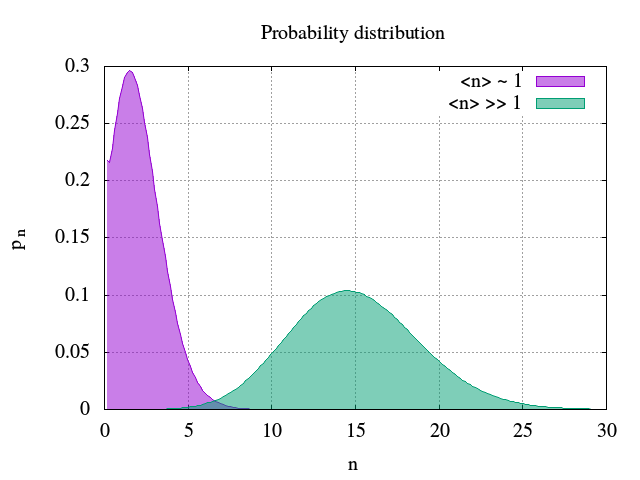
\includegraphics[width=0.7\linewidth]{fig/L2/2_1}
	\caption{Probability distribution for coherent state}
	\label{fig:2_1}
\end{figure}




\begin{hw}[Deadline: 6th of November]
	\addcontentsline{toc}{subsubsection}{Homework}
	\begin{enumerate}
	\item (3 pt) Construct the eigenfunction of the creation operator  $\hat a^{+}|\beta \rangle=\beta|\beta \rangle$.
	
	
	\item (4 pt) Find the eigenfunctions of a coherent state $|\alpha \rangle$ in  the \textbf{position} space (either analytically or numerically).
	
	
	\end{enumerate}
	
	
	{\bf NB:} For solving these problems  you will require the Baker-Campbell-Hausdorff  relations:
	\begin{itemize}
	\item $e^{\hat A+\hat B}=e^{\hat A}e^{\hat B}e^{-\frac{1}{2}[\hat A, \hat B]}$,\ \  if\  $[\hat A,[\hat A,\hat B]]=[\hat B,[\hat B,\hat A]]=[\hat B,[\hat A,\hat B]]=0$
	\item $e^{i\hat A}\hat Be^{-i\hat A} = \hat B + [i\hat A,\hat B] + \dfrac{[i\hat A,[i\hat A,\hat B]]}{2!} + ...$
	\end{itemize}
\end{hw}


\subsection{Orthogonality}

Are coherent states orthogonal or not? Lets find out:
\begin{equation}
	\braket{\alpha'}{\alpha} = e^{- \left|\alpha\right|^2/2} e^{- \left|\alpha'\right|^2/2} \sum \frac{( \accentset{\ast}{\alpha}' )^n \alpha^n}{n!} = e^{-\frac{1}{2} \left|\alpha\right|^2} e^{-\frac{1}{2} \left|\alpha'\right|^2 } e^{\accentset{\ast}{\alpha}' \alpha} \neq 0,
\end{equation}
\begin{equation}
	\left|\braket{\alpha'}{\alpha}\right|^2 = e^{- \left| \alpha - \alpha' \right|^2}.
\end{equation}



\begin{testexample}[If you really want, you can consider coherent states as orthogonal ones!]
	%\textcolor{red}{(UNCOMMENT THIS LATER! (see source))}
	\begin{equation}
	\begin{matrix}
	\ket{\alpha} &=& \ket{3+4i} \\
	\ket{\alpha'} &=& \ket{4+3i} \\
	\end{matrix}
	\quad \to \quad \left|\braket{\alpha'}{\alpha}\right|^2 = e^{-2} \approx 0.1
	\end{equation}
	\begin{equation}
	\begin{matrix}
	\ket{\alpha} &=& \ket{3+4i} \\
	\ket{\alpha'} &=& \ket{-4-3i} \\
	\end{matrix}
	\quad \to \quad \left|\braket{\alpha'}{\alpha}\right|^2  = e^{-98}.
	\end{equation}
	This is a VERY small value!
\end{testexample}

\begin{hw}[Fullness of coherent states.]
Let the reader check the fullness of coherent states. In other words needless to show that
\begin{equation}
	\mathbb{1} = \frac{1}{\pi} \int \limits_{\mathbb{C}} d^2 \alpha \ket{\alpha} \bra{\alpha}.
\end{equation}
\textit{Hint:} for Fock states $\sum_{n=0}^{\infty} \ket{n} \bra{n} = 1$.\\
\textit{Remark:} actually coherent states have the property of overfullness in the sense these states form a basis, but not orthogonal, and one may be expressed with the others.
\end{hw}

Consider the following singlemode field. So this
\begin{equation}
	\hat{\vec{E}} = \sum_{\vec{k},s} \varepsilon_{\vec{k}s} \left( \hat{a}_{\vec{k}s} \vec{e}_{\vec{k}s} e^{i \vec{k} \vec{r} - i \omega_{\vec{k}}t} + \text{ e. c.} \right)
\end{equation}
will be simplified to
\begin{equation}
	\hat{\vec{E}} = \varepsilon \left( \hat{a} \vec{e} e^{i \vec{k} \vec{r} - \omega t} + \text{ e. c.}\right).
\end{equation}
Mean value
\begin{equation}
	\vec{E} = \bra{\alpha} \hat{\vec{E}} \ket{\alpha} = \varepsilon \alpha \vec{e} e^{i \vec{k} \vec{r} - \omega t} + \text{ c. c.} \myeq \vec{E}_+(\vec{r},t) + \vec{E}_-(\vec{r},t).
\end{equation}
The amplitude is defined by $\alpha$:
\begin{equation}
	\vec{E}_+ = E_+ \vec{e} e^{i \vec{k} \vec{r} - \omega t}, \qquad E_+ = \alpha \varepsilon, \qquad \varepsilon = \sqrt{\frac{2 \pi \hbar}{V \omega}}.
\end{equation}
The intensity is proportional to
\begin{equation}
	I_+ \propto \left|E_+\right|^2 = \varepsilon^2 \left|\alpha\right|^2 = \varepsilon^2 \overline{n}.
\end{equation}
From here it is clear that $\varepsilon^2$ stands for the square of electric field amplitude per one photon. Often it is convenient to pick out a phase
\begin{equation}
	E_+ = \varepsilon \left|\alpha\right| e^{i \varphi}.
\end{equation}

Another property of coherent states. Since
\begin{equation}
	\hat{a} \ket{\alpha} = \alpha \ket{\alpha},
\end{equation}
then number of photons in the system does not change! {\textcolor{red}{WAT}}


\begin{hw}[Deadline: 6th of November]
	\addcontentsline{toc}{subsubsection}{Homework}
	
	\begin{enumerate}
	\item (3 pt) Prove the overcompleteness of coherent states:
	$$
	\mathbf{1}=\int_\mathbb{ C} |\alpha\rangle \langle \alpha| \frac{d^{2}\alpha}{\pi}
	$$
	\end{enumerate}


	{\bf NB:} For solving these problems  you will require the Baker-Campbell-Hausdorff  relations:
	\begin{itemize}
	\item $e^{\hat A+\hat B}=e^{\hat A}e^{\hat B}e^{-\frac{1}{2}[\hat A, \hat B]}$,\ \  if\  $[\hat A,[\hat A,\hat B]]=[\hat B,[\hat B,\hat A]]=[\hat B,[\hat A,\hat B]]=0$
	\item $e^{i\hat A}\hat Be^{-i\hat A} = \hat B + [i\hat A,\hat B] + \dfrac{[i\hat A,[i\hat A,\hat B]]}{2!} + ...$
	\end{itemize}

\end{hw}


\subsection{Fluctuations}

Let look at Fock states again. To draw a phase plane we need to remember that
\begin{equation}
	\hat{p} = i \sqrt{\frac{\hbar \omega}{2}} \left( \hat{a}^{\dagger} - \hat{a} \right), \qquad \hat{q} = \sqrt{\frac{\hbar}{2 \omega}}\left( \hat{a}^{\dagger} + \hat{a} \right).
\end{equation}
To find fluctuations let us compute
\begin{equation}
	\overline{p} = \bra{n} \hat{p} \ket{n} = 0, \qquad \overline{q} = \bra{n} \hat{q} \ket{n} = 0
\end{equation}
and
\begin{eqnarray}
	\overline{p^2} = \bra{n} \hat{p}^2 \ket{n} = \frac{\hbar \omega}{2} \left( 2n+1 \right), \\
	\overline{q^2} = \bra{n} \hat{q}^2 \ket{n} = \frac{\hbar}{2 \omega} \left( 2n+1 \right).
\end{eqnarray}
So we have
\begin{equation}
	\Delta p = \sqrt{\overline{p^2} - \overline{p}^2} = \sqrt{\frac{\hbar \omega}{2}} \sqrt{\left( 2n+1 \right)},
\end{equation}
\begin{equation}
	\Delta q = \sqrt{\overline{q^2} - \overline{q}^2} = \sqrt{\frac{\hbar }{2\omega}} \sqrt{\left( 2n+1 \right)}.
\end{equation}
Now we can rewrite the uncertainty principle as following
\begin{equation}
	\Delta p \Delta q = \frac{\hbar}{2} \left(2n+1\right).
\end{equation}

\begin{figure}
	\centering
	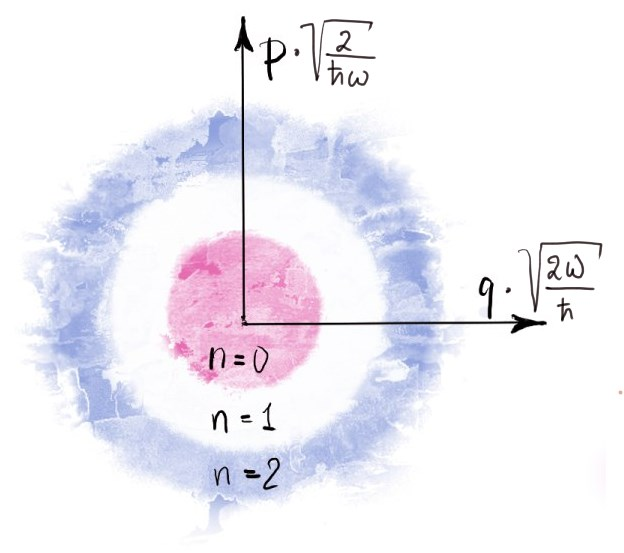
\includegraphics[width=0.4\linewidth]{fig/L2/fluc2}
	\caption{Fluctuations of the Fock states}
	\label{fig:fluc}
\end{figure}

Now let us find the thing for coherent states:
\begin{equation}
	\overline{p} = \bra{\alpha} \hat{p} \ket{\alpha} = i \sqrt{\frac{\hbar \omega}{2}} \left( \alpha^* - \alpha \right) = 2 \sqrt{\frac{\hbar \omega}{2}} \Im \left\{ \alpha \right\},
\end{equation}
\begin{equation}
	\overline{q} = 2 \sqrt{\frac{\hbar }{2\omega}} \Re \left\{\alpha \right\},
\end{equation}
\begin{equation}
	\overline{p^2} = - \frac{\hbar \omega}{2} \bra{\alpha} \hat{a}^{\dagger 2} - \hat{a}^{\dagger} \hat{a} - \hat{a} \hat{a}^{\dagger} + \hat{a}^2  \ket{\alpha} = \frac{\hbar \omega}{2} \left( 4 \Im \left\{ \alpha \right\} + 1\right),
\end{equation}
\begin{equation}
	\overline{q^2} = \frac{\hbar}{2 \omega} \left( 4 \Re \left\{ \alpha \right\} + 1\right).
\end{equation}
Then
\begin{equation}
	\Delta p_{\alpha} = \sqrt{\frac{\hbar \omega}{2} \left[ 4 \Im \left\{ \alpha \right\} + 1 - 4 \Im \left\{ \alpha \right\} \right]^{1/2}} = \frac{\hbar \omega}{2}, \qquad \Delta q_{\alpha} = \frac{\hbar}{2 \omega}.
\end{equation}
The uncertainty relation will be
\begin{equation}
	\boxed{\Delta p_{\alpha} \Delta q_{\alpha} = \frac{\hbar}{2} \quad \slashed{\sim} \quad  \alpha.}
\end{equation}
Here we see that $\Delta p_{\alpha} \Delta q_{\alpha}$ relation does not depend on $\alpha$! In fact we obtained a shifted ground Fock state (fig \ref{fig:shifted_Fock}).

\begin{figure}
	\centering
	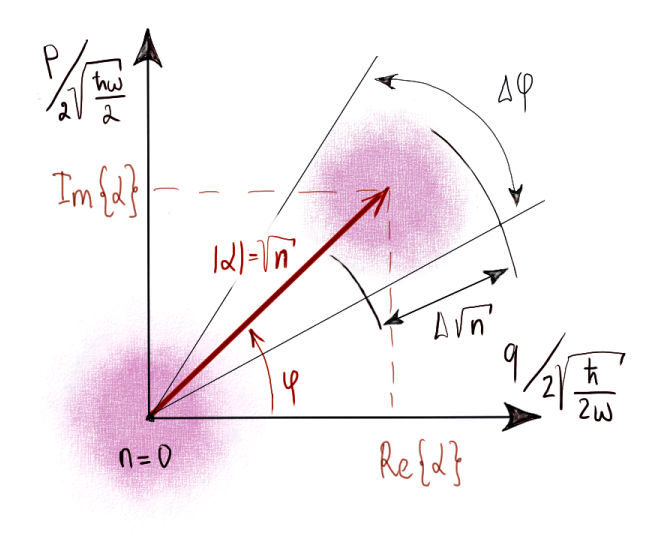
\includegraphics[width=0.6\linewidth]{fig/L2/shifted_Fock1}
	\caption{Shifted Fock states}
	\label{fig:shifted_Fock}
\end{figure}

It conveys the suggestion that a linear operator $\hat{D}(\alpha)$ exist which does this shifting (so-termed \textit{the displacement operator}). In other words
\begin{equation}
	\ket{\alpha} = \hat{D} (\alpha) \ket{0},
\end{equation}
\begin{equation}
	e^{-|\alpha|^2/2} \sum_{n=0}^{\infty} \frac{\alpha^n}{\sqrt{n!}} \ket{n}  = \hat{D} (\alpha) \ket{0},
\end{equation}
and since $\ket{n} = \frac{\left( \hat{a}^{\dagger} \right)^n}{\sqrt{n!}} \ket{0}$, so
\begin{equation}
	D(\alpha) = e^{-|\alpha|^2/2} e^{\alpha \hat{a}^{\dagger}} e^{- \alpha^* \hat{a}}.
\end{equation}
\textit{Remark:} factor $e^{- \alpha^* \hat{a}}$ does not change the result (because $e^{- \alpha^* \hat{a}} \ket{0} = \ket{0}$), but gives some additional properties to the $\hat{D}(\alpha)$:
\begin{enumerate}
	\item Using the Hausdorff relation we can get an alternative from of the displacement operator:
	\begin{equation}
		\hat{D}(\alpha) = e^{\alpha \hat{a}^{\dagger} - \alpha^* \hat{a}}.
	\end{equation}
	\item The displacement operator is a unitary operator. It means that $\hat{D}(\alpha) \hat{D}^{\dagger}(\alpha) = \hat{D}^{\dagger}(\alpha) \hat{D}(\alpha) = \hat{\mathbb{1}}$.
	\item Since $\hat{D}^{\dagger}(\alpha) = \hat{D}(-\alpha)$, the hermitian conjugate of the displacement operator can also be interpreted as a displacement of opposite magnitude.
	\item Following relations hold:
	\begin{eqnarray}
		\hat{D}^{\dagger} (\alpha) \hat{a} \hat{D} (\alpha) &=& \hat{a} + \alpha, \\
		\hat{D} (\alpha) \hat{a} \hat{D}^{\dagger} (\alpha) &=& \hat{a} - \alpha, \\
		\hat{D} (\alpha) \hat{D} (\beta) &=& e^{(\alpha \beta^* - \alpha^* \beta)/2} \hat{D} (\alpha + \beta).
	\end{eqnarray}
\end{enumerate}

In many practical cases a natural question appears: \textit{is it possible to overcome the limit of} $\Delta p_{\alpha} \Delta q_{\alpha} = \frac{\hbar}{2}$ \textit{to get more accurate measurements?}

\begin{hw}[Deadline: 6th of November]
	\addcontentsline{toc}{subsubsection}{Homework}


	\begin{enumerate}
	
	\item (2 pts) Show that the  operator $D(\alpha)=\exp(\alpha\hat{a^\dagger}-\alpha^*\hat{a})$ { displaces} the creation operator by proving the following relations:
	%$$
	%1) D(\alpha)|0\rangle=|\alpha\rangle
	%$$
	$$
	D(\alpha)\hat{a}D(\alpha)^{-1}=\hat{a}-\alpha
	$$
	\item (6 pts) Compute the matrix elements $\langle m| \hat{D}(\alpha)|n\rangle$ of the displacement operator in Fock's basis. Express the result in terms of associated Laguerre polynomials.
	
	\end{enumerate}
	
	
	{\bf NB:} For solving these problems  you will require the Baker-Campbell-Hausdorff  relations:
	\begin{itemize}
	\item $e^{\hat A+\hat B}=e^{\hat A}e^{\hat B}e^{-\frac{1}{2}[\hat A, \hat B]}$,\ \  if\  $[\hat A,[\hat A,\hat B]]=[\hat B,[\hat B,\hat A]]=[\hat B,[\hat A,\hat B]]=0$
	\item $e^{i\hat A}\hat Be^{-i\hat A} = \hat B + [i\hat A,\hat B] + \dfrac{[i\hat A,[i\hat A,\hat B]]}{2!} + ...$
	\end{itemize}
\end{hw}

\subsection{Squeezed states or getting the maximum accuracy!}

Sure, we cannot break the uncertainty principle but we can title the balance of scales for ours good. The main idea is to \textit{squeeze} light state, by geometrical meaning should make an oval from the circle (see fig \ref{fig:sheeeeeeit}).

\begin{figure}[h]
	\begin{minipage}{0.5 \linewidth}
		\center{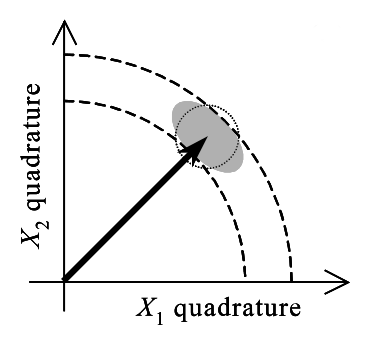
\includegraphics[width=0.7\linewidth]{fig/L2/squeeeeeze_amp} \\ a)}
	\end{minipage}
	\hfill
	\begin{minipage}{0.5 \linewidth}
		\center{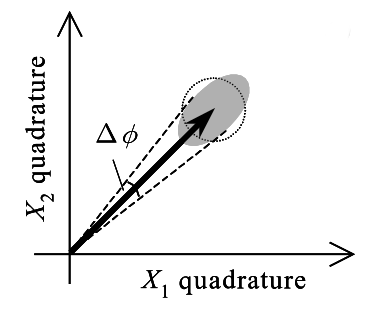
\includegraphics[width=0.7\linewidth]{fig/L2/squeeeeeze_phase} \\ b)}
	\end{minipage}
	\caption{Different light sates on a phase plane: (a) amplitude-squeezed light, (b) phase-squeezed light.}
	\label{fig:sheeeeeeit}
\end{figure}

Let us recall what one property of coherent states
\begin{equation}
	\bra{\alpha} \hat{\vec{E}} \ket{\alpha} = \vec{E} (\vec{r},t).
\end{equation}
From the other hand we have
\begin{equation}
	\bra{n} \hat{\vec{E}} \ket{n} = 0.
\end{equation}
But now if we take into account fluctuations then we get what is shown on fig \ref{fig:noise_MC}. Considering coherent states, lets write a very simplified field time dependence:
\begin{equation}
	E = \varepsilon \left( |\alpha| + \delta \alpha\right) \cos \left[ \omega t + \varphi + \delta \varphi \right],
\end{equation}
where $\delta \alpha$ and $\delta \varphi$ --- fluctuations. For squeezing we will get another picture --- fig \ref{fig:eeeEEeee}.
\begin{figure}
	\centering
	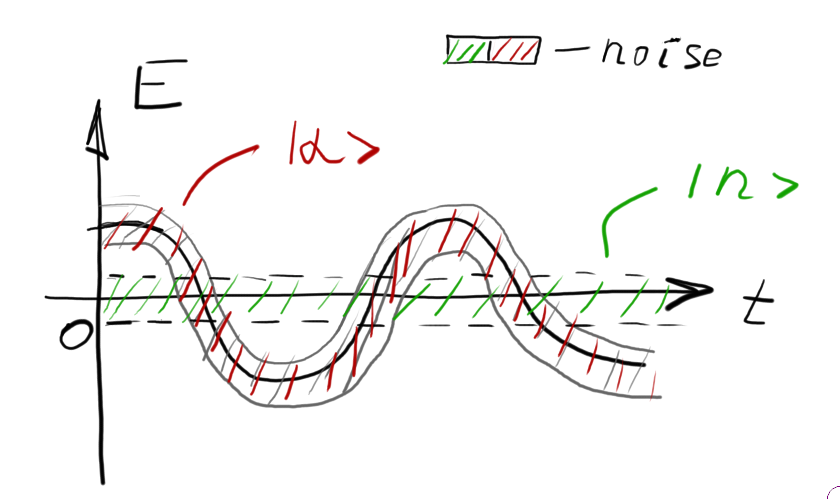
\includegraphics[width=0.65\linewidth]{fig/L2/noise_MC}
	\caption{Field fluctuations for $\ket{\alpha}$ and $\ket{n}$ without squeezing {\textcolor{red}{Here is only ground Fock state shown, next states have greater fluctuations}}}
	\label{fig:noise_MC}
\end{figure}

\begin{figure}
	\centering
	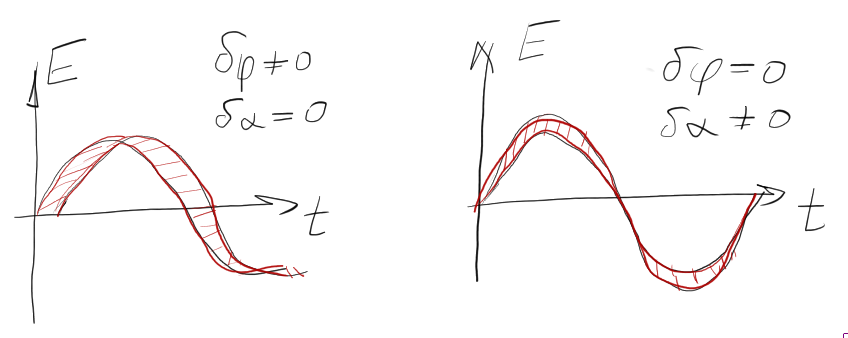
\includegraphics[width=0.7\linewidth]{fig/L2/eeeEEeee}
	\caption{Field fluctuations for squeezed light}
	\label{fig:eeeEEeee}
\end{figure}

To get quantitative and more specific description one can use \textit{the squeeze operator}:
\begin{equation}
	\hat{S} \left( \xi \right) \ket{\alpha} = \ket{\alpha, \xi},
\end{equation}
where $|\xi|$ --- ratio of the main semiaxes of squeezed state, $\arg  \xi $ --- a turning angle.

Here are some helpful properties of the squeeze operator:
\begin{enumerate}
	\item It make be written as following:
	\begin{equation}
		\hat{S} = e^{\xi \hat{a}^{\dagger 2} - \xi^* \hat{a}^2}.
		\label{eq:SS}
	\end{equation}
	\item It is commutative with displacement operator:
	\begin{equation}
		\hat{S} (\xi) \hat{D} (\alpha) \neq  \hat{D} (\alpha) \hat{S} (\xi).
	\end{equation}
\end{enumerate}

Lets draw attention to \eqref{eq:SS}. We can notice that squeeze operator $\hat{S}$ consist of squares of ladder operators ($\sim \hat{a}^{\dagger 2}, \hat{a}^{2}$). It means here we have a generation of second harmonic ($2 \hbar \omega$ instead of $\hbar \omega$). In other words,  from a experimenter's point of view, to get the squeezed state one needs a non-linear optical element with $\chi_2 \neq 0$, so it's polarizability $P = \chi_1 E + \chi_2 E^2$. 



\begin{hw}[Deadline: 6th of November]
	\addcontentsline{toc}{subsubsection}{Homework}

	\begin{enumerate}
		\item (4 pt) {\bfseries Classical squeezing.}\\
		For the problem of a classical harmonic oscillator a general solution can be expressed as $x(t) = c_1 cos\omega_0t + c_2 sin \omega_0t$, where $c_1$ and $c_2$ depend on the  initial conditions. Now consider that you drive this system on a $2\omega_0$ frequency so that $ V(t) = \frac{1}{2}m\omega_0^2x^2\left(1 + \epsilon sin2\omega_0t \right)$ ($\epsilon << 1$). Prove that $c_1(t) = e^{\beta t}$ and $c_2(t) = e^{-\beta t}$ and find $\beta$ using the second Newton's law, the method of  variation of parameters, considering $c_1(t)$ and $c_2(t)$ as slowly varying variables and ignoring fast-oscillating terms.
		
		\item (5 pt) {\bfseries Quantum squeezing.}\\
		Now you know that for squeezing you need to drive your system at $2\omega_0$ frequency. In quantum case it corresponds to the process of parametric down-conversion when you have a strong coherent field (mode $b$) with a frequency $2 \omega_0$ as an input and on the output you have two photons of frequency $\omega_0$ (mode $a$). It can expressed with the following Hamiltonian $\hat H = \hat a^\dagger \hat a^\dagger \hat b + \hat a \hat a \hat b^\dagger$. The corresponding squeezing operator is $\hat S(r) = exp\left[-\frac{r}{2}\left( \hat a^2 - \hat a^{\dagger 2}\right)\right]$, here $r$ describes the strength of squeezing. Compute \\
		$$1) \hat S(r) \hat x \hat S^\dagger (r)$$
		$$2) \hat S(r) \hat p \hat S^\dagger (r)$$
		where $\hat x = \frac{\hat a + \hat a^\dagger}{\sqrt[]{2}}$ and $\hat p = \frac{\hat a - \hat a^\dagger}{\sqrt[]{2}}$.
	\end{enumerate}

	{\bf NB:} For solving these problems  you will require the Baker-Campbell-Hausdorff  relations:
	\begin{itemize}
		\item $e^{\hat A+\hat B}=e^{\hat A}e^{\hat B}e^{-\frac{1}{2}[\hat A, \hat B]}$,\ \  if\  $[\hat A,[\hat A,\hat B]]=[\hat B,[\hat B,\hat A]]=[\hat B,[\hat A,\hat B]]=0$
		\item $e^{i\hat A}\hat Be^{-i\hat A} = \hat B + [i\hat A,\hat B] + \dfrac{[i\hat A,[i\hat A,\hat B]]}{2!} + ...$
	\end{itemize}
\end{hw}

	\section{The coherence of light}

\subsection{Bunching and antibunching of photons}
	
	\section{Atom-field interaction --- semiclassical theory}
\label{sec:atom-field_interaction}

A word \textit{semiclassical} in this context means the following: let us consider a classical electromagnetic field and a <<quantum>> atom. For simplicity let us take two-level system (fig. \ref{fig:2lvl}). Then throw light on this system.
\begin{figure}[h!]
	\centering
	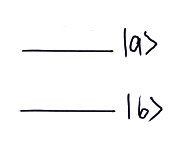
\includegraphics[width=0.4\linewidth]{fig/L4/2lvl}
	\caption{Atom's energy levels }
	\label{fig:2lvl}
\end{figure}

Mr. Hamiltonian is given by
\begin{equation}
	\hat{\mathscr{H}} = \frac{\hat{\vec{p}}^2}{2 m} + \hat{V} (\vec{r}).
\end{equation}
System has eigenstates which are given by equation
\begin{equation}
	\hat{\mathscr{H}} \ket{\psi} = E \ket{\psi}.
\end{equation}
So we have $E_a$ for $\ket{a}$ and $E_b$ for $\ket{b}$. After introducing electromagnetic field we have
\begin{equation}
	\hat{\mathscr{H}} = \frac{(\hat{\vec{p}} - \frac{e}{c} \vec{A})^2}{2m} + \hat{V}(\vec{r}) + e \varphi.
\end{equation}
Potentials are not determined and gauging may take place:
\begin{equation}
	\vec{A} \to \vec{A} + \frac{\hbar c}{e} \nabla \chi, \qquad \varphi \to \varphi - \frac{\hbar c}{e} \parder{\chi}{t}.
\end{equation}
After applying this gauging 
\begin{equation}
	\psi \to \psi e^{i \chi(\vec{r},t)}.
\end{equation}
Let a plane wave is falling 
\begin{equation}
	\vec{A} = \vec{A}_0 e^{i \vec{k}\vec{r} - i \omega t} = \vec{A}_0(t) e^{i \vec{k}\vec{r}}.
\end{equation}
Assume that characteristic scale of the system is such that 
\begin{equation}
	L \ll \lambda
	\label{eq:condition}
\end{equation}
is satisfied. Condition \eqref{eq:condition} is satisfied for lots of quantum systems. 
For example, visible light is $\lambda \sim 400 \div 800 \text{ нм}$, 
characteristic size of an atom is about $10^{-10} \text{ м}$, size of a quantum dot is about $10 \text{ нм}$. 

\begin{figure}[h!]
	\centering
	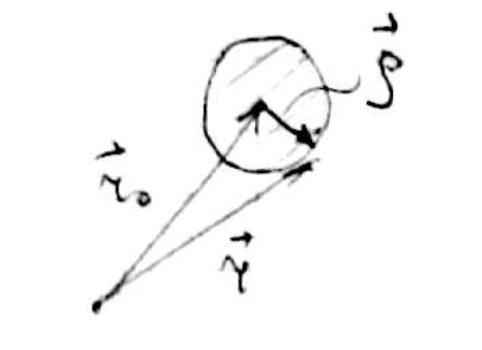
\includegraphics[width=0.4\linewidth]{fig/L4/simply}
	\caption{System}
	\label{fig:simply}
\end{figure}


Using this simplification we can $\vec{r}_0 \to \vec{r}$, where $\vec{r}_0$ is a vector of a centre of the system. More formaly this result may be achieved by expanding $\vec{A}$ near $\vec{r}_0$ in Taylor series:
\begin{equation}
	\vec{A} (\vec{r},t) \approx \vec{A}_0 (t) e^{i \vec{k} \vec{r}_0} \left( 1 + i \vec{k} \bm{\rho} \right) \approx \vec{A}_0 e^{i \vec{k} \vec{r}_0}.
\end{equation} 
So field does not change in space, but in time. Let us choose the system of axes so as to $\vec{r}_0 = 0$. It means that $\vec{A} \approx \vec{A}_0 (t)$. So
\begin{equation}
	\hat{\mathscr{H}} = \frac{1}{2m} \left( \hat{\vec{p}}  - \frac{e}{c} \vec{A}_0(t) \right)^2 + V (\vec{r}) + e \varphi.
\end{equation}
The standard choice it to use Coulomb gauging:
\begin{equation}
	\Div \vec{A} = 0, \qquad \varphi = 0.
\end{equation}
After that, using $\hat{\vec{p}} = -i \hbar \nabla$, we obtain
\begin{equation}
	\hat{\mathscr{H}} = - \frac{\hbar^2}{2m} \left( \nabla - \frac{i e}{\hbar c} \vec{A}_0  \right)^2 + V(\vec{r}).
\end{equation}
Lets introduce a new wave function $\widetilde{\psi} = \psi \underbrace{e^{- i \frac{e}{c \hbar} \vec{A}_0 \vec{r}}}_{\hookrightarrow = u}$. After that, the $ u^{\dagger} \hat{\mathscr{H}} u $ transformation will make an impulse shift.
\begin{equation}
	\hat{\mathscr{H}} \psi = \hat{\mathscr{H}} \widetilde{\psi} e^{i \frac{e}{c \hbar} \vec{A}_0 (t) \vec{r}}.
\end{equation}
We shall call $\vec{g} \myeq \frac{e}{c \hbar} \vec{A}_0 (t)$. After that lets consider
\begin{equation}
	\left( \nabla - i \vec{g} \right) \left( \nabla - i \vec{g} \right) \widetilde{\psi} e^{i \vec{g} \vec{r}} = \\ = \left( \nabla - i \vec{g} \right) \left( \nabla \widetilde{\psi}  \right) e^{i \vec{g} \vec{r}} = \left( \nabla^2 \widetilde{\psi} \right) e^{i \vec{g} \vec{r}}.
\end{equation}
Schroedinger equation gives us
\begin{equation}
	\hat{\mathscr{H}} \psi = i \hbar \parder{\psi}{t},
\end{equation}
\begin{equation}
	\underbrace{\left( - \frac{\hbar^2}{2m} \nabla^2 + V \right)}_{\hat{\mathscr{H}}_0} \widetilde{\psi} (\vec{r},t) = i \hbar \parder{\widetilde{\psi}}{t} - \hbar \vec{r} \cdot \parder{\vec{g}}{t} \widetilde{\psi}.
	\label{eq:tmp143}
\end{equation} 
Lets pay attention to  
\begin{equation}
	\parder{\vec{g}}{t} = \frac{e}{\hbar c} \parder{\vec{A}_0(t)}{t} = - \frac{e}{\hbar} \vec{E}(t).
\end{equation}
Using that we can rewrite \eqref{eq:tmp143} as
\begin{equation}
	\hat{\mathscr{H}}_0 \widetilde{\psi} - e \vec{r} \vec{E} \widetilde{\psi} = i \hbar \parder{\widetilde{\psi}}{t}.
\end{equation}
It's convenient to denote $\hat{\mathscr{H}}_1 \myeq - e \vec{r} \vec{E}$ --- a dipole energy in electric field, so finally
\begin{equation}
	\left( \hat{\mathscr{H}}_0 + \hat{\mathscr{H}}_1 \right) \widetilde{\psi} = i \hbar \parder{\widetilde{\psi}}{t}.
\end{equation}

Let us do an expansion of $\psi$ in eigenstates:
\begin{equation}
	\ket{\psi} = C_a(t) \ket{a} + C_b(t) \ket{b},
\end{equation}
where
\begin{equation}
	\hat{\mathscr{H}}_0 \ket{a} = E_a \ket{a}, \qquad \hat{\mathscr{H}}_0 \ket{b} = E_b \ket{b}.
\end{equation}
Beside $E_a - E_b = \hbar \omega_0$ --- the transition frequency. Let incident field be $\bm{\varepsilon} = \bm{\varepsilon}_0 \cos \omega t$, so $\hat{\mathscr{H}}_1 = - \vec{d} \cdot \bm{\varepsilon}$. Let define initial conditions at moment $t = 0$:
\begin{equation}
	\ket{\psi} \Big|_{t = 0} = \ket{b} \qquad \to \qquad
	\begin{matrix}
		C_a(0) = 0, \\
		C_b(0) = 1.
	\end{matrix}
\end{equation}
So solution is
\begin{equation}
	\left( E_a C_a \ket{a} + E_b C_b \ket{b} \right) - \vec{d} \cdot \bm{\varepsilon} C_a \ket{a} - \vec{d} \cdot \bm{\varepsilon} C_b \ket{b} = i \hbar \dot{C}_a \ket{a} + i \hbar \dot{C}_b \ket{b}.
	\label{eq:tmp150}
\end{equation}
Projections to $\ket{a}$ and $\ket{b}$ gives us 
\begin{equation}
\begin{cases}
	\begin{matrix}
	\bra{a} \cdot \eqref{eq:tmp150}: &\qquad&
	E_a C_a - C_a \bra{a} \vec{d} \cdot \bm{\varepsilon} \ket{a} - C_b \bra{a} \vec{d} \cdot \bm{\varepsilon} \ket{b} = i \hbar \dot{C}_a, \\  \\
	\bra{b} \cdot \eqref{eq:tmp150}: &\qquad& 
	E_b C_b - C_b \bra{b} \vec{d} \cdot \bm{\varepsilon} \ket{b} - C_a \bra{b} \vec{d} \cdot \bm{\varepsilon} \ket{a} = i \hbar \dot{C}_b.
	\end{matrix}
\end{cases}
\label{eq:tmp151}
\end{equation}

Let us assume that field $\bm{\varepsilon}$ is not changing in space, so we can write
\begin{equation}
	\bra{a} \vec{d} \cdot \bm{\varepsilon} \ket{a} = \bra{a} \vec{d} \ket{a} \cdot \bm{\varepsilon}, \qquad 
	\bra{a} \vec{d} \cdot \bm{\varepsilon} \ket{b} = \bra{a} \vec{d} \ket{b} \cdot \bm{\varepsilon}.
\end{equation}
Dipole matrix elements are
\begin{equation}
	\vec{d}_{\alpha \beta} \myeq \bra{\alpha} \vec{d} \ket{\beta} = \int dV \psi_{\alpha}^* (\vec{r}) e \vec{r} \psi_{\beta} (\vec{r}).
\end{equation}
By symmetry considerations it follows  $\left| \vec{d}_{\alpha \alpha} \right| \ll \left| \vec{d}_{\alpha \beta} \right|_{\alpha \neq \beta}$, since usually neighboring states have opposite parity \textcolor{red}{(но это не точно)} and $e \vec{r}$ --- an odd function. Using such approximation (formally just $\vec{d}_{aa}, \vec{d}_{bb} \to 0$ in \eqref{eq:tmp151}) we can write
\begin{equation}
	\begin{cases}
		i \hbar \dot{C}_a = E_a C_a - C_b \vec{d}_{ab} \cdot \bm{\varepsilon}, \\
		i \hbar \dot{C}_b = E_b C_b - C_a \vec{d}_{ba} \cdot \bm{\varepsilon}.
	\end{cases} 
	\qquad \quad \vec{d}_{ba} = \vec{d}_{ab}^*
\end{equation}
Here we can see that if we <<turn off>> the interaction ($\vec{d}_{\alpha \beta} = 0$) states $\ket{a}$ and $\ket{b}$ will be unloosened. If we turn the interaction on transitions will take place. 

To get rid off phase factor we introduce
\begin{equation}
	\widetilde{C}_a (t) \myeq C_a(t) e^{\frac{i}{\hbar}E_a t}, \qquad \widetilde{C}_b (t) \myeq C_b(t) e^{\frac{i}{\hbar}E_a t}.
\end{equation}
After that we have
\begin{equation}
	\begin{cases}
		\dot{\widetilde{C}}_a = \frac{i}{\hbar}\vec{d}_{ab} \cdot \bm{\varepsilon} e^{i \omega_0 t} \widetilde{C}_b(t), \\
		\dot{\widetilde{C}}_b = \frac{i}{\hbar}\vec{d}^*_{ab} \cdot \bm{\varepsilon} e^{-i \omega_0 t} \widetilde{C}_a(t).
	\end{cases} 
\end{equation}

Now we need to apply \textit{rotating wave approximation} (RWA). To understand what is it lets look at 
\begin{equation}
	\bm{\varepsilon}(t) e^{i \omega_0 t} = \bm{\varepsilon}_0 \frac{e^{i \omega t} + e^{- i \omega t}}{2} e^{i \omega_0 t}= \frac{1}{2} \bm{\varepsilon}_0 \left( \underbrace{e^{i(\omega_0 + \omega) t}}_{\text{fast osc.}} + e^{i(\omega_0 - \omega) t} \right).
\end{equation}
Fast oscillating term will lead to a small contribution, so it may be neglected. Leaving only $\sim e^{i (\omega_0 - \omega)t}$ term is called RWA. It's convenient to denote $\Delta \myeq \omega_0 - \omega$, so
\begin{equation}
	\begin{cases}
		\dot{\widetilde{C}}_a = \frac{i}{2\hbar}\vec{d}_{ab} \cdot \bm{\varepsilon}_0 e^{i \Delta t} \widetilde{C}_b(t), \\
		\dot{\widetilde{C}}_b = \frac{i}{2\hbar}\vec{d}^*_{ab} \cdot \bm{\varepsilon}_0 e^{-i \Delta t} \widetilde{C}_a(t).
	\end{cases} 
\end{equation}
Agreed notation is the following
\begin{equation}
	\boxed{\Omega_R \myeq \frac{\left|\vec{d}_{ab} \cdot \bm{\varepsilon}_0\right|}{\hbar}.}
\end{equation}
This is \textit{Rabi frequency}.

To simplify the understanding of our result let us put $\Delta =0$ (resonant excitation) and a specific phase of incident light, so our system will be
\begin{equation}
	\begin{cases}
		\dot{\widetilde{C}}_a = i \frac{\Omega_R}{2} \widetilde{C}_b, \\
		\dot{\widetilde{C}}_b = i \frac{\Omega_R}{2} \widetilde{C}_a.
	\end{cases}
	\label{eq:rabi_system}
\end{equation}
The solution is easy to obtain: $\widetilde{C}_b = \cos \left( \frac{\Omega_R t}{2} \right)$. Only $\left| C_a\right|^2$ and $\left| C_b \right|^2$ have the real physical meaning --- it's the probability of occupation on different states.
\begin{figure}[h!]
	\centering
	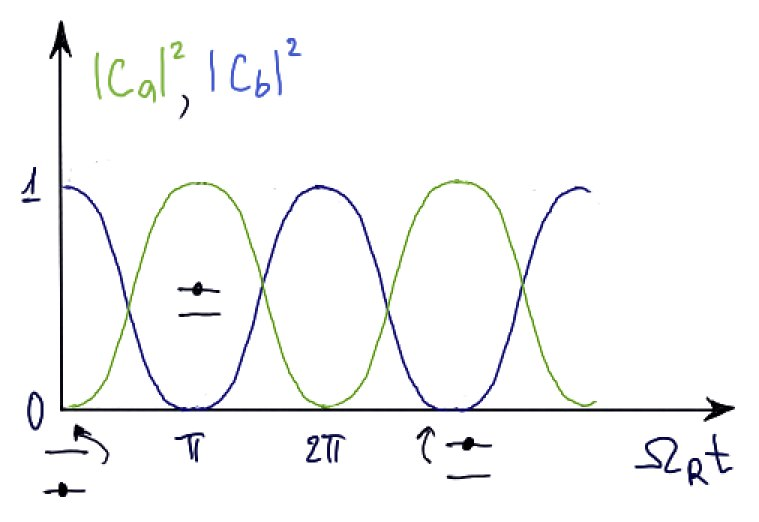
\includegraphics[width=0.65\linewidth]{fig/L4/rabi_osc}
	\caption{Rabi oscillations for two-level system}
	\label{fig:rabiosc}
\end{figure}

Here is a short summary:
\begin{enumerate}
	\item If $\vec{d} \perp \bm{\varepsilon}$ then $\Omega_R = 0$.
	\item To increase Rabi frequency one need to increase the amplitude of incident wave $\left| \bm{\varepsilon} \right|$. 
\end{enumerate}

	
	\section{Density matrix of two energy level system}

\begin{figure}[h!]
	\centering
	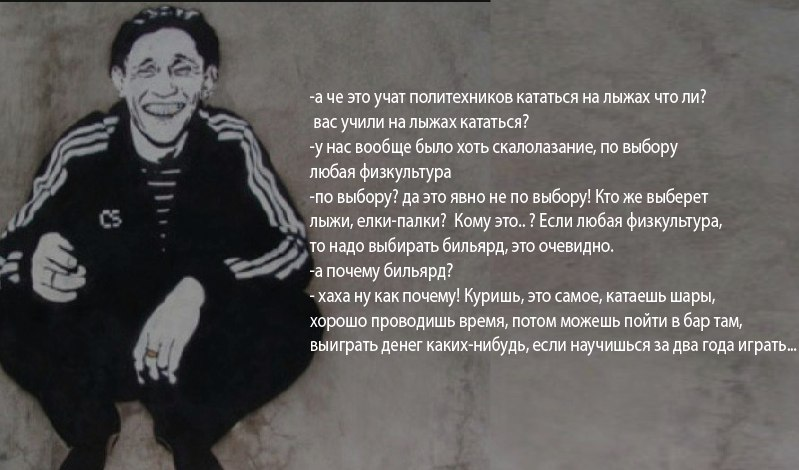
\includegraphics[width=0.8\linewidth]{fig/L4/true_Baiko}
	\caption{The true essence of life choices}
	\label{fig:truebaiko}
\end{figure}

Let consider a two-level system again. In section \ref{sec:atom-field_interaction} we obtained Rabi osculations. Needless to say there weren't any dissipative forces, so turning off the incident field will make the system "freeze" in the last state forever (fig. \ref{fig:turnofffield}). It is obvious that it is not happening in actual truth due to an interaction with immediate media. Adding phenomenological terms to equations for $C_a$ and $C_b$ (e.g. \eqref{eq:rabi_system}) is incorrect because we don't know time dependence of $\ket{\psi(t)}$. The correct way is to use \textit{density matrix formalism}.

\begin{figure}[h!]
	\centering
	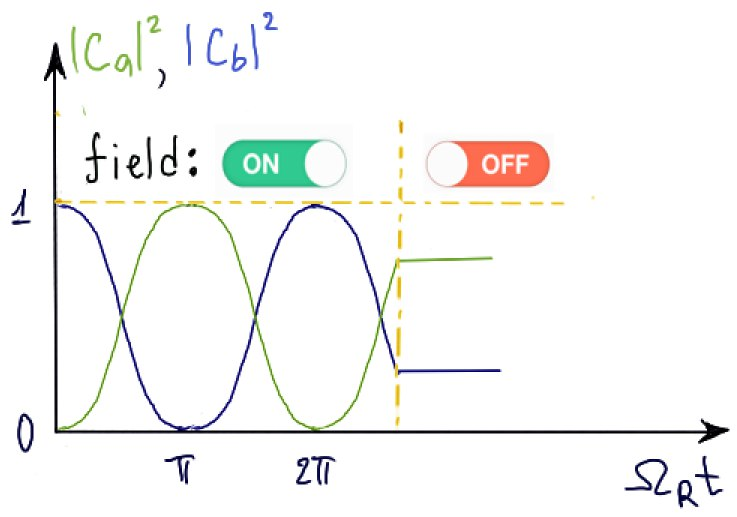
\includegraphics[width=0.65\linewidth]{fig/L5/turn_off_field}
	\caption{Turning the incident field off}
	\label{fig:turnofffield}
\end{figure}


A density matrix is a matrix that describes a quantum system in a mixed state, a statistical ensemble of several quantum states. In other words, density matrix is very useful if we do not know a wave function which contains all the information of the system but we still want to describe our system. There are two possible options (fig. \ref{fig:densmatr}):
\begin{enumerate}
	\item $\ket{\psi_A}$ is known but we need to describe only $B$-system which is intersystem of $A$-system.
	\item $B$ --- is not a conservative system and energy exchanging with reservoir is taking place.
\end{enumerate}
\begin{figure}
	\centering
	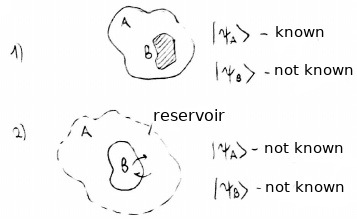
\includegraphics[width=0.7\linewidth]{fig/L5/dens_matr}
	\caption{Possible systems where one need to use density matrix}
	\label{fig:densmatr}
\end{figure}
If $\ket{\psi}$ is known than density matrix is defined by
\begin{equation}
	\boxed{\hat{\rho} = \ket{\psi} \bra{\psi}}
\end{equation}
If we expand to Fock states $\ket{\psi} = \sum C_n \ket{n}$ then 
\begin{equation}
	\hat{\rho} = \sum_{nm} C_n^* C_m \ket{m} \bra{n}.
\end{equation}
Matrix elements --- $\rho_{nm} = C_n^* C_m$.

\begin{testexample}[Density matrix for two-level system.]
	%\textcolor{red}{(UNCOMMENT THIS LATER! (see source))}
	For two-level system we have:
	\begin{equation}
		\ket{\psi} = C_a \ket{a} + C_b \ket{b},
	\end{equation}
	so
	\begin{equation}
		\hat{\rho} = \ket{\psi} \bra{\psi} = 
		\begin{pmatrix}
			\left| C_a (t) \right|^2 & C_a (t) C_b^*(t) \\
			C_b (t) C_a^*(t) & \left| C_b (t) \right|^2
		\end{pmatrix}, \qquad
		\rho_{ij} = \bra{i} \hat{\rho} \ket{j}.
	\end{equation}
\end{testexample}

Mean operator value:
\begin{equation}
	\bar{f} = \bra{\psi} \hat{f} \ket{\psi} \sum_{nm} C_n^* C_m \bra{n} \hat{f} \ket{m} = \sum_{mn} \rho_{nm} f_{nm} = \Tr \left(\hat{\rho} \hat{f}\right).
\end{equation}
\textit{This is the main intended use of density matrix!} Properties:
\begin{enumerate}
	\item Hermiticity: $\hat{\rho}^{\dagger} = \hat{\rho}$.
	\item $\Tr \hat{\rho} = 1 \quad \to \quad$ diagonal elements: $\rho_{mn} = \left| C_n \right|^2$.  Remark: only for pure states!
	\item $]\  \hat{\rho} = \ket{\psi} \bra{\psi} \quad \to \quad \hat{\rho}^2 = \hat{\rho}$. It's easy to show:
	\begin{equation}
		\hat{\rho}^2 = \ket{\psi} \underbrace{\bra{\psi} \ket{\psi}}_{\hookrightarrow = 1} \bra{\psi} = \ket{\psi} \bra{\psi}.
	\end{equation}
	It also means that density matrix of pure state --- projector.
\end{enumerate}

\subsection{Density matrix of mixed state}

Now let us consider a \textit{mixed state}. Let there are lots of systems in different pure states $\ket{\psi_i}$. Let there are $N_i$ particles in $\ket{\psi_i}$, then the whole amount of particles (=systems) is $N = \sum N_i$. The probabily to find any system in $\ket{\psi_i}$ is $\omega_i = \frac{N_i}{N}$. The question we are trying to answer now: how can we find mean operator value?
\begin{equation}
	\bar{f} = \Tr \hat{\rho} \hat{f} = ? \qquad \text{since} \quad \hat{\rho} = ? 
\end{equation}
Scenario is the following:
\begin{enumerate}
	\item Calculation of quantum-average values: $f_i = \bra{\psi_i} \hat{f} \ket{\psi_i}$.
	\item Calculation of classical average values: $\bar{f} = \sum \omega_i f_i$.
\end{enumerate}
So
\begin{multline}
	\bar{f} = \sum \omega_i \bra{\psi_i} \hat{f} \ket{\psi_i} = \sum_i \omega_i \sum_{nm} \underbrace{\left( C_n^i \right)^* C_m}_{\rho_{mn}^i} \underbrace{\bra{n} \hat{f} \ket{m}}_{f_{nm}} = \\
	= \sum_{nm} \sum_i \rho_{mn}^i \omega_i f_{nm} \myeq \Tr \left( \hat{\rho} \hat{f} \right).
\end{multline}
Here we defined density matrix as $\left( \hat{\rho}_{\text{mix}} \right)_{mn} = \sum_i \omega_i \rho_{mn}^i$. Density matrix has a probability meaning:
\begin{equation}
	\hat{\rho}_{\text{mix}} = \sum_i \omega_i \hat{\rho}_i, \qquad \hat{\rho}_i = \ket{\psi_i} \bra{\psi_i}.
\end{equation}
Coefficients $\omega_i$ are defined by \textit{statistical (not quantum!) mechanics} (e.g. Boltzmann distribution).

Remarks:
\begin{enumerate}
	\item $\Tr \hat{\rho}_{\text{mix}} = 1$ by virtue of the fact that $\sum \omega_i = 1$.
	\item $\Tr \hat{\rho}_{\text{mix}}^2 = \sum \omega_i^2 \le 1$. 
	
	Proof:
	\begin{multline}
		\Tr \hat{\rho}_{\text{mix}}^2 = \Tr \sum_{ij} \omega_i \omega_j \sum_{n m} C^*_{m_i} C_{n_i} \ket{n_i} \bra{m_i} \sum_{n' m'} C^*_{m_j'} C_{n_j'} \ket{n_j'} \bra{m_j'} = \\ = \Tr
		\sum_{ij} \omega_i \omega_j \sum_{nmn'm'} C_{m_i}^* C^*_{m_j'}C_{n_i} C_{n_j'} \ket{n_i} \underbrace{\bra{m_i} \ket{n_j'}}_{\hookrightarrow=\delta_{mn'} \delta_{ij}} \bra{m_j'} = \\ = \Tr \sum_i \omega_i^2  \underbrace{\sum_{n'} \left|C_{n'}\right|^2}_{\hookrightarrow = 1} \hat{\rho}_i = \sum_i \omega_i^2.
	\end{multline}
	It means it is not projector anymore! Testing criterion of pureness is introduced by
	\begin{equation}
		\boxed{\mu = \Tr \hat{\rho} - \Tr \hat{\rho}^2 \ge 0}
	\end{equation}
\end{enumerate}

\subsection{Subsystem density matrix}

Let $\hat{f}_A$ is an operator that acts only in subsystem $A$. Now let us ask a question: how to find mean value $\bar{f}_A$?

Subsystem $A$ does not have its own wave function and $\ket{\psi}$ (wave function of $A + B$) does not fall in multiplication of $\ket{\psi_A}$ and $\ket{\psi_B}$. But we can write an expansion in eigenfunctions $\ket{n}$ of subsystem $A$ and $\ket{\alpha}$ of $B$:
\begin{equation}
	\ket{\psi} = \sum_{n \alpha} C_{n \alpha} \ket{n} \ket{\alpha}.
\end{equation}
Now we can write
\begin{multline}
	\bar{f}_A = \bra{\psi} \hat{f}_A \ket{\psi} = \sum_{n \alpha n' \alpha'} C_{n \alpha} C^*_{n' \alpha'} \bra{\alpha'} \overbrace{\bra{n'} \hat{f}_A \ket{n}}^{f_{n' n}} \ket{\alpha} = \\ =
	\sum_{n \alpha n' \alpha'} C_{n \alpha} C^*_{n' \alpha'} f_{n' n} \underbrace{\braket{\alpha'}{\alpha}}_{\hookrightarrow = \delta_{ij}\alpha \alpha'} = \sum_{n n'} \sum_{\alpha}  C_{n \alpha} C^*_{n' \alpha} f_{n' n} = \sum_{n n'} \left( \hat{\rho}_A \right)_{n' n} f_{n' n}.
\end{multline}
Here we denoted
\begin{equation}
	\left( \hat{\rho}_A \right)_{n' n} = \sum_{\alpha}  C_{n \alpha} C^*_{n' \alpha}
\end{equation}
or in other words
\begin{equation}
	\left( \hat{\rho}_A \right)_{n' n} = \sum_{\alpha = \alpha'} \left( \hat{\rho}_{A+B} \right)_{n \alpha n' \alpha'}.
\end{equation}
In the general case:
\begin{equation}
	\boxed{\hat{\rho}_A = \Tr_B \left( \hat{\rho}_{A+B} \right)}
\end{equation}


\subsection{Density matrix for two-level system}

\begin{figure}[h!]
	\centering
	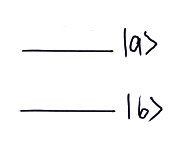
\includegraphics[width=0.25\linewidth]{fig/L4/2lvl}
	\caption{A two-level system}
	\label{fig:2lvl5}
\end{figure}

Let us consider a two-level system with upper state $\ket{a}$ with energy $E_a = \hbar \omega_a$ and lower $\ket{b}$ with $E_b = \hbar \omega_b$. Wave function of such system is
\begin{equation}
	\ket{\psi} = C_a \ket{a} + C_b \ket{b}, \qquad \qquad 
	\ket{a} =
	\begin{pmatrix}
		0\\1
	\end{pmatrix}, \quad
	\ket{b} =
	\begin{pmatrix}
	1\\0
	\end{pmatrix}.
\end{equation}
Density matrix is
\begin{equation}
	\hat{\rho} = 
	\begin{pmatrix}
	\left| C_a (t) \right|^2 & C_a (t) C_b^*(t) \\
	C_b (t) C_a^*(t) & \left| C_b (t) \right|^2
	\end{pmatrix}.
\end{equation}
The von Neumann equation for time evolution
\begin{equation}
	\dot{\hat{\rho}} = - \frac{i}{\hbar} \left[ \hat{\mathscr{H}}, \hat{\rho} \right].
	\label{eq:vonN}
\end{equation}
It is convenient to separate Hamiltonian into two parts $\hat{\mathscr{H}} = \hat{H}_0 + \hat{H}_1$, where
\begin{eqnarray}
	\hat{H}_0 &=& \hbar \omega_a \ket{a} \bra{a} + \hbar \omega_b \ket{b} \bra{b} , \\
	\hat{H}_1 &=& -E(t) \left( d_{ab} \ket{a} \bra{b} + d^*_{ab} \ket{b} \bra{a} \right),
\end{eqnarray}
where $E(t) = E_0 \cos \omega t$. Motion equations
\begin{equation}
	\dot{\rho}_{mn} = - \frac{i}{\hbar} \sum_k \left( H_{mk} \rho_{kn} - \rho_{mk} H_{kn} \right)
\end{equation}
or
\begin{equation}
	\begin{cases}
		\dot{\rho}_{aa} = - \frac{i}{\hbar} E(t) \left( d^*_{ab} \rho_{ab} - d_{ab} \rho_{ba} \right) \\
		\dot{\rho}_{bb} = - \dot{\rho}_{aa} \\
		\dot{\rho}_{ab} = - i \omega_0 \rho_{ab} + i \frac{E(t) d_{ab}}{\hbar} \left( \rho_{bb} - \rho_{aa} \right) \\
		\dot{\rho}_{ba} = \left( \dot{\rho}_{ab} \right)^*
	\end{cases}
	\label{eq:dens_system}
\end{equation}
where $\omega_0 = \omega_a - \omega_b$. Needless to note this is not a RWA yet. Let $\rho_{ab} = \widetilde{\rho}_{ab} e^{-i \omega_0 t}$ then
\begin{multline}
	\dot{\widetilde{\rho}}_{ab} = i \frac{E(t) d_{ab} e^{i \omega_0 t}}{\hbar} \left( \rho_{bb} - \rho_{aa} \right) = i \frac{E_0 d_{ab}}{2 \hbar} \left( e^{i \omega t} + e^{- i \omega t} \right) e^{i \omega_0 t} \left( \rho_{bb} - \rho_{aa} \right) = \\ = \Big/ \omega_0 - \omega \ll \omega_0 \Big/ \approx 
	i \underbrace{\frac{E_0 d_{ab}}{2 \hbar}}_{\Omega_R/2} e^{i \Delta t}\left( \rho_{bb} - \rho_{aa} \right).
\end{multline}
So in RWA we have
\begin{equation}
	\dot{\widetilde{\rho}}_{ab} = i \frac{\Omega_R}{2} e^{i \Delta t} \left( \rho_{bb} - \rho_{aa} \right).
\end{equation}

One may ask a question what are benefits of density matrix formalism? Using such approach we easily "upgrade" \eqref{eq:vonN} by adding dissipation terms. Rules are
\begin{equation}
	\dot{\hat{\rho}} = - \frac{i}{\hbar} \left[ \hat{\mathscr{H}}, \hat{\rho} \right] - \frac{1}{2} \left\{ \hat{\Gamma}, \hat{\rho} \right\},
\end{equation}
where $\Gamma_{mn} = \gamma_{n} \delta_{mn}$, $\gamma_n$ --- rate of dissipation. Why so? It is another long story.

\subsection{Bloch sphere}

It is an easy-to-see way of watching over two-level system. Lets consider density matrix $\hat{\rho}$. First of all, we have only \textit{two independent parameters.} It appears that it is convenient to introduce
\begin{equation}
	\begin{cases}
		x = 2 \Re \rho_{ab} \\
		y = 2 \Im \rho_{ab} \\
		z = \rho_{aa} - \rho_{bb}
	\end{cases}
	\label{eq:tmp_system}
\end{equation} 
One may construct a new vector $\vec{r} = \left\{ x,y,z \right\}$. If $\Tr \hat{\rho} = 1$ then $\left|\vec{r}\right| = 1$, so solutions are placed on a sphere with a unit radius --- \textit{Bloch sphere}.
This vector $\vec{r}$ has a constant axis of rotation $\bm{\Omega}$, in other words
\begin{equation}
	\dot{\vec{r}} = \left[ \bm{\Omega \times \vec{r}} \right].
\end{equation}

Let us consider a specific case: at time $t= 0$ system is in the lower state:
\begin{equation}
	\begin{matrix}
			C_a = 0, & & C_b = 1, \\
		\rho_{bb} \big|_{t=0} = 1, & & \rho_{aa} \big|_{t=0} = 0.
	\end{matrix}
\end{equation}
\begin{figure}[h!]
	\centering
	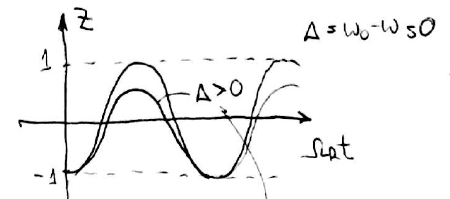
\includegraphics[width=0.6\linewidth]{fig/L5/invers_population}
	\caption{Inverse population of two level system for resonant and non-resonant excitation}
	\label{fig:inverspopulation}
\end{figure}
Let the incident field be $\vec{E} = \vec{E}_0 \cos \left( \omega t + \varphi \right)$. Induced dipole moment is $\vec{d}_{ab} = \bra{a} e \vec{r} \ket{b} \in \mathbb{C}$, so $\left| \bm{\Omega} \right| = \Omega_R = \frac{\vec{E}_0 \cdot \vec{d}_{ab}}{\hbar}$. 

\textit{Remark:} dissipation terms with parameter $\Gamma$ can be easily added to \eqref{eq:tmp_system} (\textcolor{red}{see Scully, find where!}).

\begin{otherlanguage}{russian}
	\begin{hw}[Можно здесь добавить домашку про построение сферы Блоха с затуханием и, например, указать сразу пример системы с $\Gamma \neq 0$.]
		\textcolor{red}{бла бла бла}
	\end{hw}
\end{otherlanguage}


For better understanding we consider a few typical cases: 
\begin{enumerate}
	\item Resonant and non-resonant excitation without dissipation ($\Gamma = 0$). See fig. \ref{fig:bloch1}.
	\begin{figure}[h!]
		\centering
		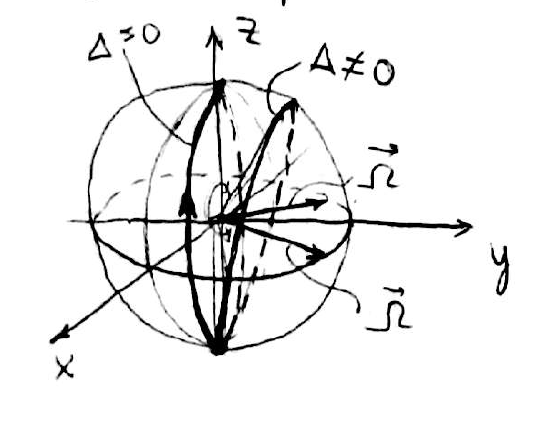
\includegraphics[width=0.7\linewidth]{fig/L5/bloch1}
		\caption{Resonant and non-resonant excitation}
		\label{fig:bloch1}
	\end{figure}
	\item $\Gamma \neq 0$, $\Tr \hat{\rho} = 1$ --- elastic dissipations. See fig. \ref{fig:gammanenol1}.
	\begin{figure}[h!]
		\centering
		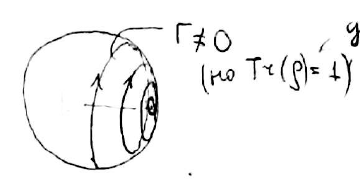
\includegraphics[width=0.6\linewidth]{fig/L5/gamma_ne_nol_1}
		\caption{$\Gamma \neq 0$, $\Tr \hat{\rho} = 1$}
		\label{fig:gammanenol1}
	\end{figure}
	\item $\Gamma \neq 0$, $\Tr \hat{\rho} \neq 1$ --- non-elastic dissipations. See fig. \ref{fig:gammanenol}.
	\begin{figure}[h!]
		\centering
		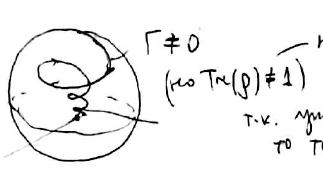
\includegraphics[width=0.6\linewidth]{fig/L5/gamma_ne_nol}
		\caption{$\Gamma \neq 0$, $\Tr \hat{\rho} = 1$. Block sphere ejection}
		\label{fig:gammanenol}
	\end{figure}
	
	
\end{enumerate}

	
	\section{Atom--field interaction. Quantum approach}

\subsection{Jaynes–Cummings model (RWA)}

\begin{figure}[h!]
	\centering
	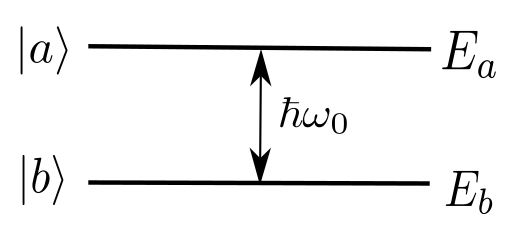
\includegraphics[width=0.3\linewidth]{fig/L6/2lvl}
	\caption{Two--level system}
	\label{fig:22lvl}
\end{figure}

Hamiltonian of system "quantum atom" $+$ "quantum field":
\begin{equation}
	\hat{\mathscr{H}} = \hat{\mathscr{H}}_A + \hat{\mathscr{H}}_F + \hat{\mathscr{H}}_{int}.
\end{equation}
where $\hat{\mathscr{H}}_A$ describes only \textit{atom}, $\hat{\mathscr{H}}_F$ describes only \textit{\textbf{quantized} field} and $\hat{\mathscr{H}}_{int}$ --- interaction part. Explicit expressions are:
\begin{eqnarray}
	\hat{\mathscr{H}}_A &=& E_a \ket{a} \bra{a} + E_b \ket{b} \bra{b}, \\
	\hat{\mathscr{H}}_F &=& \sum_{\vec{k}} \hbar \omega_{\vec{k}} \left( \hat{n}_{\vec{k}} + \frac{1}{2} \right), \qquad \hat{n}_{\vec{k}} = \hat{a}^{\dagger}_{\vec{k}} \hat{a}_{\vec{k}}, \\
	\hat{\mathscr{H}}_{\text{int}} &=& -e \vec{r} \cdot \hat{\vec{E}},
\end{eqnarray}
where field operator is given by
\begin{equation}
	\hat{\vec{E}} = \sum_{\kv} \varepsilon_{\kv} \left( \hat{a}_{\kv} \vec{e}_{\kv} e^{i \kv \vec{r}} + \hat{a}^{\dagger}_{\kv} \vec{e}^*_{\kv} e^{-i \kv \vec{r}} \right),
\end{equation}
where $\vec{e}_{\kv}$ is polarization vector. For simplicity we consider case $\vec{k} = 0$ and $\vec{e}_{\kv} \in \mathbb{R}$ so we have
\begin{equation}
	\hat{\vec{E}} = \sum_{\vec{k}} \vec{e}_{\vec{k}} \varepsilon_{\kv} \left( \hat{a}^{\dagger}_{\kv} + \hat{a}_{\kv} \right).
\end{equation}
Now let us rewrite dipole moment:
\begin{equation}
	e \vec{r} = \hat{\mathbb{1}} \cdot e \vec{r} \cdot \hat{\mathbb{1}} = \sum_{i,j = a,b} \ket{i} \underbrace{\bra{i}  e \vec{r} \ket{j}}_{\vec{d}_{ij}} \bra{j} = \sum_{ij} \vec{d}_{ij} \underbrace{\ket{i} \bra{j}}_{\hat{\sigma}_{ij}} = \sum_{ij} \vec{d}_{ij} \hat{\sigma}_{ij}.
\end{equation}
Here we denoted:
\begin{equation}
	\vec{d}_{ij} \myeq \bra{i}  e \vec{r} \ket{j}, \qquad \hat{\sigma}_{ij} \myeq  \ket{i} \bra{j}.
\end{equation}
Then
\begin{equation}
	\hat{\mathscr{H}}_{\text{int}} = - \sum_{ij} \sum_{\kv} \left(\vec{d}_{ij} \cdot \vec{e}_{\kv}\right) \sigma_{ij} \varepsilon_{\kv} \left( \hat{a}^{\dagger}_{\kv} + \hat{a}_{\kv} \right).
\end{equation}
Introduce a new notation:
\begin{equation}
	\boxed{	g_{ij}^{\kv} \myeq - \frac{ \varepsilon_{\kv} \left(\vec{d}_{ij} \cdot  \vec{e}_{\kv}\right)}{\hbar}.}
\end{equation}
This is a similarity to Rabi frequency but for one mode of field. To simplify computations let $g^{\kv}_{ij} \in \mathbb{R}$. So our Mr. Hamiltonian
\begin{equation}
	\hat{\mathscr{H}} = E_a \hat{\sigma}_{aa} + E_b \hat{\sigma}_{bb} + \sum_{\vec{k}} \hbar \omega_{\kv} \left( \hat{a}^{\dagger}_{\kv} \hat{a}_{\kv} + \half \right) + \sum_{ij} \sum_{\kv} \hbar g_{ij}^{\kv} \hat{\sigma}_{ij} \left( \hat{a}^{\dagger}_{\kv} +  \hat{a}_{\kv} \right).
\end{equation}
\begin{figure}
	\centering
	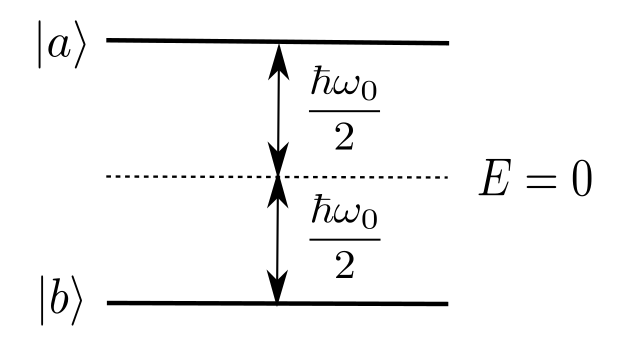
\includegraphics[width=0.4\linewidth]{fig/L6/E00000}
	\caption{A free choice of initial energy level}
	\label{fig:e00000}
\end{figure}
Let us put a starting energy point right in between $E_a$ and $E_b$ (fig.\ref{fig:e00000}). If we do so then
\begin{equation}
	E_a \hat{\sigma}_{aa} + E_b \hat{\sigma}_{bb} = \half \hbar \omega_0 \left( \hat{\sigma}_{aa} - \hat{\sigma}_{bb} \right) + \half \left( E_a + E_b \right)\underbrace{\left( \hat{\sigma}_{aa} + \hat{\sigma}_{bb} \right)}_{\hookrightarrow = \hat{\mathbb{1}}}.
\end{equation}
After that we make a transition to the new Hamiltonian by this energy shift
\begin{equation}
	\hat{\mathscr{H}} - \half \left( E_a + E_b \right) \quad \to \quad \hat{\mathscr{H}}.
\end{equation}

It is convenient to make new denotions:
\begin{eqnarray}
	\hat{\sigma}_{z} &\myeq& \hat{\sigma}_{bb} - \hat{\sigma}_{aa}, \\
	\hat{\sigma}_{+} &\myeq& \hat{\sigma}_{ab} = \ket{a} \bra{b}, \\
	\hat{\sigma}_{-} &\myeq& \hat{\sigma}_{ba} = \ket{b} \bra{a},
\end{eqnarray}
where
\begin{equation}
	\ket{b} = \begin{pmatrix}
		1 \\ 0
	\end{pmatrix}, \qquad
	\ket{a} = \begin{pmatrix}
	0 \\ 1
	\end{pmatrix},
\end{equation}
so reader may easily construct matrices for $\hat{\sigma}_{z}$, $\hat{\sigma}_{+}$ and $\hat{\sigma}_{-}$:
\begin{equation}
	\hat{\sigma}_z = \begin{pmatrix}
	1 & 0 \\ 0 & -1
	\end{pmatrix}, \qquad
	\hat{\sigma}_+ = \begin{pmatrix}
	0 & 0 \\ 1 & 0
	\end{pmatrix}, \qquad
	\hat{\sigma}_- = \begin{pmatrix}
	0 & 1 \\ 0 & 0
	\end{pmatrix}.
\end{equation}
To answer how act new operators $\hat{\sigma}_{+}$ and $\hat{\sigma}_{-}$ consider the following:
\begin{eqnarray}
	\hat{\sigma}_{+} \ket{b} = \ket{a} \braket{b}{b} = \ket{a}, \\
	\hat{\sigma}_{-} \ket{a} = \ket{b} \braket{a}{a} = \ket{b}.
\end{eqnarray}
The operator $\hat{\sigma}_{+}$ takes the system from lower state to upper states vice versa.

Usually $\vec{d}_{aa} = \vec{d}_{bb} = 0$, so
\begin{equation}
	g^{\kv}_{aa} = 0, \qquad g^{\kv}_{bb} = 0,
\end{equation}
\begin{equation}
	g^{\kv}_{ab} = g^{\kv}_{ba} \myeq g^{\kv}.
\end{equation}
After that Hamiltonian may be written as
\begin{equation}
	\hat{\mathscr{H}} = \underbrace{\sum_{\kv} \hbar \omega_{\kv} \left( \hat{a}_{\kv}^{\dagger}\hat{a}_{\kv} + \half \right)}_{\text{field}} + \underbrace{\frac{\hbar \omega_0}{2} \hat{\sigma}_z}_{\text{atom}} + \underbrace{\hbar \sum_{\kv} g^{\kv} \left( \hat{\sigma}_+ + \hat{\sigma}_- \right) \left( \hat{a}^{\dagger}_{\kv} + \hat{a}_{\kv} \right)}_{\text{interaction}}.
\end{equation}

Algebra of new operators:
\begin{eqnarray}
	\left[ \hat{\sigma}_-, \hat{\sigma}_+ \right] &=& - \hat{\sigma}_z, \\
	\left[ \hat{\sigma}_-, \hat{\sigma}_z \right] &=& 2\hat{\sigma}_-, \\
	\left[ \hat{\sigma}_+, \hat{\sigma}_z \right] &=& -2 \hat{\sigma}_+, \\
	\left\{ \hat{\sigma}_+, \hat{\sigma}_- \right\} &=& \hat{\mathbb{1}}.
\end{eqnarray}
Last property is rooted in fact that electrons are fermions. $\hat{\sigma}_+$ and $\hat{\sigma}_-$ are creation and annihilation operators for electron in atom. Lets consider the physical meaning of the interactive terms:
\begin{equation}
	\left( \hat{\sigma}_+ + \hat{\sigma}_- \right) \left( \hat{a}^{\dagger}_{\kv} + \hat{a}_{\kv} \right) = \underbrace{\hat{\sigma}_+ \hat{a}}_{\text{(I)}} + \overbrace{\underbrace{\cancel{\hat{\sigma}_+ \hat{a}^{\dagger}}}_{\text{(II)}} + \underbrace{\cancel{\hat{\sigma}_- \hat{a}}}_{\text{(III)}}}^{\text{unphysical}} + \underbrace{\hat{\sigma}_- \hat{a}^{\dagger}}_{\text{(IV)}},
\end{equation}
where (I) --- photon annihilation and electron excitation, (II) --- photon creation and electron excitation, (III) --- photon annihilation and electron relaxation, (IV) --- photon creation and electron relaxation. Terms  $\hat{\sigma}_+\hat{a}^{\dagger} + \hat{\sigma}_-\hat{a}$ are unphysical, so \textit{may be omitted}. In fact this is the RWA. After such assumption we have:
\begin{equation}
	\boxed{\hat{\mathscr{H}} = \sum_{\kv} \hbar \omega_{\kv} \left( \hat{a}_{\kv}^{\dagger}\hat{a}_{\kv} + \half \right) + \frac{\hbar \omega_0}{2} \hat{\sigma}_z + \sum_{\kv} \hbar g^{\kv} \left( \hat{\sigma}_+\hat{a}_{\kv} + \hat{a}^{\dagger}_{\kv} \hat{\sigma}_- \right).}
\end{equation}

For simplicity let us consider one mode field
\begin{equation}
	\hat{\mathscr{H}} = \underbrace{\hbar \omega \left( \hat{a}^{\dagger}\hat{a} + \half \right) + \frac{\hbar \omega_0}{2} \hat{\sigma}_z}_{\hat{\mathscr{H}}_0} + \underbrace{\hbar g \left( \hat{\sigma}_+\hat{a} + \hat{a}^{\dagger} \hat{\sigma}_- \right)}_{\hat{V}}.
	\label{eq:hamillll}
\end{equation}
Now we pass into the representation of interaction
\begin{equation}
	\hat{\mathscr{H}}_V = e^{\frac{i}{\hbar} \hat{\mathscr{H}}_0 t} \hat{V} e^{-\frac{i}{\hbar} \hat{\mathscr{H}}_0 t}.
\end{equation}
\begin{enumerate}
	\item[\textit{Remark}:] \textit{The interaction representation means the following.
	After unitary transformation }
	\begin{equation*}
	\ket{\widetilde{\psi}} = e^{\frac{i}{\hbar} \hat{\mathscr{H}}_0 t} \ket{\psi}, \qquad \hat{\mathscr{H}} \to \hat{\mathscr{H}}_V
	\end{equation*}
	\textit{we obtain new effective Schrödinger equation}
	\begin{equation*}
	i \hbar \dot{\ket{\psi}} = \hat{\mathscr{H}} \ket{\psi} \quad \to \quad i \hbar \dot{\ket{\widetilde{\psi}}} = \hat{\mathscr{H}}_V \ket{\widetilde{\psi}}.
	\end{equation*}
\end{enumerate}
Let us begin. We need to consider
\begin{equation}
	e^{i \frac{\omega_0}{2} \hat{\sigma}_z t} e^{i \omega \hat{a}^{\dagger} \hat{a} t} \hat{V} e^{-i \omega \hat{a}^{\dagger} \hat{a} t} e^{-i \frac{\omega_0}{2} \hat{\sigma}_z t}.
\end{equation}
Different terms will appear:
\begin{eqnarray}
	e^{i \omega \hat{a}^{\dagger} \hat{a} t} \hat{a} e^{-i \omega \hat{a}^{\dagger} \hat{a} t} &=& \hat{a} e^{- i\omega t}, \\
	e^{i \omega \hat{a}^{\dagger} \hat{a} t} \hat{a}^{\dagger} e^{-i \omega \hat{a}^{\dagger} \hat{a} t} &=& \hat{a}^{\dagger} e^{i \omega t}, \\
	e^{i \frac{\omega_0}{2} \hat{\sigma}_z t} \hat{\sigma}_+ e^{-i \frac{\omega_0}{2} \hat{\sigma}_z t} &=& \hat{\sigma}_+ e^{i \omega_0 t}, \\
	e^{i \frac{\omega_0}{2} \hat{\sigma}_z t} \hat{\sigma}_- e^{-i \frac{\omega_0}{2} \hat{\sigma}_z t} &=& \hat{\sigma}_- e^{-i \omega_0 t}.
\end{eqnarray}
So
\begin{equation}
	\hat{\mathscr{H}}_V = \hbar g \left( \hat{a}^{\dagger} \hat{\sigma}_- e^{-i (\omega_0 - \omega)t} + \hat{\sigma}_+ \hat{a} e^{i (\omega_0 - \omega)t} \right).
\end{equation}
As a matter of convenience we introduce $\Delta \myeq \omega_0 - \omega$. An effective Schrödinger equation now may be written as
\begin{equation}
	\quad i \hbar \parder{}{t}\ket{\widetilde{\psi}} = \hat{\mathscr{H}}_V \ket{\widetilde{\psi}}.
\end{equation}
After that we expand wave function in series
\begin{equation}
	\ket{\widetilde{\psi}} = \sum_{n} C_{a,n}(t) \ket{n} \ket{a} + \sum_{n} C_{b,n}(t) \ket{n} \ket{b},
\end{equation}
where $C_{a,n}(t)$ --- a probability of finding an electron in $\ket{a}$ and a photon in $\ket{n}$ at time $t$. To bring into focus results we omit all the computations and present only the solution:
\begin{equation}
	\begin{cases}
		i \hbar \dot{C}_{a,n}(t) = \hbar g \sqrt{n+1} C_{b,n+1}(t) e^{i \Delta t}, \\
		i \hbar \dot{C}_{b,n+1}(t) = \hbar g \sqrt{n+1} C_{a,n}(t) e^{-i \Delta t}.
	\end{cases}
	\label{eq:228_botat_my_ne_brosim}
\end{equation}

\begin{figure}
	\centering
	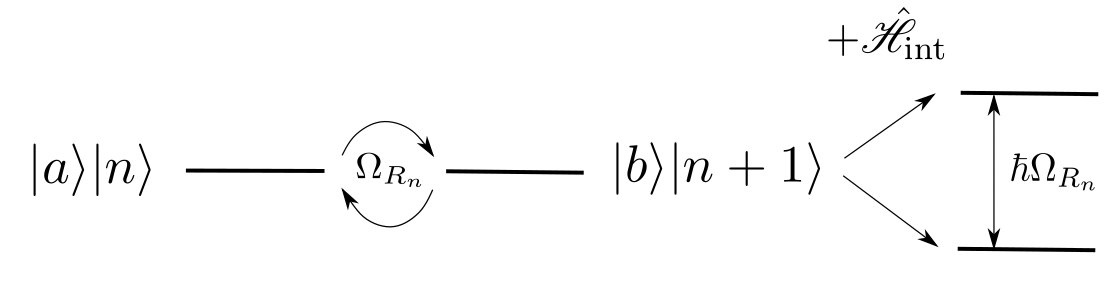
\includegraphics[width=0.8\linewidth]{fig/L6/E_split}
	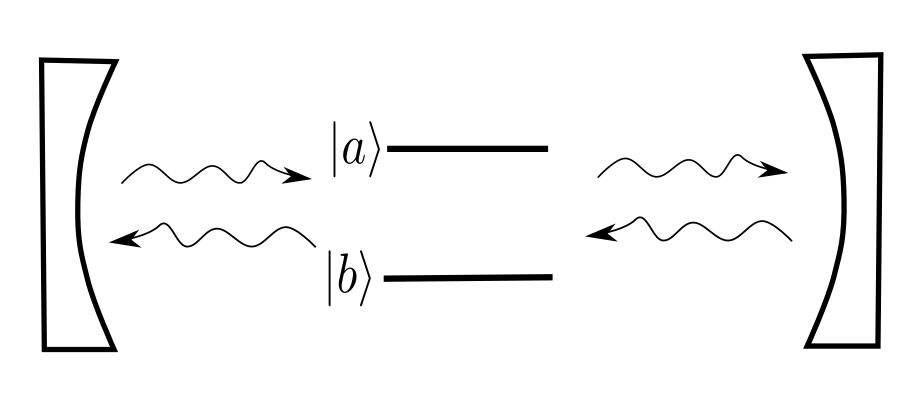
\includegraphics[width=0.5\linewidth]{fig/L6/osc_in_cavity}
	\caption{Oscillations in a cavity}
	\label{fig:228}
\end{figure}


For simplicity let us consider a resonant excitation, it means we need to put $\Delta  =0$ in \eqref{eq:228_botat_my_ne_brosim}. After we have
\begin{equation}
	\begin{cases}
		\dot{C}_{a,n}(t) = -i g \sqrt{n+1} C_{b,n+1}(t) \\
		\dot{C}_{b,n+1}(t) = -i g \sqrt{n+1} C_{a,n}(t)
	\end{cases} \qquad \to \qquad
	\ddot{C}_{a,n} (t) + \underbrace{g^2(n+1)}_{\Omega_{R_n}^2} C_{a,n}(t) = 0.
\end{equation}
Easy to notice, we obtained osculations with angular frequency
\begin{equation}
	\boxed{\Omega_{R_n} = g \sqrt{n+1}.}
\end{equation}
A physical interpretation of such oscillations is shown in fig. \ref{fig:228}.

\begin{testexample}[Vacuum Rabi oscillations.]
	If we put $n=0$ we get $\Omega_{R_0} = g \neq 0$. We have a vacuum interaction: no field, interaction exists!
	%\textcolor{red}{(UNCOMMENT THIS LATER! (see source))}
\end{testexample}



\begin{hw}[Deadline: 29th of December]
	\addcontentsline{toc}{subsubsection}{Homework}

	\begin{enumerate}
		\item (6 pts) (See problem 6.2 from Scully). One of the common models of light-atom interaction in a cavity can be described by the Hamiltonian :
		$$
		H=\hbar\omega_{0}\sigma_{z}+ \hbar \omega a^{+}a+\hbar g(\sqrt{a^{+}a}a^{+}\sigma_{-}+\sigma_{+}a\sqrt{a^{+}a}),
		$$
		where interaction depends on the intensity. Compute the inverse population at the timescale of Rabi oscillations, considering  initial state of photons as coherent.
	\end{enumerate}
\end{hw}


\subsection{Collapse and revival}

Another important quantity is the inversion $W(t)$ which is related to the probabilty amplitudes $C_{a,n}(t)$ and $C_{b,n}(t)$ by the expression
\begin{equation}
	W(t) = \sum_{n} \left( \left| C_{a,n}(t) \right|^2 - \left| C_{b,n}(t) \right|^2 \right).
\end{equation}
In fig. \ref{fig:candr} $W(t)$ is plotted as a function of normalized time $g t$ for an initial coherent state. The behavior of $W(t)$ is quite different from the corresponding curve (fig. \ref{fig:rabiosc}) in the semiclassical theory. In the present case the envelope of the sinusoidal Rabi oscillations '\textit{collapses}' to zero. However as time increases we encounter a '\textit{revival}' of the collapsed inversion. This behavior of collapse and revival of inversion is repeated with increasing time, with the amplitude of Rabi osculations decreasing and the time duration in which revival takes place increasing and ultimately overlapping with the earlier revival.

\begin{figure}
	\centering
	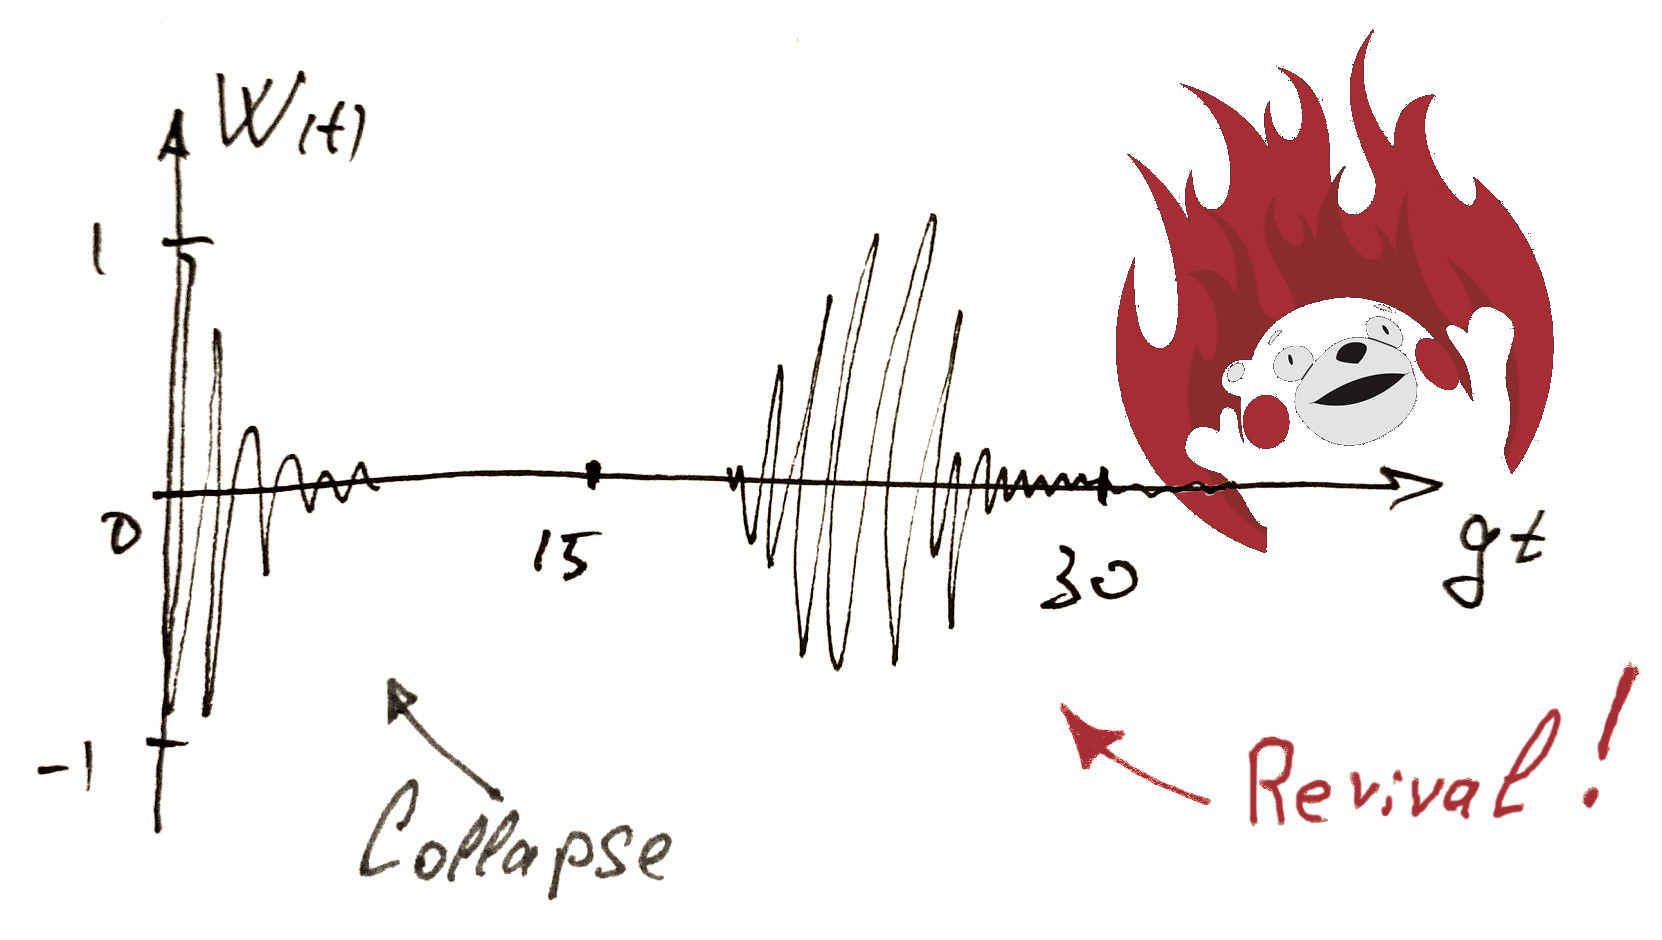
\includegraphics[width=0.7\linewidth]{fig/L6/c_and_r.jpg}
	\caption{Time evolution of the population inversion $W(t)$ for an initially coherent state.}
	\label{fig:candr}
\end{figure}


\subsection{Energy spectrum. Dispersion relation}

Let us find eigenstates of $\hat{\mathscr{H}}$ which is given by \eqref{eq:hamillll}. Here, for convenience, the vacuum field energy is set to $0$, so
\begin{equation}
	\hat{\mathscr{H}} = \underbrace{\hbar \omega  \hat{n} + \frac{\hbar \omega_0}{2} \hat{\sigma}_z}_{\hat{\mathscr{H}}_0} + \underbrace{\hbar g \left( \hat{\sigma}_+\hat{a} + \hat{a}^{\dagger} \hat{\sigma}_- \right)}_{\hat{\mathscr{H}}_{\text{int}}}.
\end{equation}

The equation for eigenvalues is
\begin{equation}
\hat{\mathscr{H}} \ket{\psi} = E \ket{\psi}.
\label{eq:eigen}
\end{equation}
Next terms will appear:
\begin{eqnarray}
	\hat{\mathscr{H}}_0 \ket{a} \ket{n} &=& \left( \frac{\hbar \omega_0}{2} + \hbar \omega n \right) \ket{a} \ket{n}, \\
	\hat{\mathscr{H}}_0 \ket{b} \ket{n+1} &=& \left( -\frac{\hbar \omega_0}{2} + \hbar \omega n \right) \ket{b} \ket{n+1}, \\
	\hat{\mathscr{H}}_{\text{int}} \ket{a} \ket{n} &=& \hbar g \sqrt{n+1} \ket{b} \ket{n+1}, \\
	\hat{\mathscr{H}}_{\text{int}} \ket{b} \ket{n+1} &=& \hbar g \sqrt{n+1} \ket{a} \ket{n}.
\end{eqnarray}
Important to notice that number of quantas is concerned, if we take  basis $\ket{a} \ket{n}$ and $\ket{b} \ket{n+1}$. After acting $\hat{\mathscr{H}}_{\text{int}}$ we stay in the same subspace with the same basis. Consequently, eigenfunctions may be written as
\begin{equation}
	\ket{\psi} = \ket{\varphi_1} \cdot \ket{\varphi_2} \cdot ... \cdot \ket{\varphi_n} \cdot ...
\end{equation}
Each of $\ket{\varphi_n}$ acts on its own subspace and does not affect the others:
\begin{equation}
	\ket{\varphi_n} = c_n \ket{a} \ket{n} + c_{2n} \ket{b} \ket{n+1}.
\end{equation}
It leads to a very imports consequence --- $\hat{\mathscr{H}}$ is \textit{block-diagonal matrix}:
\begin{equation}
	\hat{\mathscr{H}} =
	\begin{pmatrix}
		\hat{\mathcal{H}}_1 & 0 & 0 & \dots & 0 & \dots \\
		0& \hat{\mathcal{H}}_2 &0 & \dots &0 & \dots\\
		\vdots & \dots  & \ddots & \dots & \vdots & \dots \\
		0 & \dots & 0& \hat{\mathcal{H}}_n & 0 & \dots \\
		\vdots & \vdots & \vdots & \ddots & \ddots & \ddots
	\end{pmatrix}.
\end{equation}
Where each of $\hat{\mathcal{H}}_n$ is a $2\times2$ matrix.

Looking for an energy spectrum \eqref{eq:eigen} is equivalent to the Hamiltonian diagonalization.
We simplified our problem and now we need only to diagonalize $2 \times 2$ matrices or in other words we need to solve
\begin{equation}
	\hat{\mathcal{H}}_n \ket{\varphi_n} = E_n \ket{\varphi_n}.
\end{equation}

In an explicit form we need to diagonalize
\begin{multline}
	\hat{\mathcal{H}}_n = \hat{\mathcal{H}}^0_{n} + \hat{\mathcal{H}}^{\text{int}}_n =
	\begin{pmatrix}
		\frac{\hbar \omega_0}{2} + \hbar \omega n & 0 \\
		0 & - \frac{\hbar \omega_0}{2} + \hbar \omega n
	\end{pmatrix} +
	\begin{pmatrix}
		0 & \hbar g \sqrt{n+1} \\
		\hbar g \sqrt{n+1} & 0
	\end{pmatrix} = \\ \\ =
	\hbar \omega \left( n+ \half \right) \hat{I}
	+ \frac{\hbar}{2} \begin{pmatrix}
		\Delta & 2g \sqrt{n+1} \\ \\
		2g \sqrt{n+1} & - \Delta
	\end{pmatrix},
\end{multline}
where $\Delta = \omega - \omega_0$ and $\hat{I} = \begin{pmatrix}
1 & 0 \\
0 & 1
\end{pmatrix}$ is an identity matrix. Human by nature is lazy, so we do. It means let us consider a simple case when $\Delta = 0$, so
\begin{equation}
	\det \left( \hat{\mathcal{H}}_n - E \hat{I} \right) = 0 \quad \to \quad \left( E - \hbar \omega (n + \half) \right) = \hbar^2 g^2 (n+1)
\end{equation}
or
\begin{equation}
	\begin{cases}
		E_1 = \hbar \omega \left( n + \half \right) + \hbar g \sqrt{n+1}, \\
		E_2 = \hbar \omega \left( n + \half \right) - \hbar g \sqrt{n+1}.
	\end{cases}
\end{equation}
\begin{figure}
	\centering
	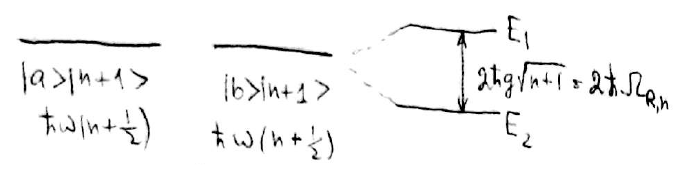
\includegraphics[width=0.7\linewidth]{fig/L6/leveeeelllls}
	\caption{Level splitting after acting $\hat{\mathcal{H}}_n$}
	\label{fig:leveeeelllls}
\end{figure}
This energy splitting is shown in fig. \ref{fig:leveeeelllls}. If we consider case $\Delta \neq 0$ then we will get
\begin{equation}
	\begin{cases}
	E_1 = \hbar \omega \left( n + \half \right) + \half \hbar R_n, \\
	E_2 = \hbar \omega \left( n + \half \right) - \half \hbar R_n,
	\end{cases}
	\label{eq:system57}
\end{equation}
where $R_n = \sqrt{\Delta^2 + 4g^2 (n+1)}$.
\begin{figure}
	\centering
	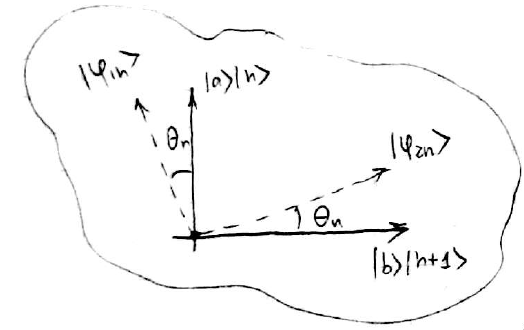
\includegraphics[width=0.65\linewidth]{fig/L6/rotation}
	\caption{Rotation in a subspace}
	\label{fig:rotation}
\end{figure}

Eigenstates may be written as a rotated $\ket{a,n}$ and $\ket{b,n+1}$ states
\begin{equation}
	\begin{cases}
		\ket{\varphi_{1n}} = \cos \vartheta_n \ket{a, n} + \sin \vartheta_n \ket{b ,n +1}, \\
		\ket{\varphi_{2n}} = -\sin \vartheta_n \ket{a, n} + \cos \vartheta_n \ket{b ,n +1},
	\end{cases}
\end{equation}
where $\cos \vartheta_n = \frac{2 g \sqrt{n+1}}{\sqrt{(R_n - \Delta)^2 + 4 g^2 (n+1)}}$. Just to make things clear, $\ket{a,n}$ and $\ket{b,n+1}$ are eigenfunctions of $\hat{\mathcal{H}}^0_{n}$, after 'turning on' an interaction we gain a plane rotation!


States $\ket{\varphi_{1n}}$ and $\ket{\varphi_{2n}}$ --- \textit{polariton states}. This is a mixed stated of light and medium.


For $\Delta = 0$ we have $\vartheta = \frac{\pi}{4}$. It means that
\begin{equation}
	\begin{cases}
		\ket{\varphi_{1n}} = \frac{1}{\sqrt{2}} \left(\ket{a, n} + \ket{b ,n +1}\right), \\
		\ket{\varphi_{2n}} = \frac{1}{\sqrt{2}}\left(-\ket{a, n} + \ket{b ,n +1}\right).
	\end{cases}
\end{equation}
Energy is given by \eqref{eq:system57}. If there is no interaction ($g = 0$) we have
\begin{equation}
	\begin{cases}
		E_{1n} = \hbar \omega \left( n + \half\right) + \frac{\hbar}{2} \Delta, \\
		E_{2n} = \hbar \omega \left( n + \half\right) - \frac{\hbar}{2} \Delta.
	\end{cases}
\end{equation}
Not let us make a graphical analysis. At first shall we put $n=0$ and $g=0$ (fig. \ref{fig:n0}). After that we 'turn on' interaction ($n=0$, $g \neq 0$) and we get fig. \ref{fig:n0gne0}. All necessary comments are given under the figures.

\begin{figure}
	\centering
	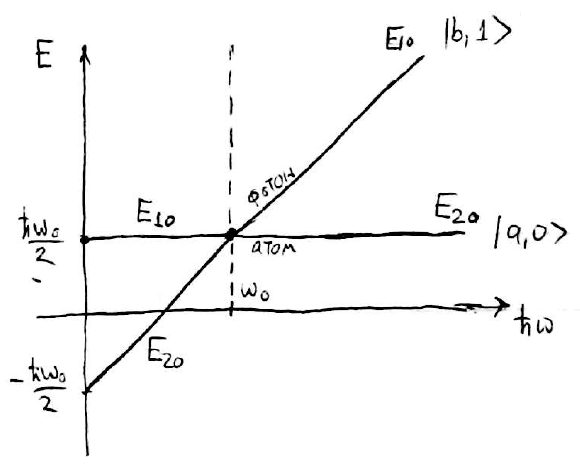
\includegraphics[width=0.5\linewidth]{fig/L6/n0}
	\caption{Case of $n=0$ and $g=0$. State $\ket{b,1}$ --- there is a photon with energy $\hbar \omega$, so $E = E(\omega)$ is linear. State $\ket{a,0}$ --- no photon in cavity, energy does not depend on $\hbar \omega$, there is an exciton}
	\label{fig:n0}
\end{figure}
\begin{figure}
	\centering
	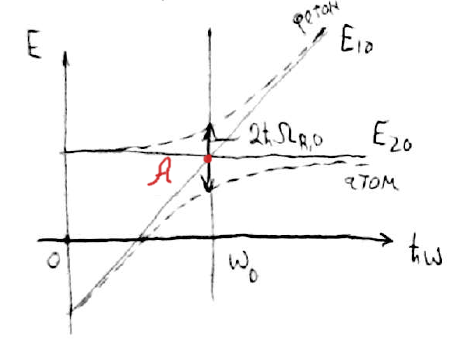
\includegraphics[width=0.5\linewidth]{fig/L6/n0_g_ne0}
	\caption{Case of $n=0$ and $g\neq0$. Line splitting is observed. At frequency $\omega_0$ there is no pure atom state nor photon state --- it is mixed state, polariton state}
	\label{fig:n0gne0}
\end{figure}

At point A on fig. \ref{fig:n0gne0} quantum of energy neither in atom nor in photon, it is equidistant from $E_{01}$ and $E_{02}$. This is a \textit{polariton state}!

In fact we described a so called Cummings ladder (fig. \ref{fig:lad}).
\begin{figure}
	\centering
	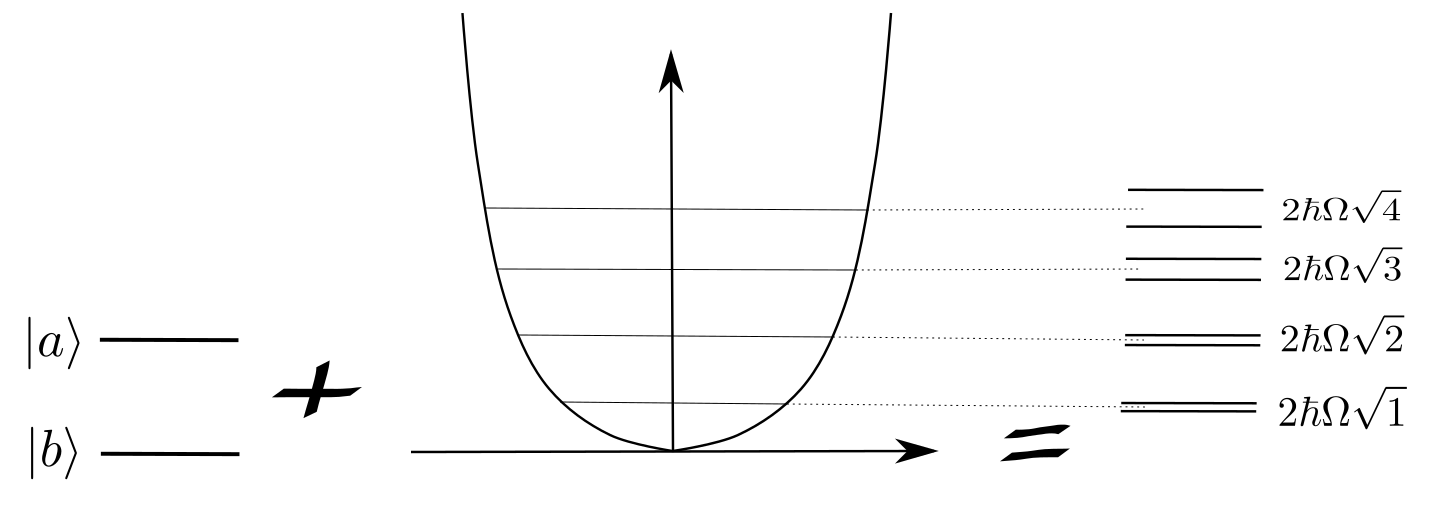
\includegraphics[width=0.6\linewidth]{fig/L6/lad}
	\caption{Cummings ladder. Energy splitting as a result of combining two quantum systems: atom and field}
	\label{fig:lad}
\end{figure}

	
	\section{Spontaneous relaxation. Weisskopf-Wigner theory}

We have shown that excited two-level atom can perform transitions from the upper state to the lower state and vice versa even \textit{without} external field. Intuitively clear that such process cannot last forever and experiments prove this idea. In our model before we did not have such relaxation process because we take in account only one mode of field (we neglected the continuum of modes in \eqref{eq:hamillll}). Fir a proper account of the atomic decay a continuum of modes, corresponding to a quantization cavity which is infinite in extent, needs to be included.

\begin{figure}[h!]
	\centering
	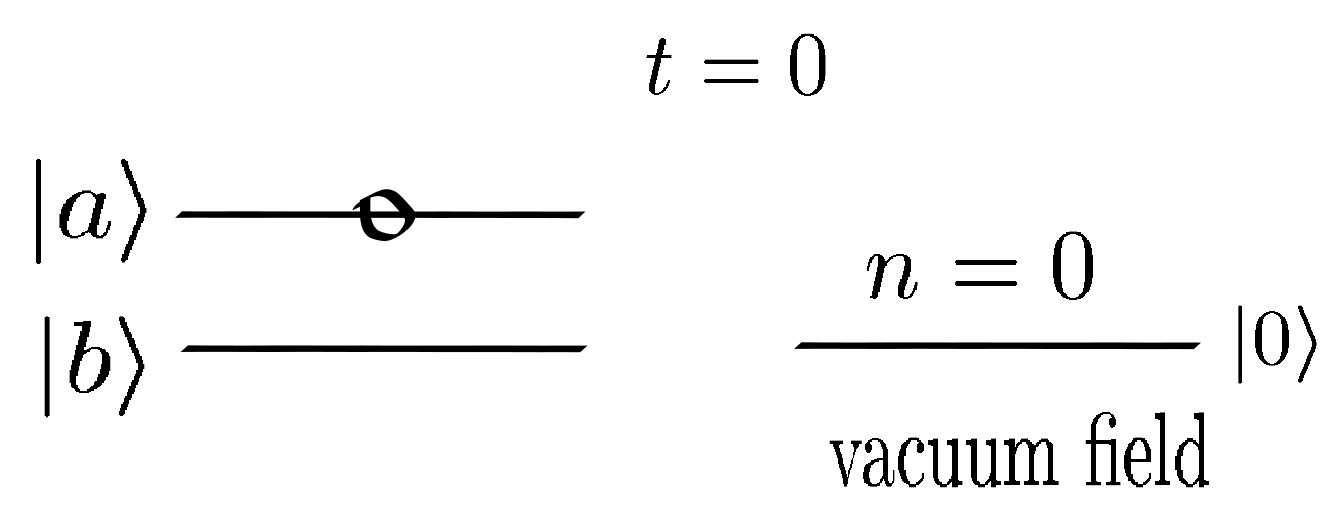
\includegraphics[width=0.5\linewidth]{fig/L7/1}
	\caption{Initial conditions}
	\label{fig:1}
\end{figure}

In other words we consider a two-level system in a huge box with linear dimension $L$ with quantized electromagnetic field inside.
The \textit{interaction picture} Hamiltonian, in the rotating-wave approximation, for this system is
\begin{equation}
	\hat{V}(t) = \hbar \sum_{\kv} \left[ g_{\kv}^* \hat{\sigma}_+ \hat{a}_{\kv} e^{i(\omega_0 - \omega_{\kv})t} + H.c. \right].
\end{equation}
We want to study the system dynamics. Wave functions
\begin{equation}
\ket{\psi(t)} = \sum_{n, \kv} \left( c_{a, n_{\kv}}(t) \ket{a} \ket{n_{\kv}} + c_{b, n_{\kv}}(t) \ket{b} \ket{n_{\kv}} \right),
\end{equation}
where $c_{a(b),n_{\kv}} \myeq c_{a(b), n_{\kv_1}, n_{\kv_2}, \dots}$ and $\ket{n_{\kv}} \myeq \ket{n_{\kv_1}} \ket{n_{\kv_2}} \cdot \dots$. We assume that at time $t=0$ the atom is in the excited state $\ket{a}$ and the field modes are in the vacuum state $\ket{0}$. The state vector is therefore: 
\begin{equation}
	\ket{\psi(t)} = c_{a,0}(t) \ket{a}\ket{0} + \sum_{\kv} c_{b, \kv}(t) \ket{b}\ket{1_{\kv}}, 
\end{equation}
which satisfies the interaction picture Schroedinger equation 
\begin{equation}
i \hbar \ket{\dot{\psi}(t)} = \hat{V}(t) \ket{\psi(t)}
\end{equation}
with initial conditions
\begin{equation}
	c_{a,0}(0) = 1, \qquad c_{b,\kv}(0) = 0.
\end{equation}

From the Schroedinger equation we get the equations of motion for the probability amplitudes:
\begin{subnumcases}{}
	\dot{c}_{a,0} (t) = -i \sum_{\kv} g_{\kv}^* e^{i \Delta_{\kv}t} c_{b,1_{\kv}}(t), \label{eq:7.6a} \\
	\dot{c}_{b,1_{\kv}} (t) = -i g_{\kv} e^{-i\Delta_{\kv}t} c_{a,0}(t), \label{eq:7.6b}
\end{subnumcases}
where $\Delta_{\kv} \myeq  \omega_0 - \omega_{\kv}$. To solve this system we, at first, $\int \eqref{eq:7.6b} dt$:
\begin{equation}
	c_{b,1_{\kv}} (t) = -i g_{\kv} \int \limits_{0}^{t} d \tau e^{-i \Delta_{\kv} \tau} c_{a,0}(\tau).
	\label{eq:tmpppppppp}
\end{equation}
After that we substitute \eqref{eq:tmpppppppp} to \eqref{eq:7.6a} and get the differential-integral equation
\begin{equation}
	\dot{c}_{a,0} (t) = - \sum_{\kv} \left| g_{\kv} \right|^2  \int \limits_0^t d \tau e^{-i \Delta_{\kv} (\tau - t)} c_{a,0}(\tau).
	\label{eq:77777}
\end{equation}
This is still an exact equation. Next shall we make some approximations.

Assuming that the modes of the field are closely spaced in frequency, we can
\begin{equation}
	\sum_{\kv} \qquad \overset{L\to \infty}{\longrightarrow} \qquad 2 \cdot V \int \frac{d^3 k}{(2 \pi)^3}
\end{equation}
where factor $2$ is from averaging over polarization and $\int d^3k = \int_{0}^{\infty} k^2 dk \int_{0}^{2 \pi} d\varphi  \int_{0}^{\pi} \sin \vartheta d \vartheta$ in spherical coordinate system. We remind that $g_{\kv} = - (\vec{d} \cdot \bm{\varepsilon}_{\kv}) / \hbar$ --- coupling constant between the atom and $\kv$-mode. System has a preferred direction: $\vec{d}$. Shall we write it explicitly
\begin{equation}
	g_{\kv} = - \frac{d \varepsilon_{\kv}}{\hbar} \cos \vartheta.
\end{equation}
This allows us easily integrate over $\vartheta$ and $\varphi$:
\begin{equation}
	\int \limits_{0}^{2 \pi} \int \limits_{0}^{\pi} \left| g_{\kv} \right|^2 \sin \vartheta d \varphi d \vartheta = \frac{\left(|\vec{d}| \varepsilon_{\kv}\right)^2}{\hbar^2} \cdot 2 \pi \int \limits_{0}^{\pi} d \vartheta \cos^2 \vartheta \sin \vartheta =  \frac{\left(|\vec{d}| \varepsilon_{\kv}\right)^2}{\hbar^2} \cdot \frac{4 \pi}{3}.
\end{equation}
It means that \eqref{eq:77777} becomes
\begin{equation}
	\dot{c}_{a,0} (t) = - \frac{2 V}{(2\pi \hbar)^3} \cdot \frac{4 \pi}{3} |\vec{d}|^2 \int \limits_{0}^{\infty} dk \int \limits_{0}^{t} d \tau k^2 \varepsilon_{\kv}^2 e^{-i \Delta_{\kv} (\tau - t)} c_{a,0}(\tau).
\end{equation}
Now shall we rewrite the $\int dk$ part using dispersion law $k = \omega_{\kv}/c$ and reminding that $\varepsilon_{\kv}^2 = \frac{\hbar \omega_{\kv}}{2 \varepsilon_0 V}$ (it comes from the expansion of electric field in ladder operators):
\begin{equation}
	\int \limits_{0}^{\infty} dk k^2 \frac{\hbar \omega_{\kv}}{2 \varepsilon_0 V} e^{-i \Delta_{\kv} (\tau - t)} = \frac{\hbar}{2 c^3 \varepsilon_0 V} \int \limits_0^{\infty} d \omega_{\kv} \omega_{\kv}^3 e^{-i (\omega_0 - \omega_{\kv})(\tau - t)},
\end{equation}
so
\begin{equation}
	\dot{c}_{a,0} (t) = - \frac{2 V}{(2\pi \hbar)^3} \cdot \frac{4 \pi}{3} |\vec{d}|^2 \cdot \frac{\hbar}{2 c^3 \varepsilon_0 V} \int \limits_{0}^{\infty} d \omega_{\kv} \int \limits_{0}^{t} d \tau \omega_{\kv}^3 e^{-i (\omega_0 - \omega_{\kv})(\tau - t)} c_{a,0}(\tau).
\end{equation}
In the emission spectrum, the intensity of light associated with the emitted radiation is going to be centered about the atomic transition frequency $\omega_0$. The quantity $\omega_{\kv}^3$ varies little around $\omega_{\kv} = \omega_0$ for which the time integral is not negligible. 
\begin{otherlanguage}{russian}	
\textcolor{red}{Что-то здесь мутный переход, мне не совсем понятно всё. Кстати, график подынтегрального выражения, что у Вас в конспекте в этом месте неверный, так не получится, если построить.}
\end{otherlanguage}
Therefore here we can use the \textit{stationary-phase method}:
\begin{equation}
	\int \limits_{0}^{\infty} d \omega_{\kv}  \omega_{\kv}^3 e^{-i (\omega_0 - \omega_{\kv})(\tau - t)} \quad \to \quad \omega_{0}^3 \int \limits_{-\infty}^{\infty} d \omega_{\kv} e^{-i (\omega_0 - \omega_{\kv})(\tau - t)} = \omega_{0}^3 \cdot 2 \pi \delta(\tau - t).
\end{equation}
Now integral over $d \tau$ is easy to take $\int_0^t d \tau \delta(\tau - t) c_{a,0}(\tau) = \frac{1}{2} c_{a,0}(t)$ and we finally obtain
\begin{equation}
	\dot{c}_{a,0} (t) = - \frac{\gamma}{2} c_{a,0} (t), \qquad \to \qquad c_{a,0}(t) = \exp \left[- \frac{\gamma}{2} t \right],
\end{equation}
where the \textit{decay constant}
\begin{equation}
	\gamma \myeq \frac{\omega_{0}^3 |\vec{d}|^2}{3 \pi \hbar c^3 \varepsilon_0}.
\end{equation}
If we consider a medium which effectively change the wave vector  $k \to nk$ with refractive index $n$ then we get
\begin{equation}
	\gamma = \frac{\omega_{0}^3 |\vec{d}|^2 n}{3 \pi \hbar c^3 \varepsilon_0}.
\end{equation}
\begin{figure}
	\centering
	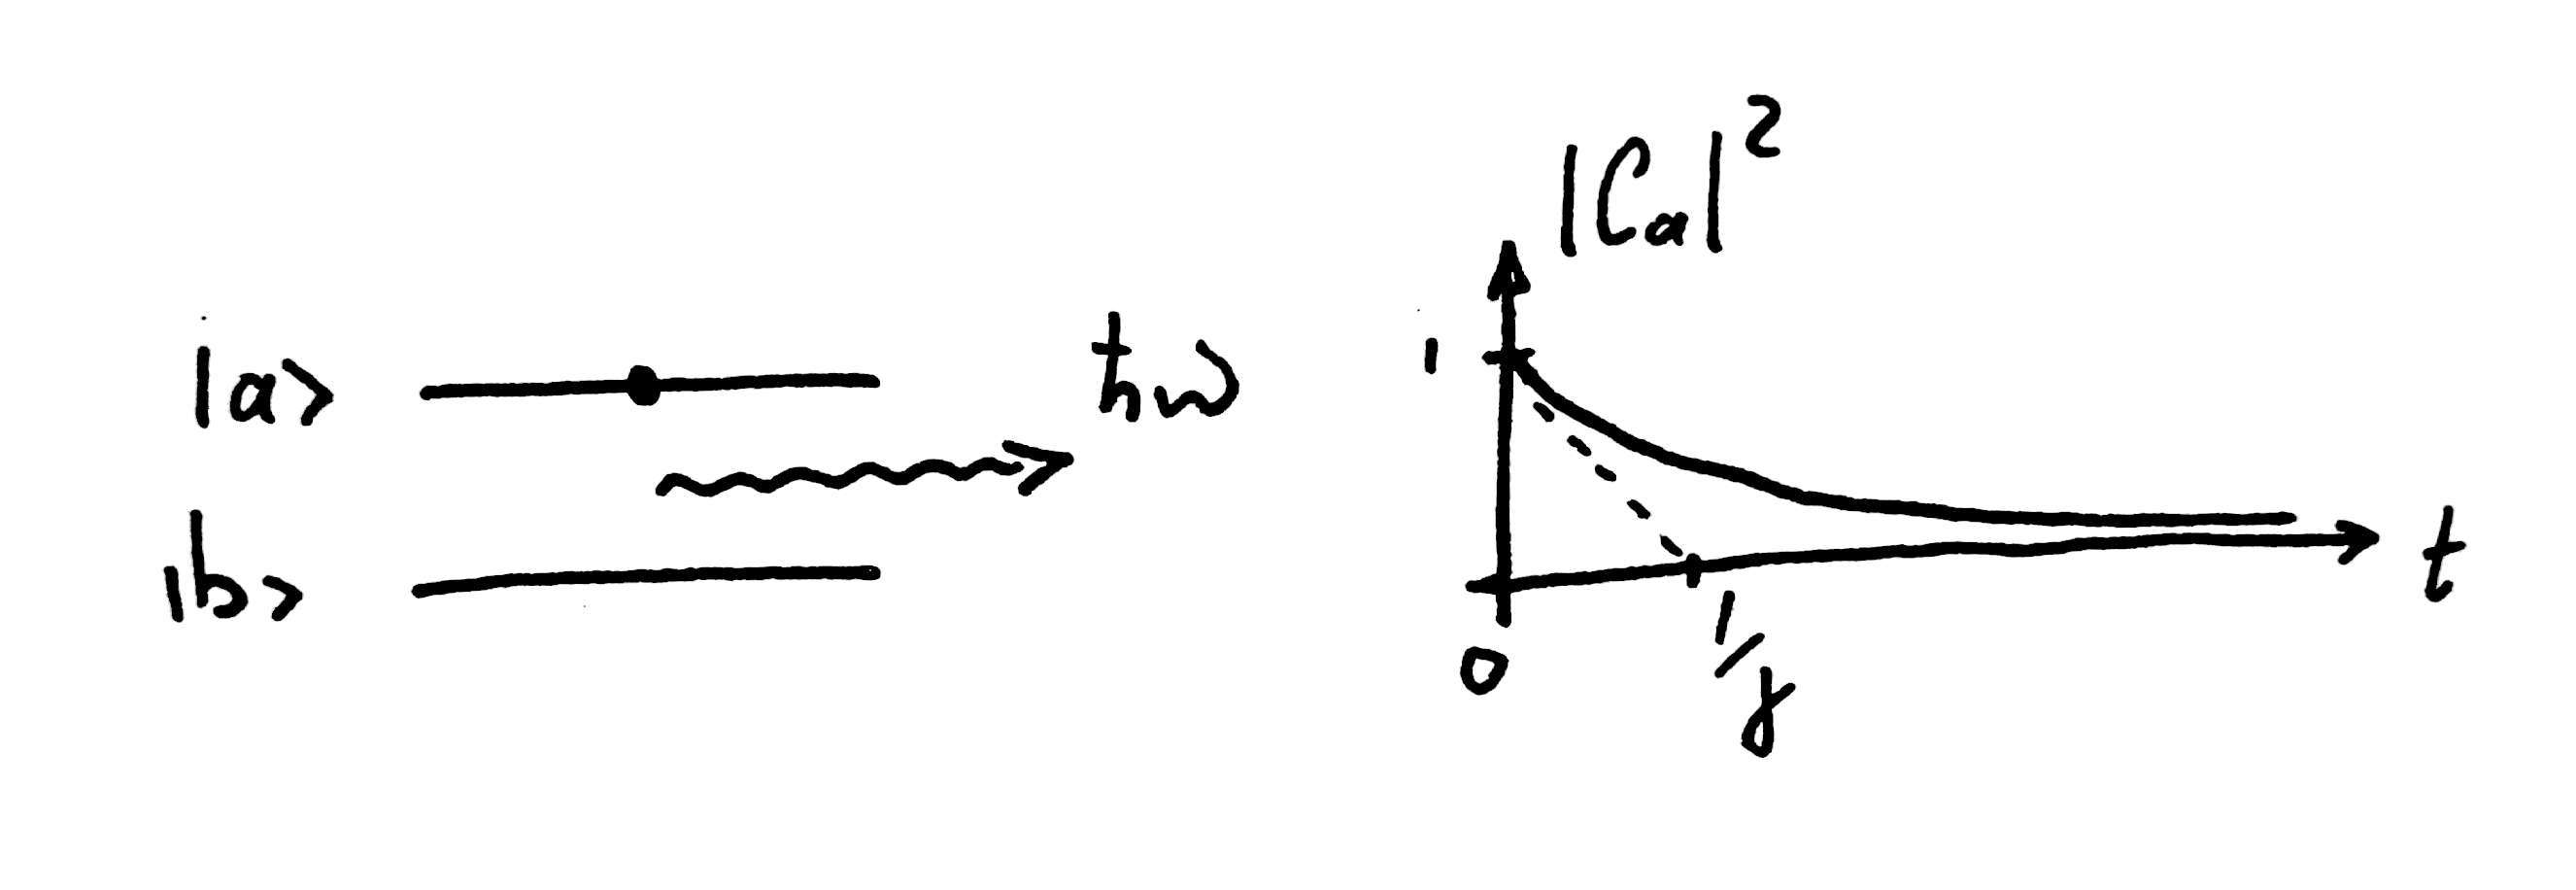
\includegraphics[width=0.65\linewidth]{fig/L7/emissions}
	\caption{Relaxation process}
	\label{fig:emission}
\end{figure}

It is useful to remember that $\gamma \sim n |\vec{d}|^2$ and expression for $\gamma$ contains the Plank constant $\hbar$ which means that this process has a quantum nature.

\textit{Remark:} idea of moves such
\begin{equation}
	\sum_{\kv} \quad \to \quad \int d \omega_{\kv} \quad \to \quad \delta(t - \tau)
\end{equation}
is called the Weisskopf-Wigner method.

In order to compare, when we had a two--level system and a one--mode field we obtained Rabi osculations. In contrast to this, the continuum of modes gives us a relaxation process.   % Scully 6.3
	
	\section{Dipole radiation. Dyadic Green's function. The Purcell effect: classical approach}

\begin{otherlanguage}{russian}	
	\textcolor{red}{На лекциях часть с уравнениями Максвелла была прочитана в СГС, но считаю, что лучше написать это в СИ, так как большинство статей по этой теме и тот же Новотный --- в СИ.}
\end{otherlanguage}

\subsection{Dipole radiation and dyadic Green's function}

Consider a point dipole $\vec{d}_0$ which is located in point $\vec{r}_0$. The electric current is given by
\begin{equation}
	\vec{j} = \rho \vec{v} = \sum_i q_i \delta(\vec{r} - \vec{r}_i) \dot{\vec{r}}_i = \dot{\vec{d}}_0 \delta(\vec{r} - \vec{r}_0).
	\label{eq:dipole_current}
\end{equation}

Let us state a problem to find the dipole field in space. If one wants something which is connected with electromagnetism then he should write Maxwell equations. So we do (in SI units)
\begin{numcases}{}
	\Rot \vec{E} = -  \parder{\vec{B}}{t},
	\label{eq:M1_j} \\
	\Rot \vec{H} = \parder{\vec{D}}{t} + \vec{j},
	\label{eq:M2_j} \\
	\Div \vec{D} = \rho,
	\label{eq:M3_j} \\
	\Div \vec{B} = 0.
	\label{eq:M4_j}
\end{numcases}
After applying the Fourier transform over time (in fact just $\partial_t \to - i \omega$) and using $\vec{D} = \varepsilon \varepsilon_0 \vec{E}$ and $\vec{B} = \mu \mu_0 \vec{H}$  we obtain
\begin{equation}
	\Rot \Rot \vec{E}  - \mu \mu_0 \varepsilon \varepsilon_0 \omega^2 \vec{E} =  i \mu \mu_0 \omega \vec{j}
\end{equation}
introducing $k = \dfrac{\omega}{c} \sqrt{\varepsilon \mu}$ we get
\begin{equation}
	\Rot \Rot \vec{E} - k^2 \vec{E} = \frac{k^2}{\varepsilon \varepsilon_0} \vec{d}_0 \delta(\vec{r} - \vec{r}_0).
	\label{eq:grrr}
\end{equation}
Here we have an inhomogeneous differential equation with a $\delta$--function on the rhs of the equation. Solution of such equation is a Green's function $\hat{\vec{G}}(\vec{r}, \vec{r}_0)$. As \eqref{eq:grrr} is in fact three equation then Green's function for a electromagnetic fields is a tensor or a so--called \textit{dyadic Green's function}. This fact is represent by writing a "hat" over $G$.
 
\subsubsection{Green's function. General information}

A Green's function, $G(x,s)$, of a linear differential operator $\hat{L}$ acting on distributions over a subset of the Euclidean space, at a point s, is any solution of
\begin{equation}
	\hat{L} G(x, s) = \delta(x - s).
\end{equation}
The knowledge of $G(x,s)$ allows us to write the solution in a straight forward way for any rhs part. In other words
\begin{equation}
	\hat{L} u(x) = f(x) \quad \to \quad u(x) = \int ds G(x,s) f(s).
\end{equation}

In our particular case, if we know the radiation of a dipole, we can calculate radiation for any complex current $\vec{j}(\vec{r})$.

\begin{testexample}[Field from an arbitrary current]
	\begin{equation}
		\vec{E}(\vec{r}) = i \begin{pmatrix}
			\dfrac{4 \pi}{c}  \\ \\
			\dfrac{1}{c \varepsilon_0}
		\end{pmatrix} k \int d^3r' \hat{\vec{G}}(\vec{r}, \vec{r}') \vec{j}(\vec{r}'), \qquad \text{units: }\begin{pmatrix}
		\text{sgs}  \\ \\
		\text{SI}
		\end{pmatrix}
		\label{eq:E_from_G}
	\end{equation}
	\textit{Remark:} $\hat{\vec{G}} \vec{j} = \vec{e}_i \hat{G}_{ik} j_k$, where $\vec{e}_i$ --- a unit vector.
\end{testexample}

\subsubsection{Derivation of the Green's function for Maxwell equations}

As we understand how it is convenient and important, let us find the explicit form for $\hat{\vec{G}}$. The general definition of the dyadic Green’s function for the electric field is
\begin{equation}
	\Rot \Rot \hat{\vec{G}}(\vec{r}, \vec{r}_0) - k^2 \hat{\vec{G}}(\vec{r}, \vec{r}_0) = \hat{\vec{I}} \delta(\vec{r} - \vec{r}_0).
\end{equation}
If we know $\hat{\vec{G}}$, then we know $\vec{E}$ from \eqref{eq:E_from_G}. On the other hand we know that
\begin{equation}
	\vec{E} = - \nabla \varphi - \parder{\vec{A}}{t}.
	\label{eq:elll}
\end{equation}
If we use electromagnetic potential $\vec{A}$ then we can choose any gauge for our convenience. Let us take the Lorenz gauge
\begin{equation}
	\Div \vec{A} + \frac{1}{c} \parder{\varphi}{t} = 0 \quad \to \quad \nabla \varphi = \frac{c}{i \omega} \nabla \Div \vec{A}.
\end{equation}
It means that $\varphi$ and $\vec{A}$ obeys
\begin{numcases}{\label{eq:gelm}}
	\Delta \vec{A} + k^2 \vec{A} = - \mu \mu_0 \vec{j}, \\
	\Delta \varphi + k^2 \varphi = - \frac{\rho}{\varepsilon \varepsilon_0}.	
\end{numcases}
As we can see \eqref{eq:gelm} ---inhomogeneous Helmholtz equations. The Green's function is known (careful derivation is too long and may take away from the main point):
\begin{equation}
	G_0(\vec{r}, \vec{r}_0) = \frac{e^{ikR}}{4\pi R}, \qquad R = \left| \vec{r} - \vec{r}_0 \right|.
\end{equation}
It means that we can write the solution of \eqref{eq:gelm} as
\begin{numcases}{\label{eq:solll}}
	\vec{A}(\vec{r}) = \mu \mu_0 \int d^3 r' G_0(\vec{r}, \vec{r}') \hat{\vec{I}} \vec{j}(\vec{r}'), \\
	\varphi(\vec{r}) = \frac{1}{\varepsilon \varepsilon_0} \int d^3r' G_0(\vec{r}, \vec{r}') \rho(\vec{r}'),
\end{numcases}
where $\hat{\vec{I}}_{ik} = \delta_{ik}$ --- a unit tensor. To get the final answer for $\hat{\vec{G}}$ we substitute \eqref{eq:solll} in \eqref{eq:elll} and compare the result with \eqref{eq:E_from_G}. Substitution gives
\begin{equation}
	\vec{E}(\vec{r}) = i \omega \mu \mu_0 \int d^3 r' \underbrace{\left[ G_0(\vec{r}, \vec{r}') \hat{\vec{I}} + \frac{1}{k^2} \nabla \Div G_0(\vec{r}, \vec{r}') \hat{\vec{I}} \right]}_{\hookrightarrow \myeq \hat{\vec{G}}(\vec{r}, \vec{r}')} \vec{j}(\vec{r}')
\end{equation}
or
\begin{equation}
	\hat{\vec{G}}(\vec{r}, \vec{r}_0) = \left( \hat{\vec{I}} + \frac{1}{k^2} \nabla \otimes \nabla \right) G_0(\vec{r}, \vec{r}_0),
	\label{eq:ggGGGgg}
\end{equation}
where $(\nabla \otimes \nabla)_{\alpha \beta} = \partial_{\alpha} \partial_{\beta}$, $\alpha, \beta = x,y,z$ --- a tensor product of $\nabla$.
 
\begin{testexample}[Field of a point dipole in vacuum]
	Let us assume a monochromic dipole, so from \eqref{eq:dipole_current} we obtain
	\begin{equation}
		\vec{j} = -i\omega \vec{d}_0 \delta(\vec{r} - \vec{r}_0).
	\end{equation}
	Substitution to \eqref{eq:E_from_G} gives
	\begin{equation}
		\vec{E}(\vec{r}) = i \frac{4\pi}{c}k (-i\omega) \int d^3 r' \hat{\vec{G}}(\vec{r}, \vec{r}') \vec{d}_0 \delta(\vec{r} - \vec{r}_0) = 4\pi k^2 \hat{\vec{G}}(\vec{r}, \vec{r}_0) \vec{d}_0
	\end{equation}
	or
	\begin{equation}
		E_{\alpha}(\vec{r}) = 4\pi k^2  \hat{G}_{\alpha \beta}(\vec{r}, \vec{r}_0) d_{0 \beta} \quad \text{(sgs)}.
	\end{equation}
	\textit{Remark:} interesting to notice that is $\vec{d}_0 = (d_0,0,0)$ then the first column of $\hat{\vec{G}}$ shows a field which induces a dipole $Ox$-directed.
\end{testexample}

\subsubsection{Near-, intermediate- and far-field parts of Green's function}

Sometimes it is convenient to write  \eqref{eq:ggGGGgg} in different form:
\begin{equation}
	\hat{\vec{G}}(\vec{r}, \vec{r}_0) \overset{\vec{R} = \vec{r} - \vec{r}_0}{=} \hat{\vec{G}}(\vec{R}) = \hat{\vec{G}}_{NF} + \hat{\vec{G}}_{IF} + \hat{\vec{G}}_{FF},
\end{equation}
where
\begin{equation*}
	\begin{matrix}
		(\text{electrostatics}) & \hat{\vec{G}}_{NF} &=& \frac{e^{ikR}}{4\pi R} \frac{1}{k^2R^2} \left( 3 \frac{\vec{R}\otimes\vec{R}}{R^2} - \hat{\vec{I}} \right), & kR \ll 1 \\ \\
		& \hat{\vec{G}}_{IF} &=& \frac{e^{ikR}}{4\pi R} \frac{i}{kR}  \left( \hat{\vec{I}} - 3\frac{\vec{R}\otimes\vec{R}}{R^2} \right), & kR \sim 1 \\ \\
		(\text{electrodynamics})& \hat{\vec{G}}_{FF} &=& \frac{e^{ikR}}{4\pi R}  \left( \hat{\vec{I}} - \frac{\vec{R}\otimes\vec{R}}{R^2} \right), & kR \gg 1
	\end{matrix}
\end{equation*}
  % Novotny 2.10
	
	\section{Theory of relaxation of electromagnetic filed. Heisenberg--Langevin method}

\subsection{In previous series}

We have discussed:
\begin{enumerate}
	\item Two-level system (e.g. atom) and one mode field. Result: Rabi oscillations.
	\item Two-level system and continuum of modes (e.g. cavity). Result: spontaneous emission.
	\item One-mode field in the cavity and continuum of modes. Result: let's find out!
\end{enumerate}

\begin{figure}[h!]
	\centering
	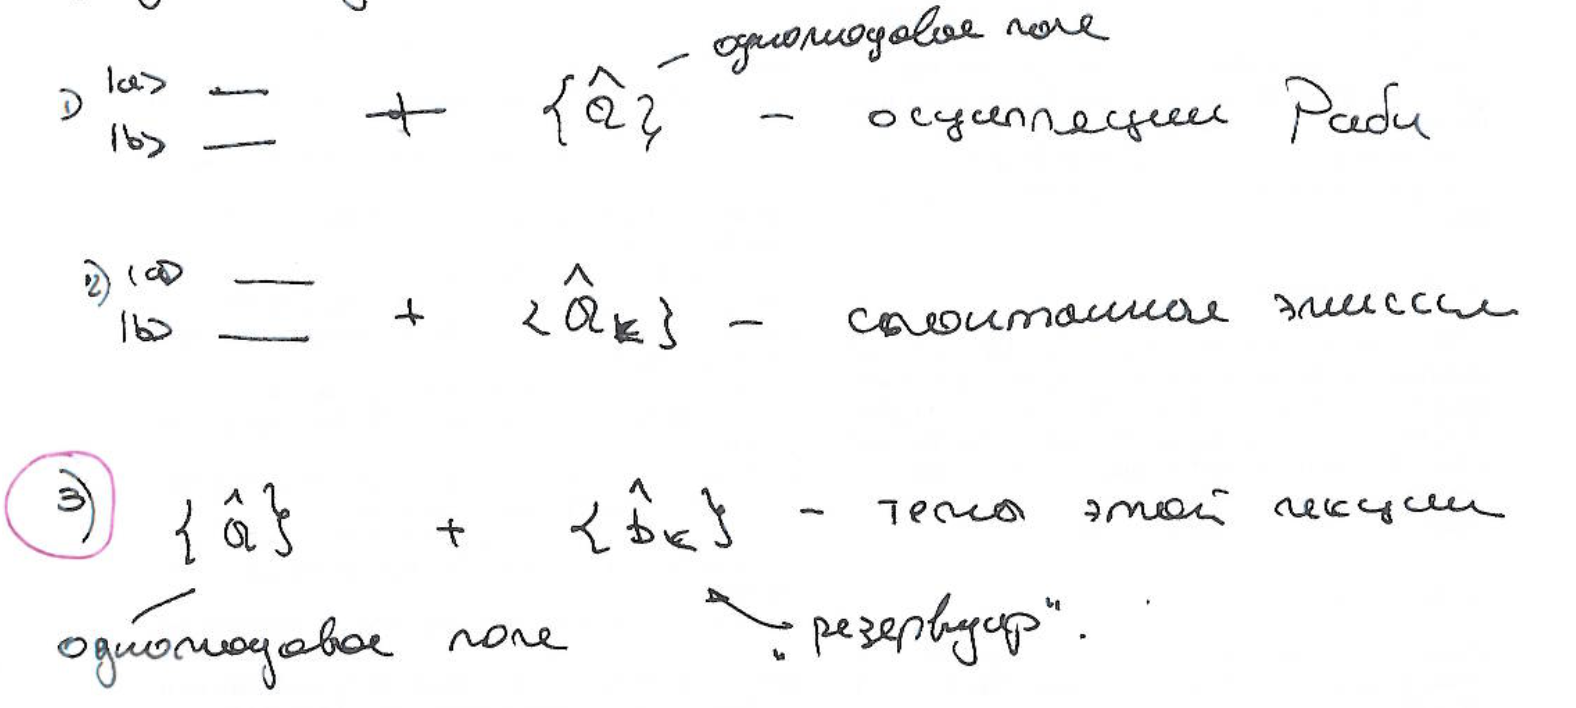
\includegraphics[width=0.8\linewidth]{fig/L9/fig1}
	\caption{Different possible cases for analytical consideration.}
	\label{fig:fig11}
\end{figure}

\subsection{the Heisenberg--Langevin equation}

We are interested in dynamics of $\hat{b}(t)$ and $\hat{a}(t)$ in thermodynamics equilibrium at the temperature $T$. We consider modes which are fluctuate independently
\begin{eqnarray}
	\left \langle \hat{b}^{\dagger}_{\kv} (0) \hat{b}_{\kv'} (0) \right \rangle &=& \bar{n}_{\kv} \delta_{\vec{k}\vec{k}'}, \\
	\av{\hat{b}_{\kv}(0)} = \av{\hat{b}^{\dagger}_{\kv}(0)} &=& 0,\\
	\av{\hat{b}_{\kv} (0) \hat{b}^{\dagger}_{\kv'} (0) } &=& (\bar{n}_{\kv}+1) \delta_{\vec{k}\vec{k}'}, \\
	\av{\hat{b}_{\kv} (0) \hat{b}_{\kv'} (0) } = \av{\hat{b}^{\dagger}_{\kv} (0) \hat{b}^{\dagger}_{\kv'} (0) } &=& 0.
\end{eqnarray}
Here and  hereinafter the angle brakes represent the reservoir averages $\av{\dots} \equiv \av{\dots}_{\text{R}}$.

As the wave function is unknown we use the density matrix approach. Density matrix and distribution function in thermodynamics equilibrium is given by
\begin{equation}
	\rho_R = \Pi \left( 1 - e^{- \frac{\hbar \omega_{\vec{k}}}{kT}} \right) e^{- \frac{\hbar \omega_{\vec{k}} \hat{b}_{\kv}^{\dagger} \hat{b}_{\kv}}{kT}}, \qquad \bar{n}_{\kv}  = \frac{1}{e^{\frac{\hbar \omega_{\vec{k}}}{kT}} - 1}.
\end{equation}
The Hamiltonian of the system can be written as 
\begin{equation}
	\hat{\mathcal{H}} = \underbrace{\hbar \omega \hat{a}^{\dagger} \hat{a}}_{\text{resonator}} + \underbrace{\sum_{\kv} \hbar \omega_{\kv} \hat{b}^{\dagger}_{\kv} \hat{b}_{\kv}}_{\text{cavity}} + \underbrace{\sum_{\kv} \hbar  \left( g_{\kv} \hat{b}_{\kv}^{\dagger} \hat{a}_{\kv} + g^*_{\kv} \hat{a}_{\kv}^{\dagger} \hat{b}_{\kv}  \right)}_{\hat{\mathcal{H}}_{\text{int}}}.
\end{equation}
The  explicit form of $g_{\kv}$ is strongly depend on exact system. However we know the asymptotic behavior --- if the resonator is ideal then $g_{\kv} = 0$.

Time evolution is defined by
\begin{equation}
	\hat{\dot{a}}(t) = \frac{i}{\hbar} \left[ \hat{\mathcal{H}}, \hat{a}  \right], \qquad  	\hat{\dot{b}}(t) = \frac{i}{\hbar} \left[ \hat{\mathcal{H}}, \hat{b}  \right],
\end{equation} 
which gives 
\begin{numcases}{}
		\hat{\dot{a}}(t) = -i \omega \hat{a}(t) - i \sum_{\kv} g_{\kv}^* \hat{b}_{\kv}(t), \label{eq:a_dyn}\\
		\hat{\dot{b}}_{\kv}(t) = -i \omega_{\kv} \hat{b}_{\kv}(t) - i  g_{\kv} \hat{a}(t),
		\label{eq:b_dyn}
\end{numcases}
Important to notice that it is sensible to consider only the mean values of operators. 

Now let us solve this system. it is easy to verify that the solution of  \eqref{eq:b_dyn}  is
\begin{equation}
	\hat{b}_{\kv}(t) = \underbrace{\hat{b}_{\kv}(0) e^{-i\omega_{\kv} t}}_{\text{reservoir modes evolution}} - \underbrace{i g_{\kv} \int \limits_0^{t} d\tau \hat{a}(\tau) e^{-i\omega_{\kv}(t - \tau)}}_{\text{interaction between reservoir and oscillator}}
\end{equation}
then we substitute this result in \eqref{eq:a_dyn} and obtain
\begin{equation}
	\hat{\dot{a}}(t) = - i \omega \hat{a}(t) - \hat{f}_a(t) + \sum_{\kv} \left| g_{\kv} \right|^2 \int \limits_0^td\tau \hat{a}(\tau) e^{-i\omega_{\kv}(t - \tau)},
\end{equation}
where
\begin{equation}
	\hat{f}_a(t) \myeq i \sum_{\kv} g_{\kv}^* \hat{b}_{\kv}(0) e^{-i\omega_{\kv} t}
\end{equation}
is a stochastic operator as the number of photons in a particular time moment is undefined. After that we introduce 
\begin{equation}
	\hat{\tilde{a}}(t) \myeq \hat{a}(t) e^{i \omega t}, \qquad \hat{F}_{\tilde{a}} (t) = \hat{f}_a(t) e^{i \omega t}
\end{equation}
and obtain \textit{a stochastic integro-differential equation} 
\begin{equation}
	\hat{\dot{\tilde{a}}}(t) = \sum_{\kv} \left| g_{\kv} \right|^2 \int \limits_0^t d\tau \hat{\tilde{a}} e^{i(\omega-\omega_{\kv})(t - \tau)} + \hat{F}_{\tilde{a}} (t).
	\label{eq:st_int_dif}
\end{equation}
which is quite hard to solve, unless one was educated in the USSR.

To find a solution of \eqref{eq:st_int_dif} we, first of all, make transition from sum to the integral
\begin{equation}
	\sum_{\kv} \left| g_{\kv} \right|^2 \quad \to \quad \frac{V}{\pi^2 c^3} \int \limits_0^{\infty} d \omega_{\kv} \omega_{\kv}^2 \left| g_{\omega_{\kv}} \right|^2.
\end{equation}
Now let us consider only the integral in \eqref{eq:st_int_dif} which becomes
\begin{multline}
	\frac{V}{\pi^2 c^3} \int \limits_0^{\infty} d \omega_{\kv} \omega_{\kv}^2 \left| g_{\omega_{\kv}} \right|^2 \int \limits_0^t d\tau \hat{\tilde{a}}(\tau)e^{i(\omega - \omega_{\kv})(t - \tau)} = \\ =\Bigg/ \omega_{\kv}^2 \left| g_{\omega_{\kv}} \right|^2 \text{ is a slow function} \Bigg/
	\approx \frac{V}{\pi^2 c^3} \int \limits_0^t d \tau \hat{\tilde{a}}(\tau) \cdot \omega_{\kv}^2 \left| g_{\omega_{\kv}} \right|^2 \cdot  \underbrace{\int \limits_0^{\infty} d \omega_{\kv} e^{i(\omega - \omega_{\kv})(t - \tau)}}_{\hookrightarrow\approx 2\pi \delta(t - \tau)} =\\= \frac{V}{\pi^2 c^3} \omega_{\kv}^2 \cdot 2 \pi \left| g_{\omega_{\kv}} \right|^2 \underbrace{\int \limits_0^t d\tau \hat{\tilde{a}}(\tau) \delta(t - \tau)}_{\half \hat{\tilde{a}}(t)}  =\frac{\Gamma}{2}\hat{\tilde{a}}(t),
\end{multline}
where we defined a relaxation constant $\Gamma$ and density of states $D$:
\begin{equation}
	\Gamma \myeq D(\omega_{\kv}) \cdot 2 \pi \left| g_{\omega_{\kv}} \right|^2  , \qquad D(\omega_{\kv}) = \frac{V \omega_{\kv}^2}{\pi^2 c^3} = \int d^3 r \rho(\vec{r}, \omega_{\kv}).
\end{equation}
So finally here is \textit{the Heisenberg--Langevin equation}:
\begin{equation}
	\boxed{\hat{\dot{\tilde{a}}}(t) = - \frac{\Gamma}{2} \hat{\tilde{a}}(t) + \hat{F}_{\tilde{a}} (t). }
	\label{eq:HLeq}
\end{equation}

\textit{Remark:} we could obtain the same result if we would have considered the dynamics of atom's operator $\hat{\dot{\sigma}}_z(t)$.

\begin{testexample}[Connection between dissipation and fluctuation]
	Let us put $\hat{F}_{\tilde{a}} (t) = 0$. It means that $\hat{\tilde{a}}(t) = \hat{\tilde{a}}(0) e^{- \frac{\Gamma}{2} t}$ which leads to
	\begin{equation}
		\left[ \hat{\tilde{a}}(t), \hat{\tilde{a}}^{\dagger}(t) \right] = e^{- \Gamma t} \neq 1.
		\label{eq:example}
	\end{equation}
	That is nonsense! It couldn’t be, so we can not just put the stochastic term to zero. \textit{If there is a dissipation then there have to be fluctuation in the system.}
\end{testexample}

\subsection{Properties of the stochastic operator}

Let us find out properties of the stochastic operator $\hat{F}_a(t)$. The mean values are
\begin{equation}
	\av{\hat{F}_a(t)} = \av{\hat{F}_a^{\dagger}(t)} = 0.
\end{equation}
Now let us find the correlator
\begin{multline}
	\av{\hat{F}_a^{\dagger}(t) \hat{F}_a(t')} = \sum_{\kv \kv'} g^*_{\kv} g_{\kv'} \underbrace{\cdot \av{\hat{b}_{\kv}^{\dagger}(0) \hat{b}_{\kv}(0)} \cdot }_{\overset{\hookrightarrow=\bar{n}_{\kv} \delta_{\vec{k}\vec{k}'}}{\text{av. num. of ph. in } \kv}} e^{i(\omega_{\kv} - \omega)t - i(\omega_{\kv'} - \omega)t'} = \\ 
	= \sum_{\kv} \left| g_{\kv}\right|^2 \bar{n}_{\kv} e^{i (\omega_{\kv} - \omega)(t - t')} = \int \limits_0^{\infty} d \omega_{\kv} D(\omega_{\kv}) \left| g_{\kv}\right|^2 \bar{n}_{\kv} (\omega_{\kv}) e^{i (\omega_{\kv} - \omega)(t - t')} \approx \\ \approx \underbrace{D(\omega_{\kv}) \left| g_{\kv}\right|^2 \bar{n}_{\kv} (\omega_{\kv})}_{\text{slow func}} \cdot 2\pi \delta(t-t'),
\end{multline}
so we have
\begin{equation}
	\av{\hat{F}_a^{\dagger}(t) \hat{F}_a(t')} = \bar{n}_{\kv} \Gamma \delta(t - t').
	\label{eq:111jhh}
\end{equation}
Any stochastic function with $\delta$--shaped correlator is called \textit{white noise}. After integration over $t'$ in \eqref{eq:111jhh} the dissipation rate  can be written as
\begin{equation}
	\boxed{\Gamma = \frac{1}{\bar{n}_{\kv}(\omega_{\kv})} \int \limits_{-\infty}^{\infty} dt' \av{\hat{F}_a^{\dagger}(t) \hat{F}_a(t')}.}
\end{equation}
This relation takes it roots from the \textit{fluctuation-dissipation theorem}.

Consider another averaging, that is the average of stochastic operator and an annihilation operator $\av{\hat{F}_a^{\dagger}(t) \hat{\tilde{a}}(t)}$.
From \eqref{eq:HLeq} we get
\begin{equation}
	\hat{\tilde{a}}(t) = \hat{\tilde{a}}(0) e^{- \frac{\Gamma}{2}t} + \int \limits_0^t  d \tau \hat{F}_a(\tau)e^{- \frac{\Gamma}{2}(t - \tau)},
\end{equation}
so
\begin{equation}
	\av{\hat{F}_a^{\dagger}(t) \hat{\tilde{a}}(t)} = \underbrace{\av{\hat{F}_a^{\dagger}(t) \hat{\tilde{a}}(0)e^{- \frac{\Gamma}{2}t}}}_{\hookrightarrow=0, \text{ as } \av{\hat{F}_a}=0} + \int \limits_0^t d\tau \av{\hat{F}_a^{\dagger}(t) \hat{F}_a(\tau)} e^{- \frac{\Gamma}{2}(t - \tau)} \overset{\eqref{eq:111jhh}}{=} \frac{\bar{n}_{\kv}\Gamma}{2}.
\end{equation}
In a similar way it is easy to get the same result for $\av{\hat{\tilde{a}}(t) \hat{F}_a^{\dagger}(t) }$, so we can write
\begin{equation}
	\boxed{	\av{\hat{F}_a^{\dagger}(t) \hat{\tilde{a}}(t)} = \av{\hat{\tilde{a}}(t) \hat{F}_a^{\dagger}(t) } =  \frac{\bar{n}_{\kv}\Gamma}{2}.}
	\label{eq:heeeelp}
\end{equation}

These correlation functions will be employed to derive equations of motion for the field correlation functions.

\subsection{Equation of motion for the field correlation functions. Wiener--Khintchine theorem}

The mean time development of the field number operator is
\begin{multline}
	\frac{d}{dt} \av{\hat{\tilde{a}}^{\dagger}(t) \hat{\tilde{a}}(t)}  = \av{ \frac{d\hat{\tilde{a}}^{\dagger}}{dt} \hat{\tilde{a}}} + \av{\hat{\tilde{a}}^{\dagger} \frac{d\hat{\tilde{a}}}{dt}} \overset{\eqref{eq:HLeq}}{=} - \frac{\Gamma}{2} \av{\hat{\tilde{a}}^{\dagger} \hat{\tilde{a}}} + \underbrace{\av{\hat{F}_a^{\dagger} \hat{\tilde{a}}} + \av{\hat{\tilde{a}} \hat{F}_a^{\dagger}}}_{\hookrightarrow \overset{\eqref{eq:heeeelp}}{=} \Gamma \bar{n}_{\kv}}  - \frac{\Gamma}{2} \av{\hat{\tilde{a}}^{\dagger} \hat{\tilde{a}}} = \\ = - \Gamma \av{\hat{\tilde{a}}^{\dagger} \hat{\tilde{a}}} + \Gamma \bar{n}_{\kv}.
	\label{eq:dn}
\end{multline}
In a similar manner, it can be shown that
\begin{equation}
	\frac{d}{dt} \av{\hat{\tilde{a}}(t) \hat{\tilde{a}}^{\dagger}(t)} = - \Gamma \av{\hat{\tilde{a}} \hat{\tilde{a}}^{\dagger}} + \Gamma \left(\bar{n}_{\kv}+1\right).
\end{equation}

To verify our results let us find the same commutator which was found in the example above. Shall we start with
\begin{equation}
	\frac{d}{dt} \av{\left[ \hat{\tilde{a}}(t), \hat{\tilde{a}}^{\dagger}(t) \right]} = \Gamma \left( 1 - \av{\left[ \hat{\tilde{a}}(t), \hat{\tilde{a}}^{\dagger}(t) \right]} \right).
\end{equation}
We now what value should be at time $t=0$, in other words we know the initial conditions for this differential equation, so letting $\zeta \myeq \av{\left[ \hat{\tilde{a}}(t), \hat{\tilde{a}}^{\dagger}(t) \right]}$, we have
\begin{equation}
	\begin{cases}
		\dot{\zeta} = \Gamma (1 - \xi) \\
		\zeta_{\ t=0} = 1
	\end{cases}
	\quad \to \quad \zeta = 1 \quad \to \quad \boxed{\av{\left[ \hat{\tilde{a}}(t), \hat{\tilde{a}}^{\dagger}(t) \right]} = 1.}
\end{equation}
Which is correct in contrast to \eqref{eq:example}.

To define the spectrum we need to use \textit{the Wiener--Khintchine theorem}. In short, this theorem allows to find spectrum using the knowledge of the correlation function (fig. \ref{fig:wiener}) using relation
\begin{equation}
	S_f(\omega) = \frac{1}{\pi} \int \limits_{-\infty}^{\infty} d \tau e^{-i \omega \tau} \cdot \av{f^*(t) f(t + \tau)} 
\end{equation}
\begin{otherlanguage}{russian}	
	\textcolor{red}{Спектр написал, как было на лекциях, хотя в Скалли (ур-е 9.3.11) немного другое выражение, там $\int_0^{\infty}$ и берут действительную часть от интеграла.}
\end{otherlanguage}

\begin{figure}
	\centering
	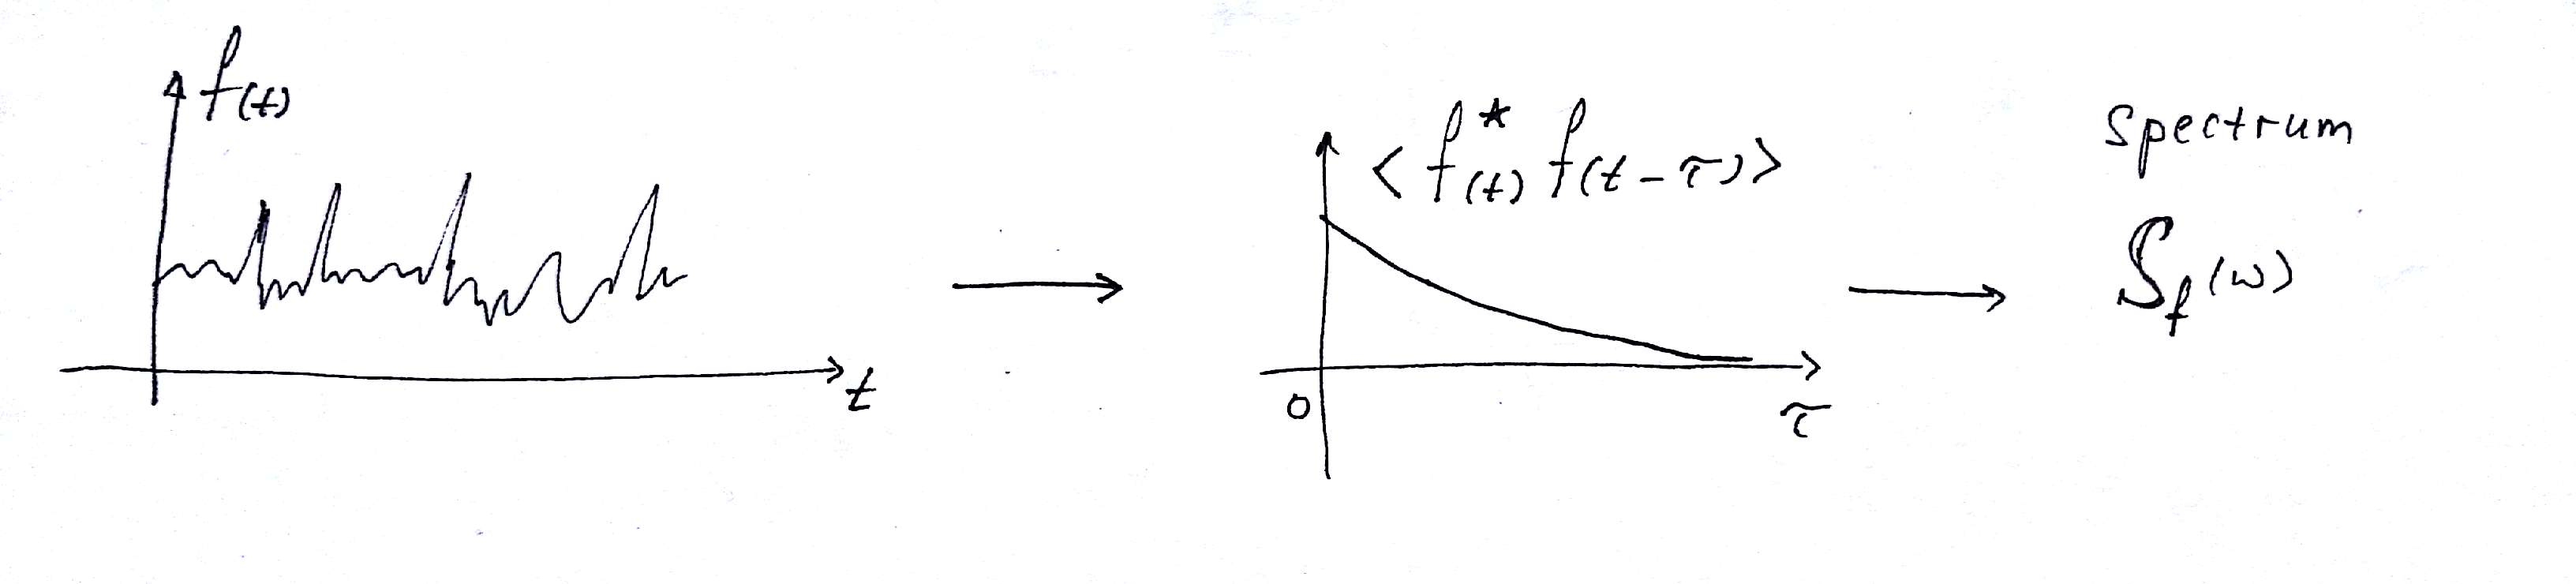
\includegraphics[width=0.85\linewidth]{fig/L9/wiener}
	\caption{Wiener--Khintchine theorem in 40 seconds}
	\label{fig:wiener}
\end{figure}

In our case instead of $f(t)$ we have $ \hat{a}(t) = \hat{\tilde{a}}(t) e^{-i \omega t}$ which gives
\begin{equation}
	\av{\hat{a}^{\dagger}(t_0) \hat{a}(t_0 + \tau)} = \av{\hat{\tilde{a}}^{\dagger}(t_0) \hat{\tilde{a}}(t_0 + \tau)} e^{- i \omega \tau} = \av{n} e^{- \frac{\Gamma\tau}{2}} e^{-i\omega \tau},
\end{equation}
where $\av{n} \myeq  \av{\hat{\tilde{a}}^{\dagger}(t_0) \hat{\tilde{a}}(t_0)}$ is the mean number of photons at the initial time $t_0$. Then the spectrum
\begin{equation}
	S(\nu) = \frac{1}{\pi} \av{n}  \int \limits_{-\infty}^{\infty} d \tau e^{-i \nu \tau} \cdot e^{- \frac{\Gamma\tau}{2}} e^{-i\omega \tau} = \frac{1}{\pi} \av{n} \frac{\Gamma/2}{\left( \nu - \omega \right)^2 + \left(\Gamma/2\right)^2}.
\end{equation}
This is a Lorentzian distribution centered at $\nu = \omega$ with a half--width $\Gamma$ (fig. \ref{fig:loren}). The quality factor is connected with our results and can be written as $Q = \frac{\omega}{\Gamma}$.

\begin{figure}[h!]
	\centering
	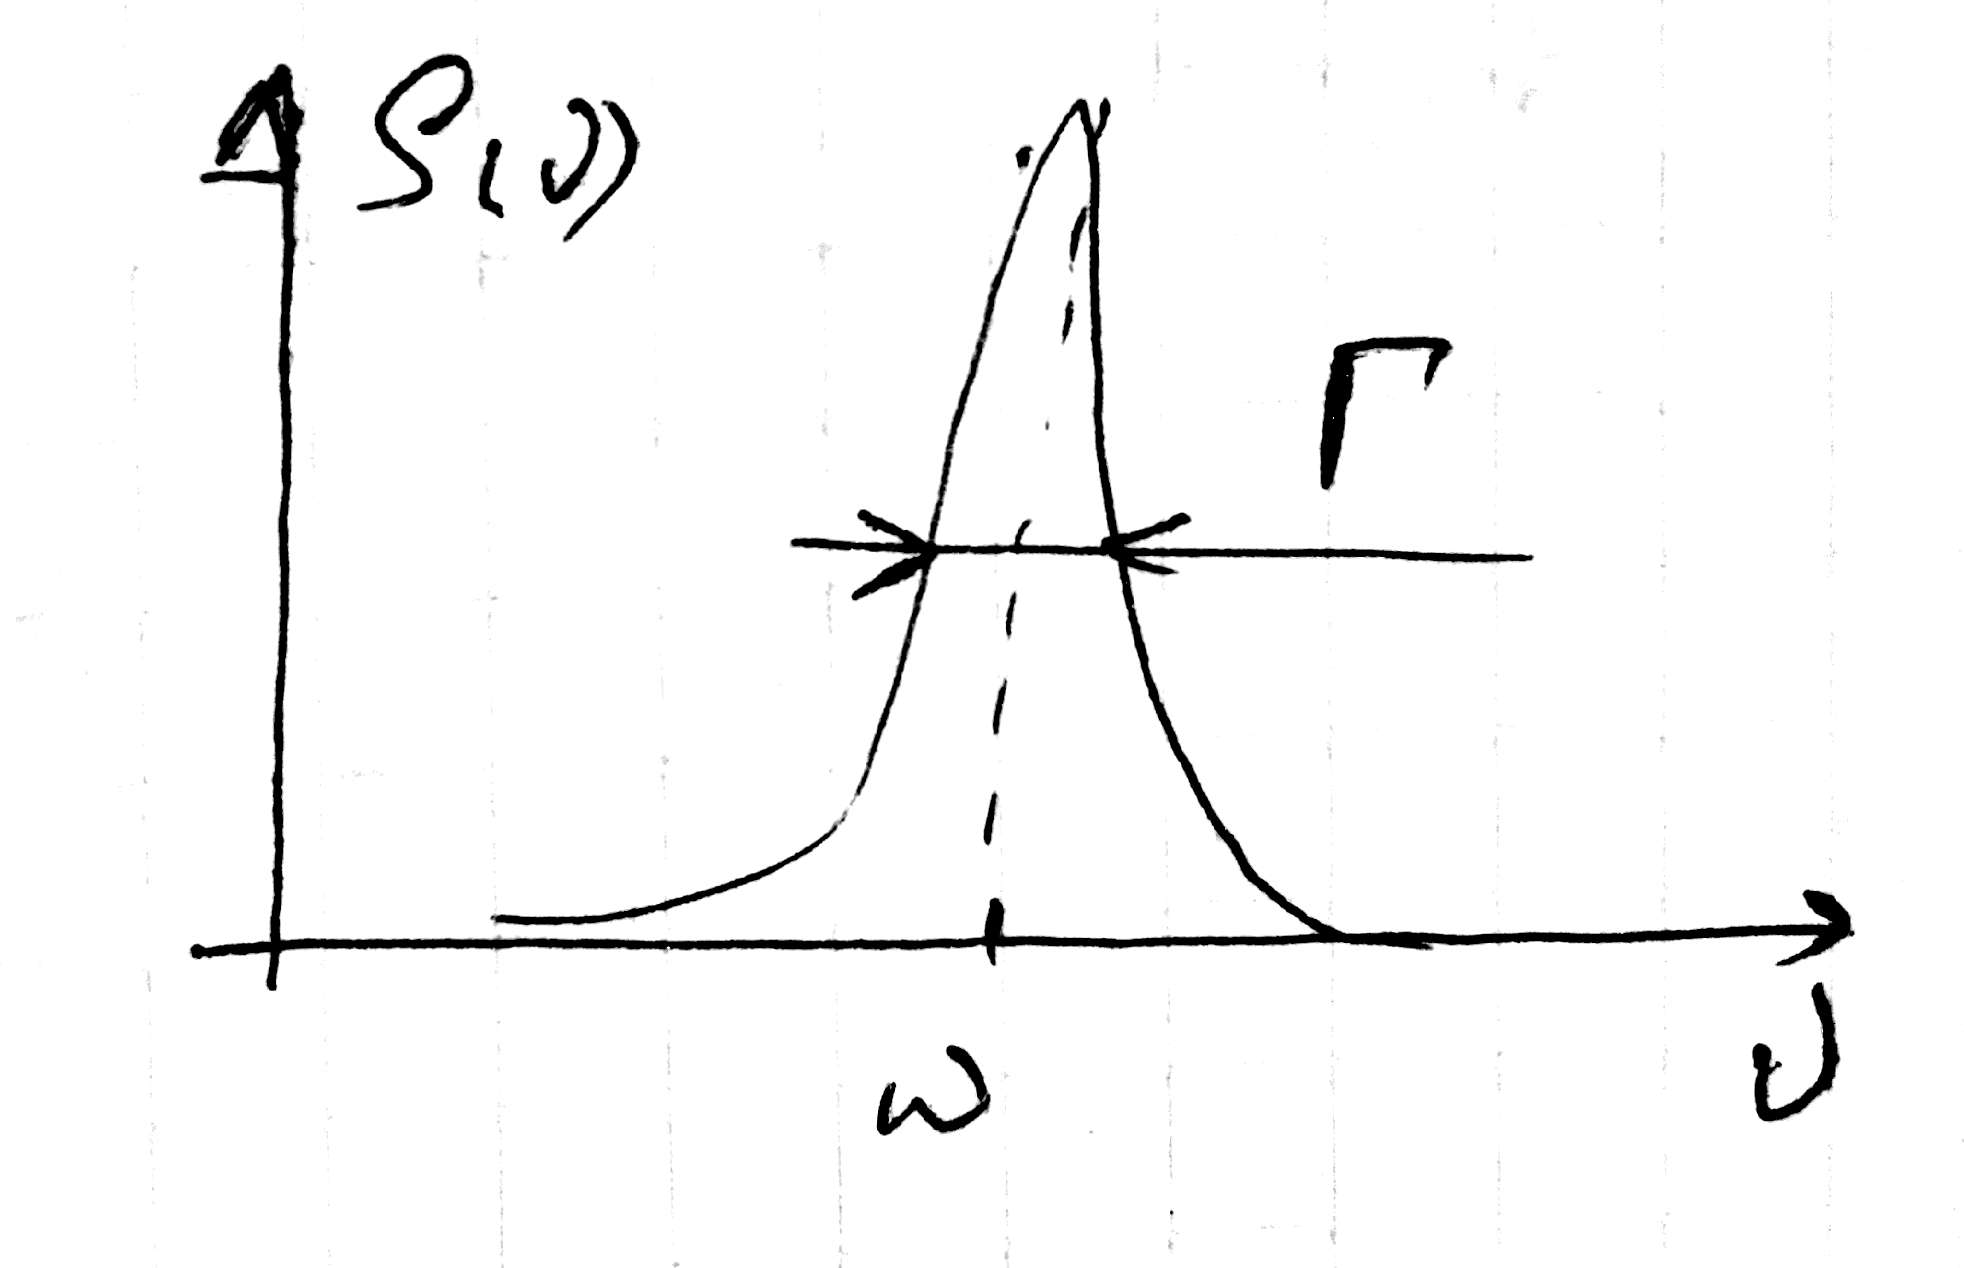
\includegraphics[width=0.4\linewidth]{fig/L9/L_1}
	\caption{Spectrum has a Lorentzian distribution shape}
	\label{fig:loren}
\end{figure}

	
	\section{Atom in a damped cavity}

In the previous sections we have discussed different parts of the system (fig. \ref{fig:before}) which we are going to combine in this section.

\begin{figure}[h!]
	\centering
	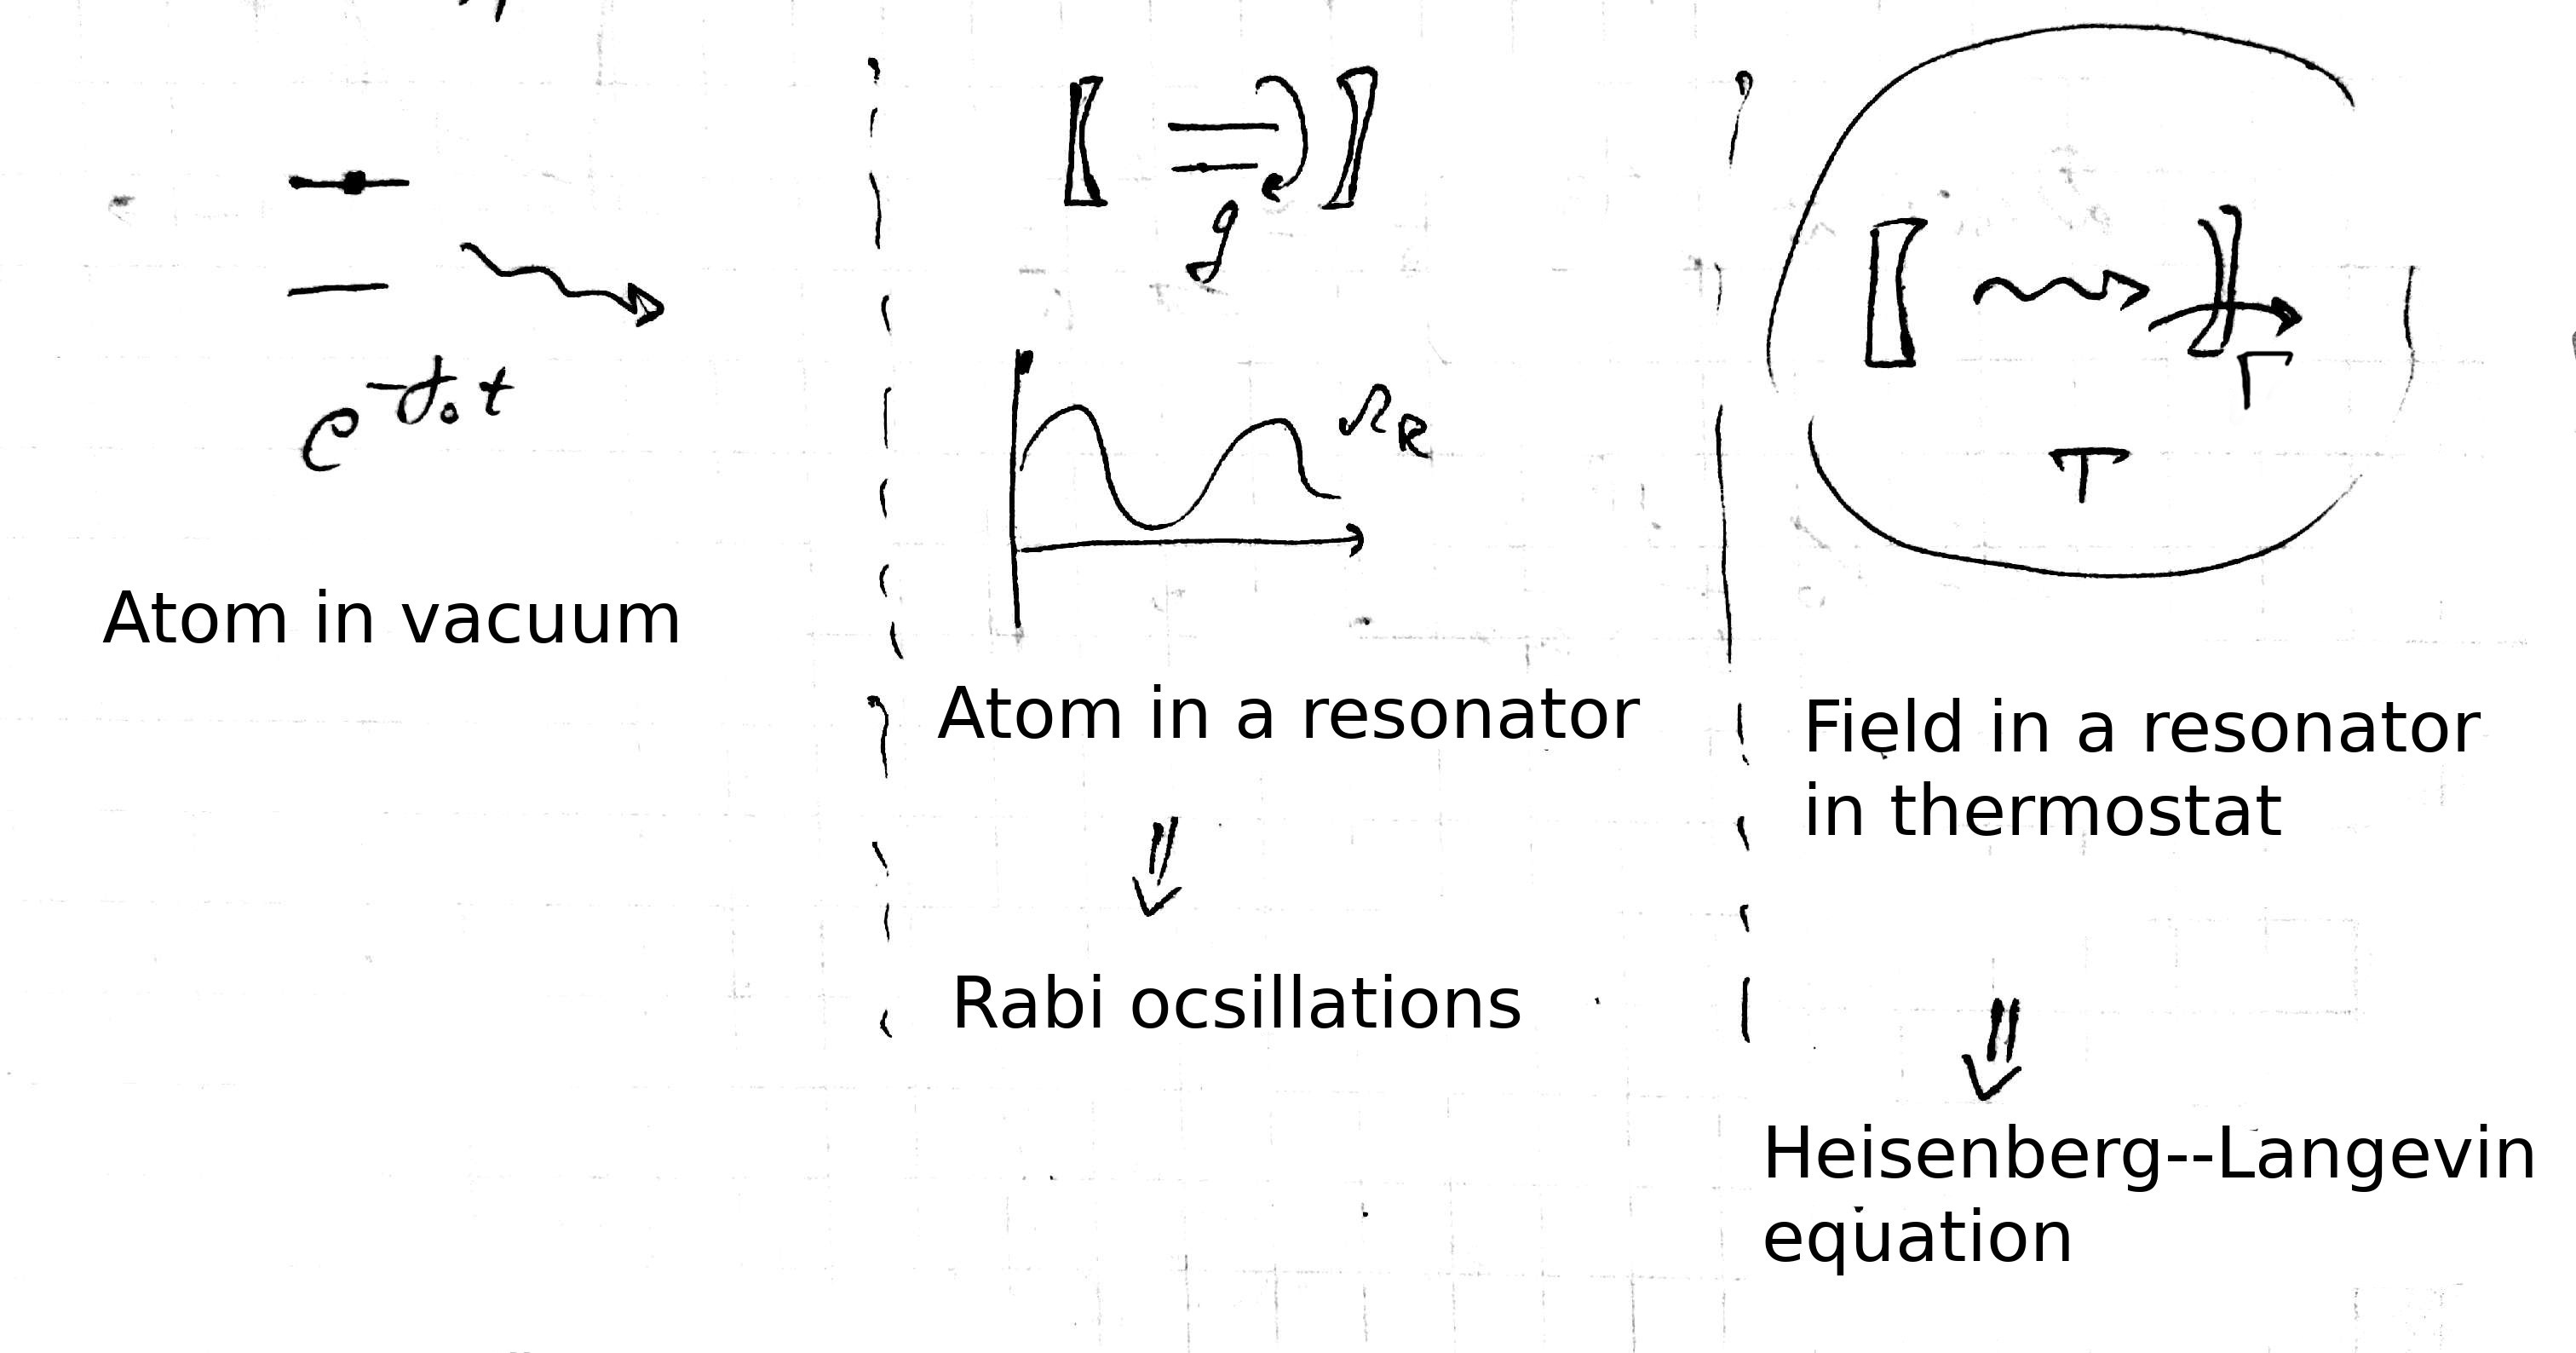
\includegraphics[width=0.7\linewidth]{fig/L10/before}
	\caption{From left to right: atom in vacuum, atom in the cavity, field in a cavity in a thermostat.}
	\label{fig:before}
\end{figure}


Here we are going to study the evolution of a single two-level atom initially prepared in the upper level $\ket{a}$ of the transition resonant with the cavity mode (fig \ref{fig:atominr}). In particular, it is seen that the spontaneous emission rate of the atom inside a resonant cavity is substantially enhanced over its free-space value (Purcell effect).

\begin{figure}[h!]
	\centering
	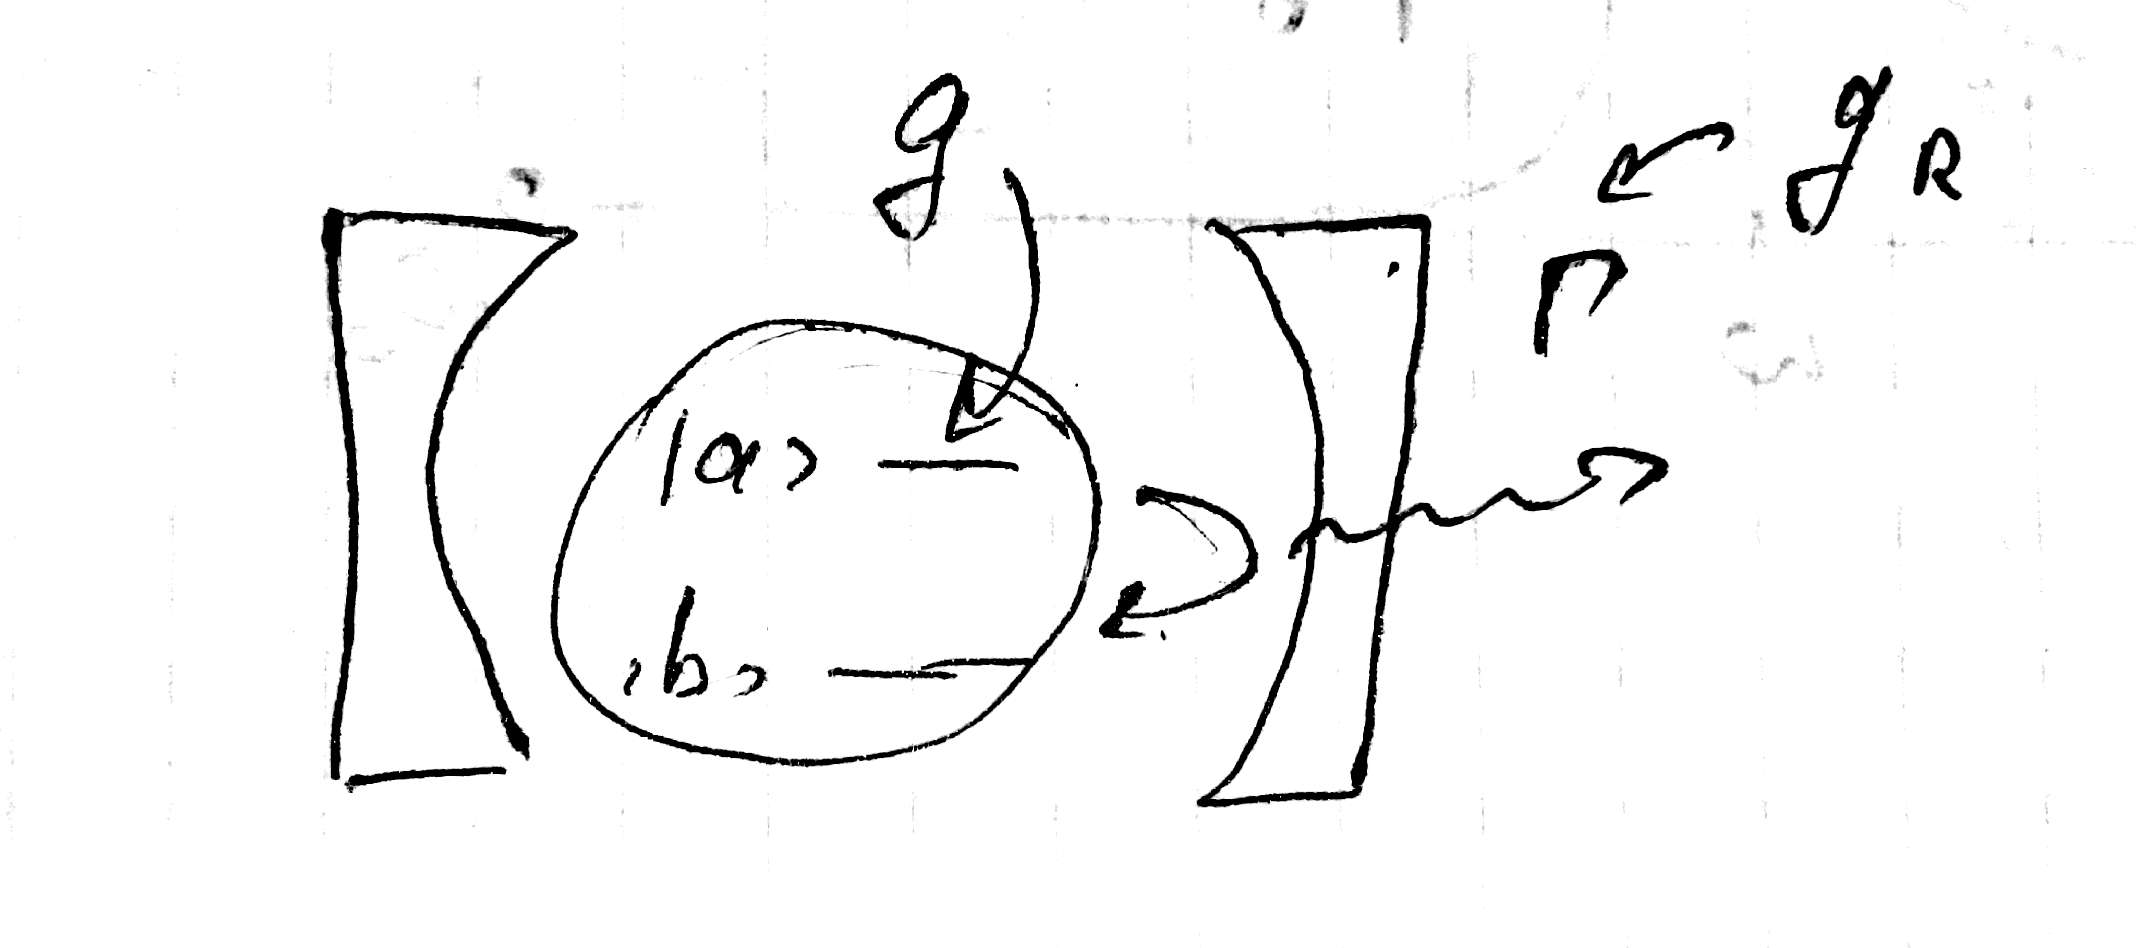
\includegraphics[width=0.3\linewidth]{fig/L10/atom_in_R}
	\caption{Atom in a cavity with losses. System has two coupling constants: $g$ --- atom and field coupling, $\Gamma$ --- cavity and reservoir coupling (transparency of a mirror)}
	\label{fig:atominr}
\end{figure}

\subsection{The Purcell factor for a closed cavity}

The decay rate $\gamma$ can be written as
\begin{equation}
	\gamma = 2 \pi \left| g(\omega) \right|^2 \frac{D(\omega)}{V},
	\label{eq:gamma}
\end{equation}
where $D/V = \rho$ is the density of state. In vacuum it is $D_0(\omega) = \frac{\omega^2}{\pi^2 c^3}$ but in a cavity it can be approximated by the Lorentzian (fig) with resonant frequency $\omega_0$
\begin{equation}
	D(\omega) = \frac{1}{\pi} \frac{\omega_{0}/2Q}{(\omega - \omega_{0})^2 + \left( \omega_{0}/2Q \right)^2}.
\end{equation}

\begin{figure}
	\centering
	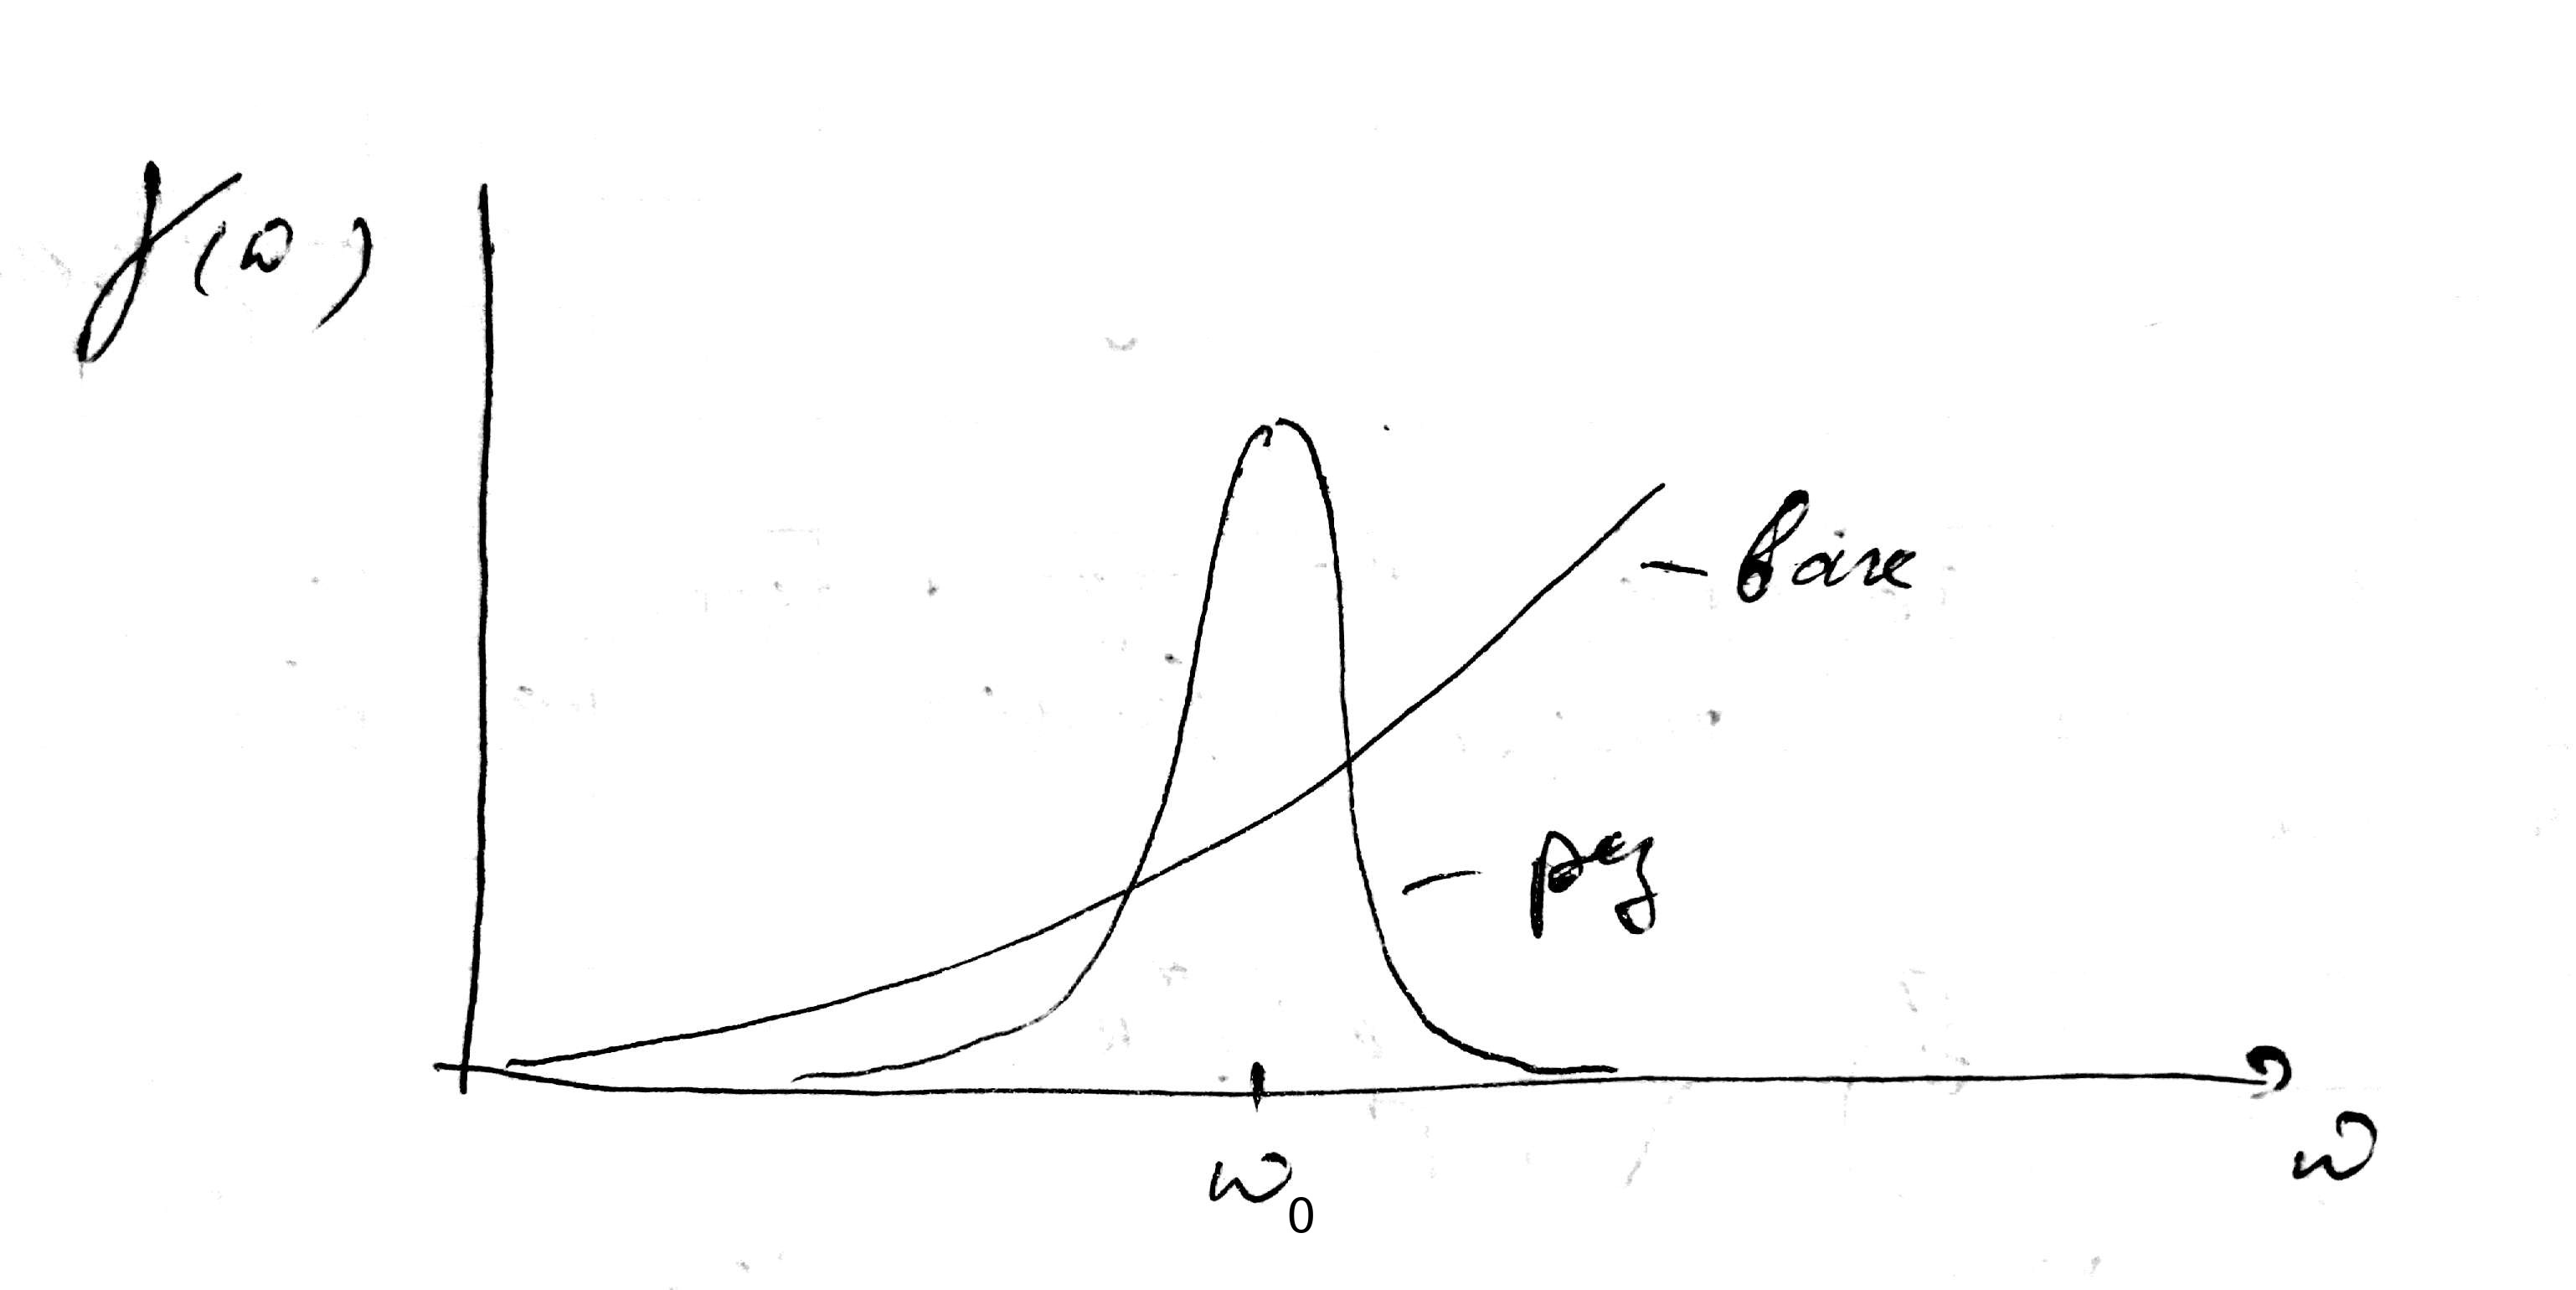
\includegraphics[width=0.5\linewidth]{fig/L10/gamma}
	\caption{The decay rate in vacuum and in a cavity}
	\label{fig:gamma}
\end{figure}

There two cases which is interesting to consider:
\begin{enumerate}
	\item[\textit{Case 1.}] $\omega \approx \omega_0$ --- transition and cavity frequencies are approximately equal. Then
	\begin{equation}
		D(\omega = \omega_0) \approx \frac{1}{\pi} \frac{2Q}{\omega_0}.
	\end{equation}
	Substitution to \eqref{eq:gamma} gives
	\begin{equation}
		\gamma = 2\pi \left| g(\omega) \right|^2 \frac{2Q}{\pi \omega} \frac{1}{V} = \underbrace{2\pi \left| g(\omega) \right|^2 \frac{\omega^2}{\pi^2 c^3}}_{\hookrightarrow=\gamma_0} \cdot \frac{1}{V} \frac{\pi^2 c^3}{\omega^2} \cdot \frac{2Q}{\pi \omega} = \gamma_0 \frac{1}{\left(2\pi\right)^2} \frac{\lambda^3}{V} Q,
	\end{equation}
	so the Purcell factor for a cavity is strongly depends on the $\lambda^3/V$ and the quality factor $Q$:
	\begin{equation}
		\boxed{F_{\text{P}} = \frac{\gamma}{\gamma_0} = \frac{1}{\left(2\pi\right)^2} \cdot \frac{\lambda^3}{V} Q.}
	\end{equation}
	
	\item[\textit{Case 2.}] $\left|\omega_0 - \omega\right| \gg \Gamma = \omega_0 / Q$. In this case we have
	\begin{equation}
		D(\omega) \approx \frac{1}{\pi} \frac{\Gamma}{2 \omega^2} = \frac{1}{2\pi} \frac{1}{Q \omega},
	\end{equation}
	then
	\begin{equation}
		F_{\text{P}} = \frac{\gamma}{\gamma_0} = \frac{1}{\left(2\pi\right)^2} \frac{\lambda^3}{V} \cdot \frac{1}{Q}.
	\end{equation}
	Usually $Q \gg 1$ and $\frac{\lambda^3}{V} \sim 1$, so far from the resonance $F_{\text{P}} \ll 1$.
\end{enumerate}

\subsection{Rigorous derivation of the atomic decay}

If the approach is rigorous then we have to call Mr. Hamiltonian immediately
\begin{equation}
	\hat{\mathcal{H}} = \hat{\mathcal{H}}_{\text{A}} + \hat{\mathcal{H}}_{\text{F}} + \hat{\mathcal{H}}_{\text{AF}} + \hat{\mathcal{H}}_{\text{R}} + \hat{\mathcal{H}}_{\text{RF}},
\end{equation}
where A stands for atom, F for field and R for reservoir. Summands of $\hat{\mathcal{H}}$ are the following
\begin{equation}
	\hat{\mathcal{H}}_{\text{F}} = \hbar \omega \hat{n}, \qquad \hat{\mathcal{H}}_{\text{A}} = \half \hbar \omega_0 \hat{\sigma}_z, \qquad \hat{\mathcal{H}}_{\text{R}} = \sum_{\kv} \hbar \omega_{\kv} \hat{n}_{\kv},
\end{equation}
\begin{equation}
	\hat{\mathcal{H}}_{\text{AF}} = \hbar g \left( \hat{\sigma}_+ \hat{a} + \hat{a}^{\dagger} \hat{\sigma}_- \right),  \qquad \hat{\mathcal{H}}_{\text{FR}} = \hbar \sum_{\kv} g_{\kv} \left( \hat{a}^{\dagger} \hat{b}_{\kv} +  \hat{b}^{\dagger}_{\kv} \hat{a} \right), \qquad 
	g, g_{\kv} \in \mathbb{R}.
\end{equation}

We are interested in time dependence of $\av{\hat{\sigma}_z}$ and $\av{\hat{a}^{\dagger} \hat{a}}$. Angle brackets represents the averaging over the reservoir and quantum mechanics averaging $\av{\dots} \equiv \av{\av{\dots}_{\text{R}}}_{\text{QM}}$. For an any atom operator $\hat{O}_{\text{A}}$ we have a supporting relation
\begin{equation}
	\frac{d}{dt} \av{(\hat{a}^{\dagger})^m (\hat{a})^n \hat{O}_{\text{A}} }= - \frac{i}{\hbar} \left[ (\hat{a}^{\dagger})^m (\hat{a})^n \hat{O}_{\text{A}}, \hat{\mathcal{H}}_{\text{A}} + \hat{\mathcal{H}}_{\text{F}} + \hat{\mathcal{H}}_{\text{AF}} \right] + \frac{d}{dt} \av{ (\hat{a}^{\dagger})^m (\hat{a})^n } \hat{O}_{\text{A}}.
\end{equation} 
Similar to \eqref{eq:dn} it is not so hard to obtain the answer for a any positive integer powers 
\begin{multline}
	\frac{d}{dt} \av{(\hat{a}^{\dagger})^m (\hat{a})^n} = \left[ i \omega (m-n) - \frac{\Gamma}{2}(m+n) \right] \av{(\hat{a}^{\dagger})^m (\hat{a})^n} + \\ + \Gamma\cdot  mn \cdot \bar{\hat{n}}_{\text{R}} \av{(\hat{a}^{\dagger})^{m-1} (\hat{a})^{n-1}}.
\end{multline}
In the particular case, when $\hat{O}_{\text{A}} = \hat{\mathbb{1}}$, we have
\begin{equation}
	\frac{d}{dt} \av{\hat{a}^{\dagger} \hat{a}} = - \frac{i}{\hbar} \av{\left[ \hat{a}^{\dagger} \hat{a}, \hat{\mathcal{H}}_{\text{A}} + \hat{\mathcal{H}}_{\text{F}} + \hat{\mathcal{H}}_{\text{AF}} \right]} - \Gamma \av{\hat{a}^{\dagger} \hat{a}} + \Gamma \bar{\hat{n}}_{\text{R}}.
\end{equation}
As the commutator of $\hat{a}$ is trivial $\left[\hat{a}, \hat{a}^{\dagger}\right]=1$, so
\begin{equation}
	\left[ \hat{a}^{\dagger} \hat{a}, g \left( \hat{\sigma}_+ \hat{a} + \hat{a}\dag \hat{\sigma}_-\right) \right] =  g \hat{a}\dag \hat{\sigma}_- - g \hat{\sigma}_+ \hat{a},
\end{equation}
then
\begin{equation}
	\frac{d}{dt} \av{\hat{a}^{\dagger} \hat{a}} = - \frac{i}{\hbar} g\underbrace{\av{\hat{a}\dag \hat{\sigma}_- - \hat{\sigma}_+ \hat{a}}}_{?} - \Gamma \av{\hat{a}^{\dagger} \hat{a}} + \Gamma \bar{\hat{n}}_{\text{R}},
	\label{eq:aa}
\end{equation}
where $\av{\hat{a}\dag \hat{\sigma}_- - \hat{\sigma}_+ \hat{a}}$ is yet unknown.

Now let us take a look at sigma--$z$ operator
\begin{equation}
	\frac{d}{dt} \av{\hat{\sigma}_z} = -\frac{i}{\hbar} \av{\left[ \hat{\sigma}_z, g \hat{a}\dag \hat{\sigma}_- + g \hat{\sigma}_+ \hat{a} \right]} = 2 g\frac{i}{\hbar} \underbrace{\av{\hat{a}\dag \hat{\sigma}_- - \hat{\sigma}_+ \hat{a}}}_{?},
	\label{eq:sigmaz}
\end{equation}
where we have got the same unknown averaging. To obtain last result the commutation relations for $\sigma$--matrices had been used:
\begin{equation}
	\left[ \hat{\sigma}_z, \hat{\sigma}_- \right] = - 2 \hat{\sigma}_-, \qquad
	\left[ \hat{\sigma}_z, \hat{\sigma}_+ \right] = 2 \hat{\sigma}_+.
\end{equation}

To solve \eqref{eq:aa} and \eqref{eq:sigmaz} we need to know the time dependence of that unknown Hermitean operator $\av{\hat{a}\dag \hat{\sigma}_- - \hat{\sigma}_+ \hat{a}}$, which equation of motion involves the quantity $\av{\hat{a}\dag \hat{\sigma}_z \hat{a}}$ and so on. In general, we get an infinite set of equations which may not be analytically solvable. The way out is the following --- we need to cut the chain of equations at some step. Here the things we are going to suppose:
\begin{enumerate}
	\item Put cavity at zero temperature reservoir ($\bar{\hat{n}}_{\text{R}} = 0$).
	\item Initially the atom is in the excited sate $\ket{a}$ and field inside the cavity is in the vacuum state $\ket{0}$.
\end{enumerate}
In other words, we consider \textit{a single photon approximation}. If the photon is only one then all summands which are proportional to $\hat{a}^2$ or $\hat{a}^{\dagger 2}$ are identically zero. As the result, under these conditions, we obtain the following system of equations:
\begin{equation}
	\begin{cases}
		\frac{d}{dt} \av{\hat{a}\dag \hat{a}} = g \chi(t) - \Gamma \av{\hat{a}\dag\hat{a}} \\
		\frac{d}{dt} \av{\hat{\sigma}_z} = - 2 g \chi(t) \\
		\frac{d}{dt} \chi(t) = g \av{\hat{\sigma}_z} + 2 g \cdot y(t) + g - \frac{\Gamma}{2} \chi(t) \\
		\frac{d}{dt} y(t) = - g \chi(t) - \Gamma y(t)
	\end{cases},
	\qquad 
	\begin{matrix}
		\chi(t) &\myeq& i \av{\hat{\sigma}_+ \hat{a} - \hat{a}\dag\hat{\sigma}_-}, \\
		y(t) &\myeq& \av{\hat{a}\dagger\hat{\sigma}_z \hat{a}}, \qquad \quad \ 
	\end{matrix}
\end{equation}
with the initial conditions 
\begin{equation}
	\chi \big|_{t=0} = 0, \qquad y \big|_{t=0} = 0, \qquad \av{\hat{a}\dag\hat{a}} \big|_{t=0} = 0, \qquad \av{\hat{\sigma}_z} \big|_{t=0} = 1. 
\end{equation}

Using the single photon approximation is always simplifies the problem and make it look more "classical".

This system has two main parameters: $g$ and $\Gamma$ (see fig. \ref{fig:atominr}). Let us consider two limiting behavior regimes:
\begin{enumerate}
	\item[\textit{Regime 1.}] $\Gamma \gg g \to \Gamma \gg \Omega_R$ or a  \textit{overdamping} regime. Here we have
	\begin{equation}
		\av{\hat{\sigma}_z} = -1 + 2 e^{-4 g^2 \frac{t}{\Gamma}} = - 1 + 2e^{- \gamma t},
	\end{equation}
	where 
	\begin{equation}
		\gamma = \frac{4 g^2}{\Gamma} = \frac{4 g^2 Q}{\omega} = \underbrace{\frac{6\pi c^3 Q}{V \omega^2}}_{F_{\text{P}}} \cdot \frac{8 \left|\vec{d}\right|^2 \omega^2}{\hbar \omega_0 c^3} \quad \to \quad \gamma \sim F_{\text{P}}.
	\end{equation}
	The cavity increase the dissipation rate!
	\item[\textit{Regime 2.}] $\Gamma \ll g$ or a \textit{low losses} regime. Here we can obtain that the atomic inversion $\av{\hat{\sigma}_z}$ is
	\begin{equation}
		\av{\hat{\sigma}_z} = - 1 + e^{- \frac{\Gamma}{2} t} \left[1 + \cos \left( 2 gt \right)\right]
	\end{equation}
	so the probability $P_a$ take the simple form
	\begin{equation}
		P_a = \av{\hat{\sigma}_z} + 1 = e^{- \frac{\Gamma}{2} t} \left[1 + \cos \left( 2 gt \right)\right]
	\end{equation}
\end{enumerate}
Different regimes are represented on a fig. \ref{fig:regimes}.

\begin{figure}
	\centering
	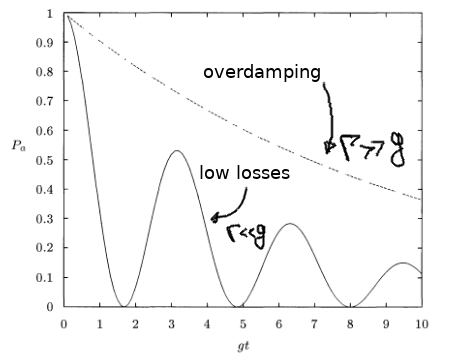
\includegraphics[width=0.7\linewidth]{fig/L10/regimes}
	\caption{Probability $P_a$ versus dimensionless time $gt$ for the different limiting behavior regimes.}
	\label{fig:regimes}
\end{figure}

	
\end{document} 